\section{Electro-optical setup}\label{electro-optical-setup}

\subsection{Run 7 Optical modifications}\label{run-7-optical-modifications}

For Run 7 there were a few changes with our setup on Level 3 as compared
to Run 6 taken in IR2 at SLAC. One of the changes was that we did not
have access to the CCOB Narrow/Thin beam. .. While the set up was on
Level 3, we did not have the resources or expertise to get it setup. As
such, the majority of the testing was done with the CCOB Wide Beam
projector. We did obtain an additional projector, the 4k projector, part
way through Run 7 that will be discussed later. With the CCOB Wide Beam,
we used a cone attached to the L1 cover as well as shroud to create a
dark environment as seen below.

\begin{table}[htbp]
\centering
\begin{tabular}{cc}
    % 左側の画像(幅を調整)
    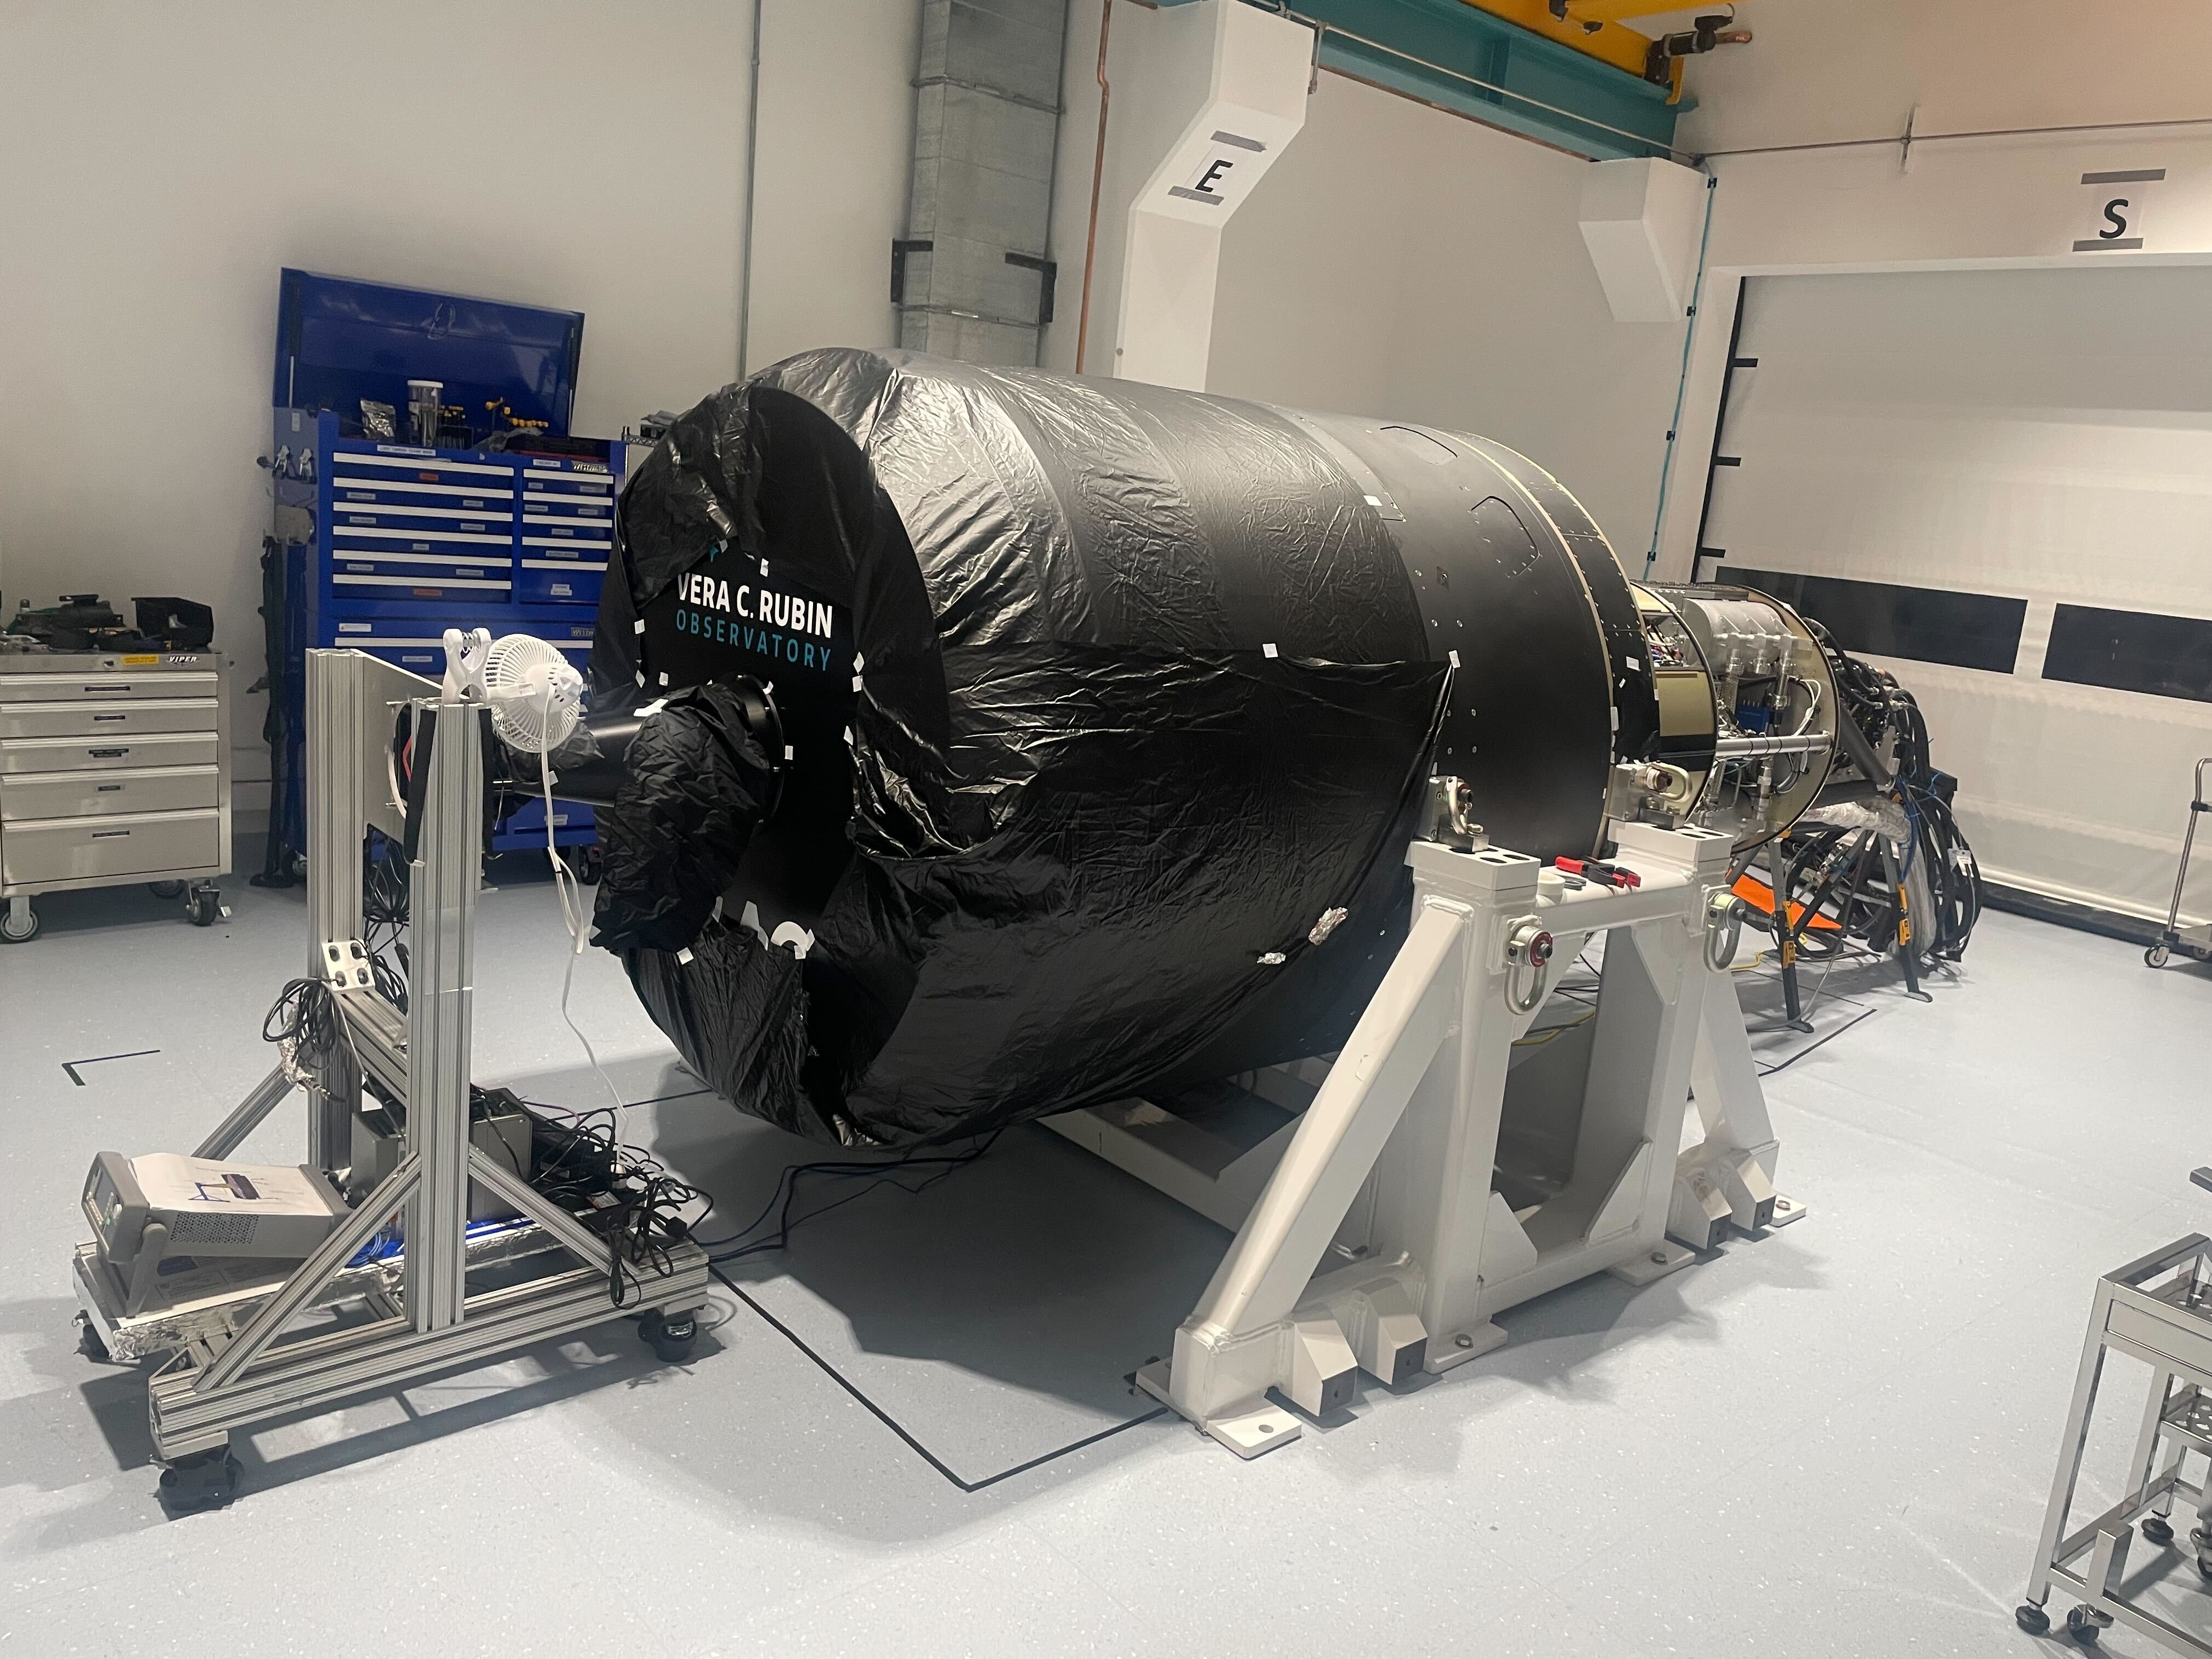
\includegraphics[width=0.45\textwidth]{sections/figures/Camera_Shroud.jpg} &
    % 右側の画像(幅を調整)
    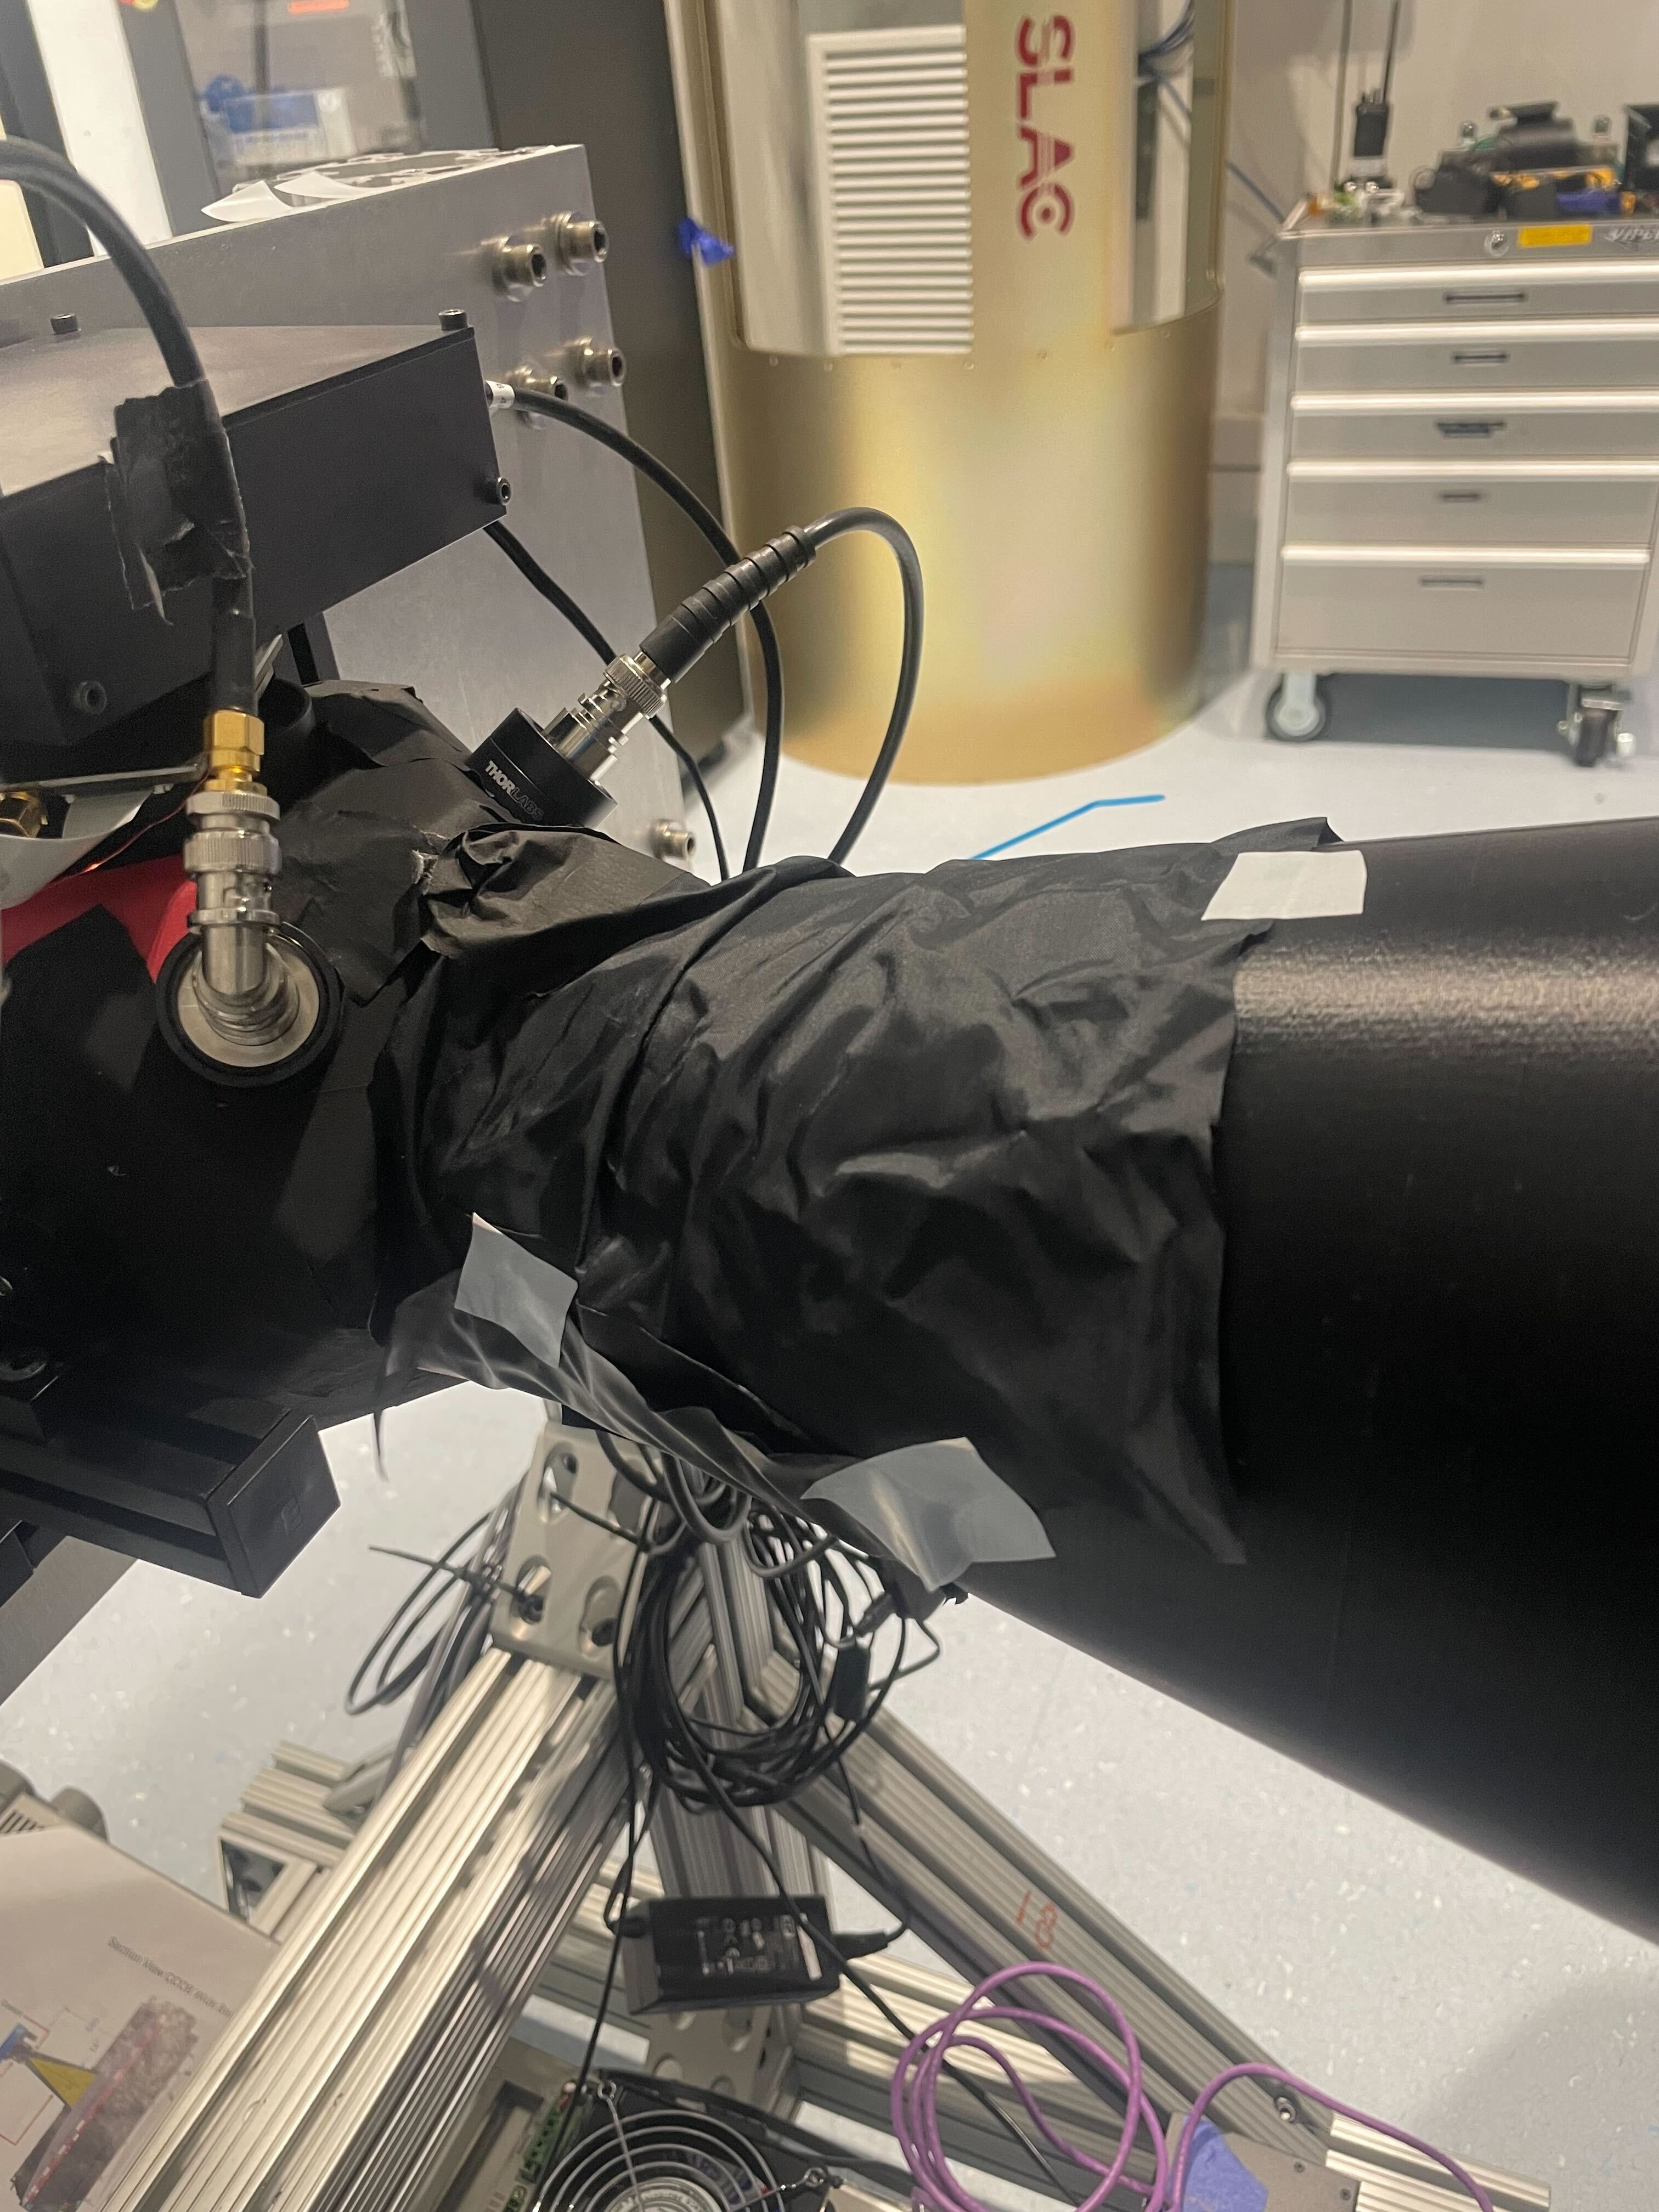
\includegraphics[width=0.45\textwidth]{sections/figures/CCOB_Wide_Shroud.jpg} \\
\end{tabular}

\caption{Final shroud configuration of LSSTCam in Level 3 to reduce light leaks.}
\caption*{CCOB Wide Beam attached to the cone and shrouded.}
\end{table}

This allowed us to operate on Level 3 with a dark current of
\textless0.1 ADU/sec with the shutter open. The initial set up of the
CCOB Wide Beam was the same as Run 6, we had a minimal ND filter (10 \%)
attached to a C-mount lens. One change was that the f/stop of the lens
was changed from 2.6 to 1.6 (fully open). This was done to try and
reduce the effect of the \textquotesingle weather\textquotesingle{} and
the \textquotesingle CMB patten\textquotesingle{} two effects that we
found in Run 6 and were found to be due to our projection setup (see
\hyperref[Banovetz2024]{{[}Banovetz2024{]}}), While changing it did
reduce the weather pattern, it also caused a much steeper roll off
across the focal plane. The below figures show the weather pattern as
compared to Run 6 and the rolloff of the light as compared to Run 6.

\begin{figure}[htbp]
\centering
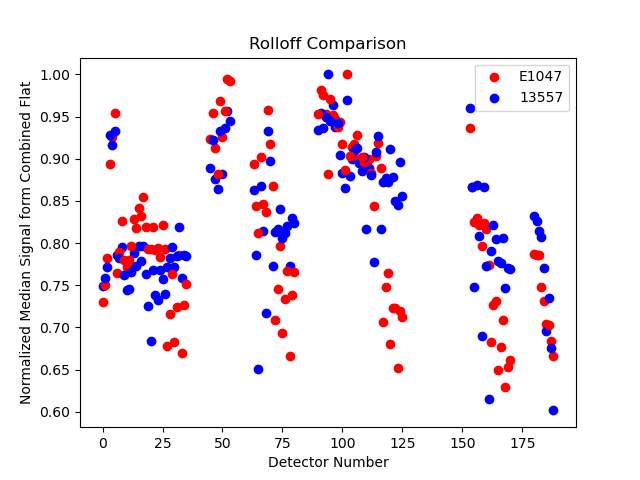
\includegraphics[width=0.9\textwidth]{sections/figures/Run7_DiffuserIllumination.png}
\caption{Illumination across the focal plane from Run 7 with the diffuser as compared to Run 6.}
\end{figure}

To both reduce the effect of the
\textquotesingle weather\textquotesingle{} and
\textquotesingle CMB\textquotesingle{} but retain uniform illumination
across the focal plane, we installed a diffuser in the cone attached to
L1. Below shows the placement of the diffuser along the cone.

\begin{figure}
\centering
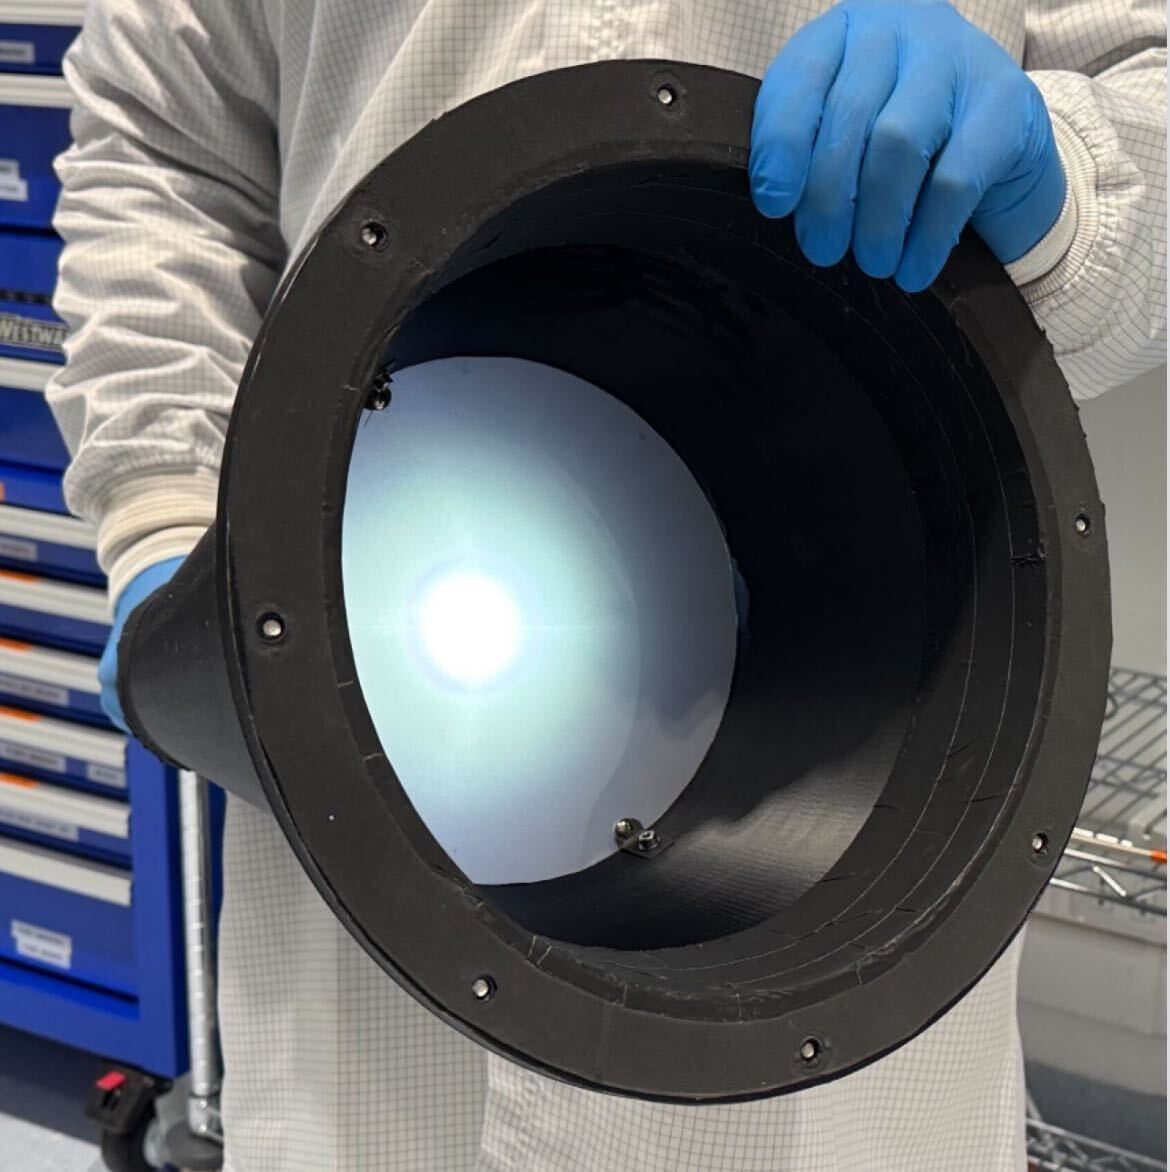
\includegraphics[width=0.9\textwidth]{sections/figures/Diffuser.jpg}
\caption{Diffuser installed into the light cone.}
\end{figure}

The diffuser combined with a fully open F/stop effectively reduced the
incoming light by roughly 35\%. Adjusting for that, we found that it
severly reduced the \textquotesingle weather\textquotesingle{} and
eliminated the CMB pattern, as well as fully illuminateing the focal
plane. Below shows the effect of the diffuser in regards to the weather,
CMB, and the overall illumination of the focal plane.

\begin{figure}[htbp]
\centering
\begin{minipage}{0.45\textwidth}
    \centering
    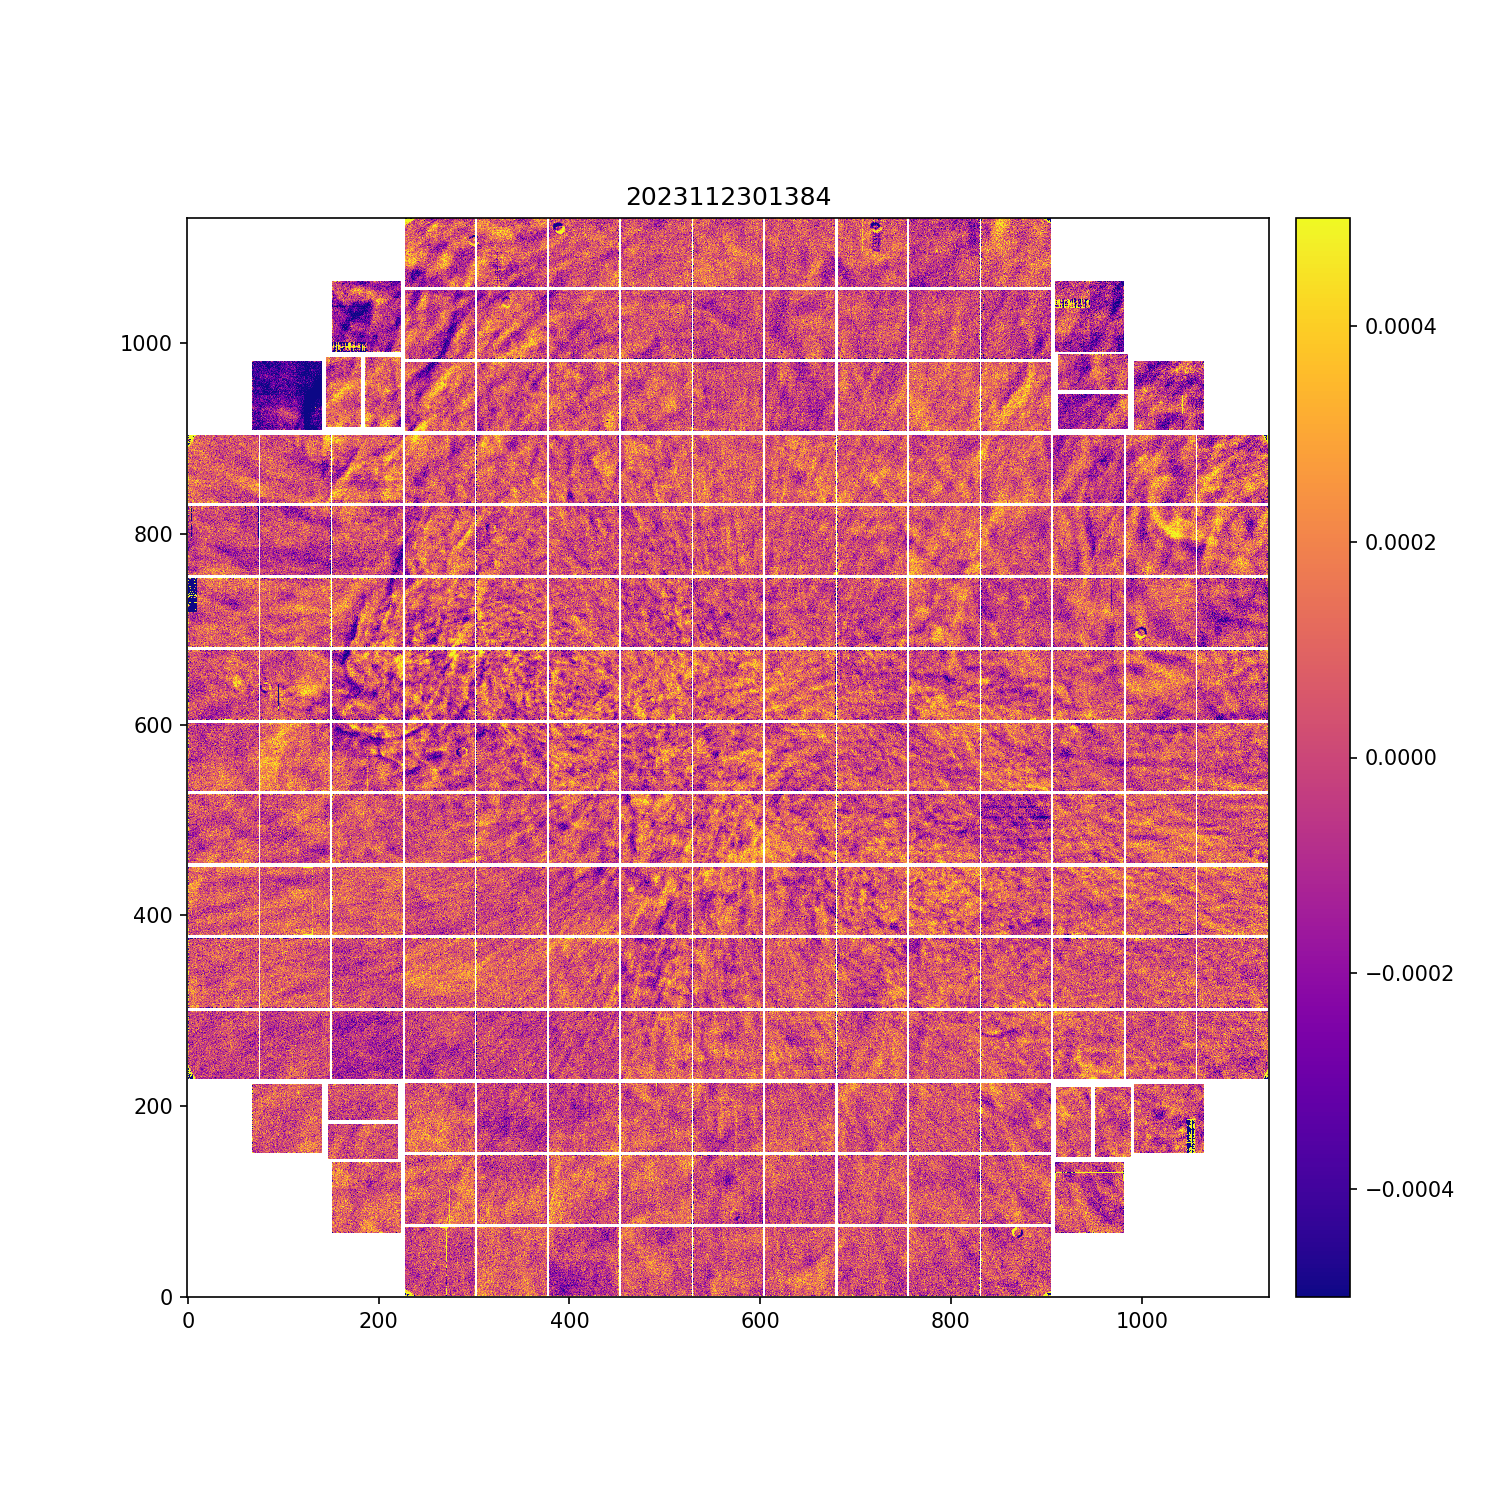
\includegraphics[width=\linewidth]{sections/figures/Run6_Weather.png}
    \caption{Full focal plane image showing the fractional difference in Run 6.}
\end{minipage}
\hfill
\begin{minipage}{0.45\textwidth}
    \centering
    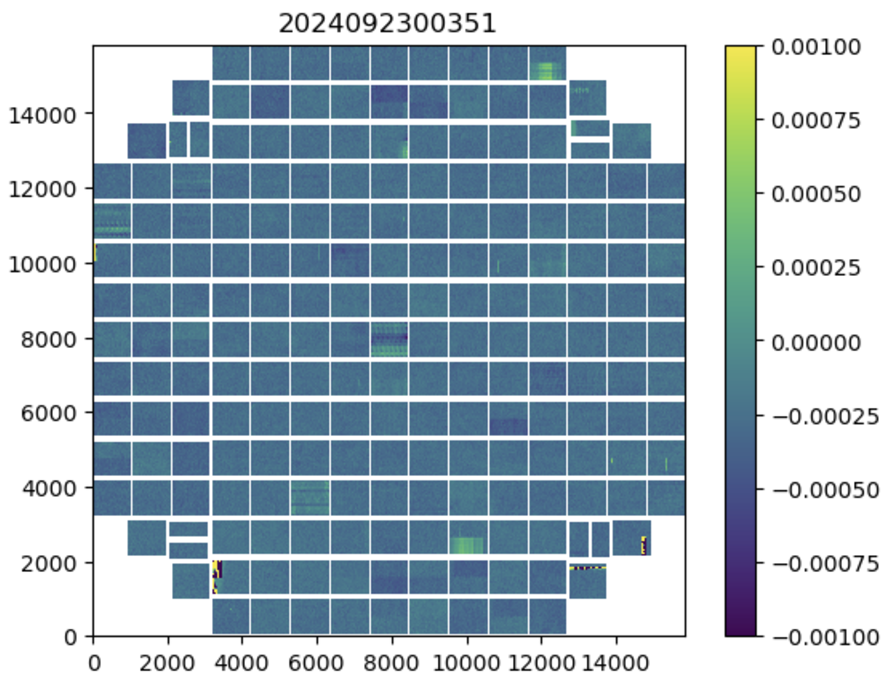
\includegraphics[width=\linewidth]{sections/figures/Run7_WeatherDiffuser.png}
    \caption{Full focal plane image showing the fractional difference in Run 7.}
\end{minipage}
\end{figure}

\begin{figure}
\centering
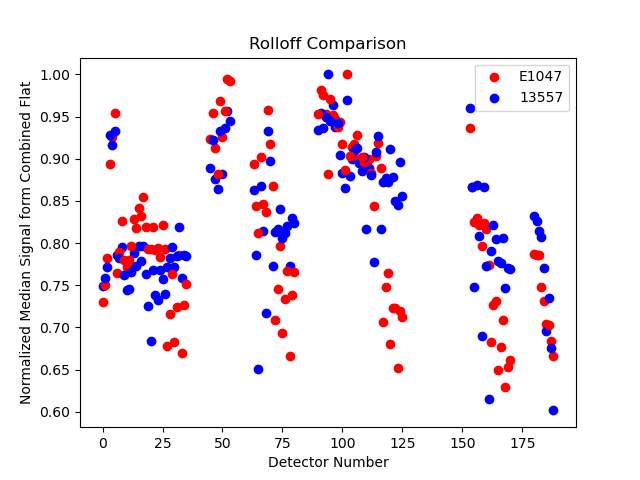
\includegraphics[width=0.9\textwidth]{sections/figures/Run7_DiffuserIllumination.png}
\caption{Illumination across the focal plane from Run 7 with the
diffuser () as compared to Run 6 ().}
\end{figure}

The diffuser was installed for all B protocol and PTC runs moving
forward, only being taken out for pinhole projection and when using the
4K projector.

The newest addition to the projectors used for EO testing was a 4K
projector, simliar to those used in conference rooms. This projector was
first tested at SLAC before coming to Chile around half through Run 7.
This was used primarily as a spot projector, as the pinhole filter
wasn\textquotesingle t operational but more importantly, this could
illuminate all 3206 amplifiers instead of the 21 illuminated by the
pinhole projector. Most runs included the spots and the spot fluxes were
controlled by the shutter instead of any flashing (e.g. CCOB Wide). One
downside that was found was that the illumination of
\textquotesingle dark\textquotesingle{} regions (regions not supposed to
be illuminated) were still giving off light. This background region had
structure that changed with time and could not be easily subtracted. It
also caused the contrast between the spot and the background to be
around 6. Changing the shape to large rectangles for crosstalk
measurements increased this contrast to 30.

\subsection{Projector spots}\label{projector-spots}

hello world.

This section describes the spots and rectangles tested with the 4k
projector

\begin{itemize}
\tightlist
\item
  Projector background
\item
  Spots on many amps
\item
  Spots on one amp
\item
  Optical setup
\end{itemize}

\subsection{Dark current and light
leaks}\label{dark-current-and-light-leaks}

This section describes dark current and light leaks in Run 7 testing.

\subsubsection{Light leak mitigation with shrouding the camera
body}\label{light-leak-mitigation-with-shrouding-the-camera-body}

One of the first tests we attempted with the camera was measuring dark
current and sources of light leaks in the camera body. This began by
finding gaps between the L1 cover and the gaskets. This was covered up
by tape where we felt comfortable applying it. Below shows the gaps that
we could see between L1 and its cover.

\begin{figure}
\centering
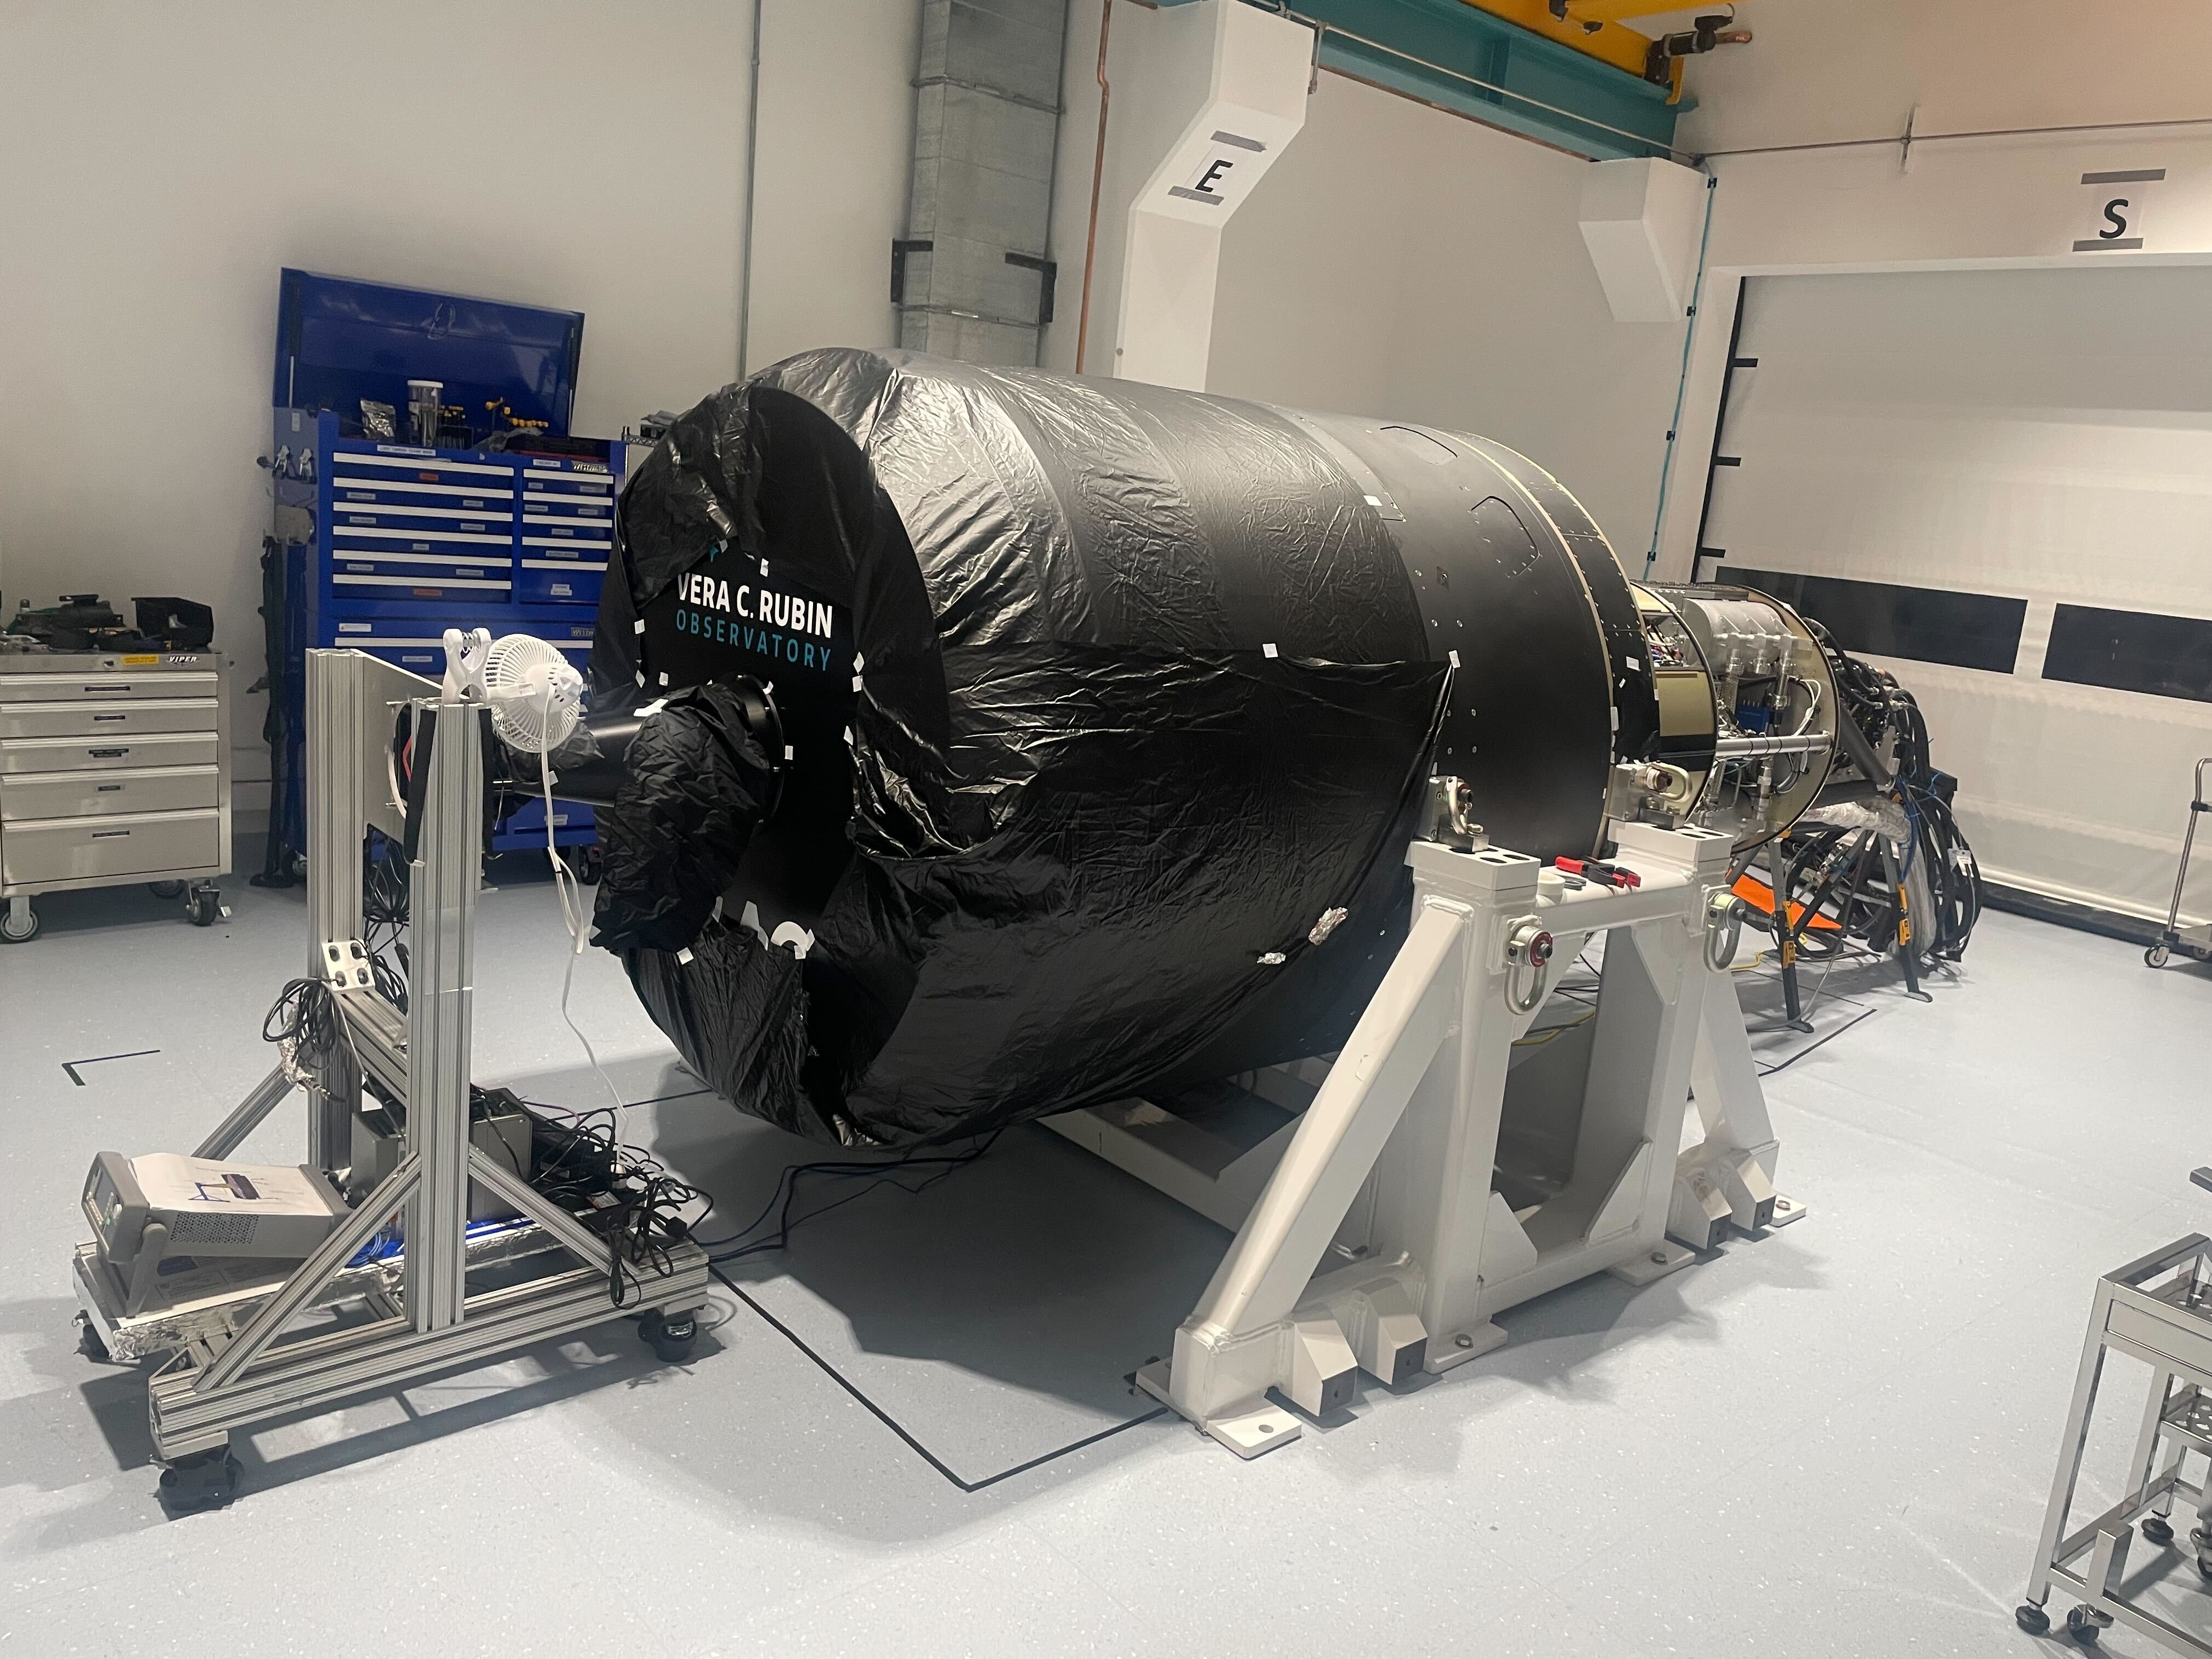
\includegraphics[width=0.9\textwidth]{sections/figures/Camera_Shroud.jpg}
\caption{}
\end{figure}

Once these were sealed, we took some intital measurements and then
started to cover the camera body with shroud. We also found light leaks
where the light cone attached to L1 was housed, and from the utility
trunk. Below is the table of observations, their corressponding dark
current, and comments on what changed.

\phantomsection\label{light_leak}

\begin{longtable}{|l|l|l|l|l|}
\caption{Table showing the different 15 second dark exposures, the different conditions, and the resulting dark current.
Exposure ID is preceded by "MC\_C202409".  ("Initial Covering" was just the CCOB cone and around the L1 cover)} \\
\hline
\textbf{Exposure} & \textbf{Dark Current} & \textbf{Room Lights} & \textbf{Shutter} & \textbf{Comments} \\
\hline
\endfirsthead
\hline
\textbf{Exposure} & \textbf{Dark Current} & \textbf{Room Lights} & \textbf{Shutter} & \textbf{Comments} \\
\hline
\endhead
\hline
\endfoot
\hline
09\_000012 & 0.158 & Off & Closed & \\
09\_000018 & 0.158 & On & Closed & \\
09\_000038 & 2.94 & On & Open & Initial Covering  \\
09\_000054 & 1.34 & On & Open &  + Blanket over the FCS \\
09\_000072 & 0.41 & On & Open &  + Blanket over AND under the FCS \\
09\_000078 & 0.18 & Off & Open & + Blanket over AND under the FCS \\
10\_000031 & 0.033 & On & Open &  + Blanket over AND under the FCS + UT \\
\end{longtable}


Below is a the image of the final shroud configuration covering the
camera.

\begin{figure}
\centering
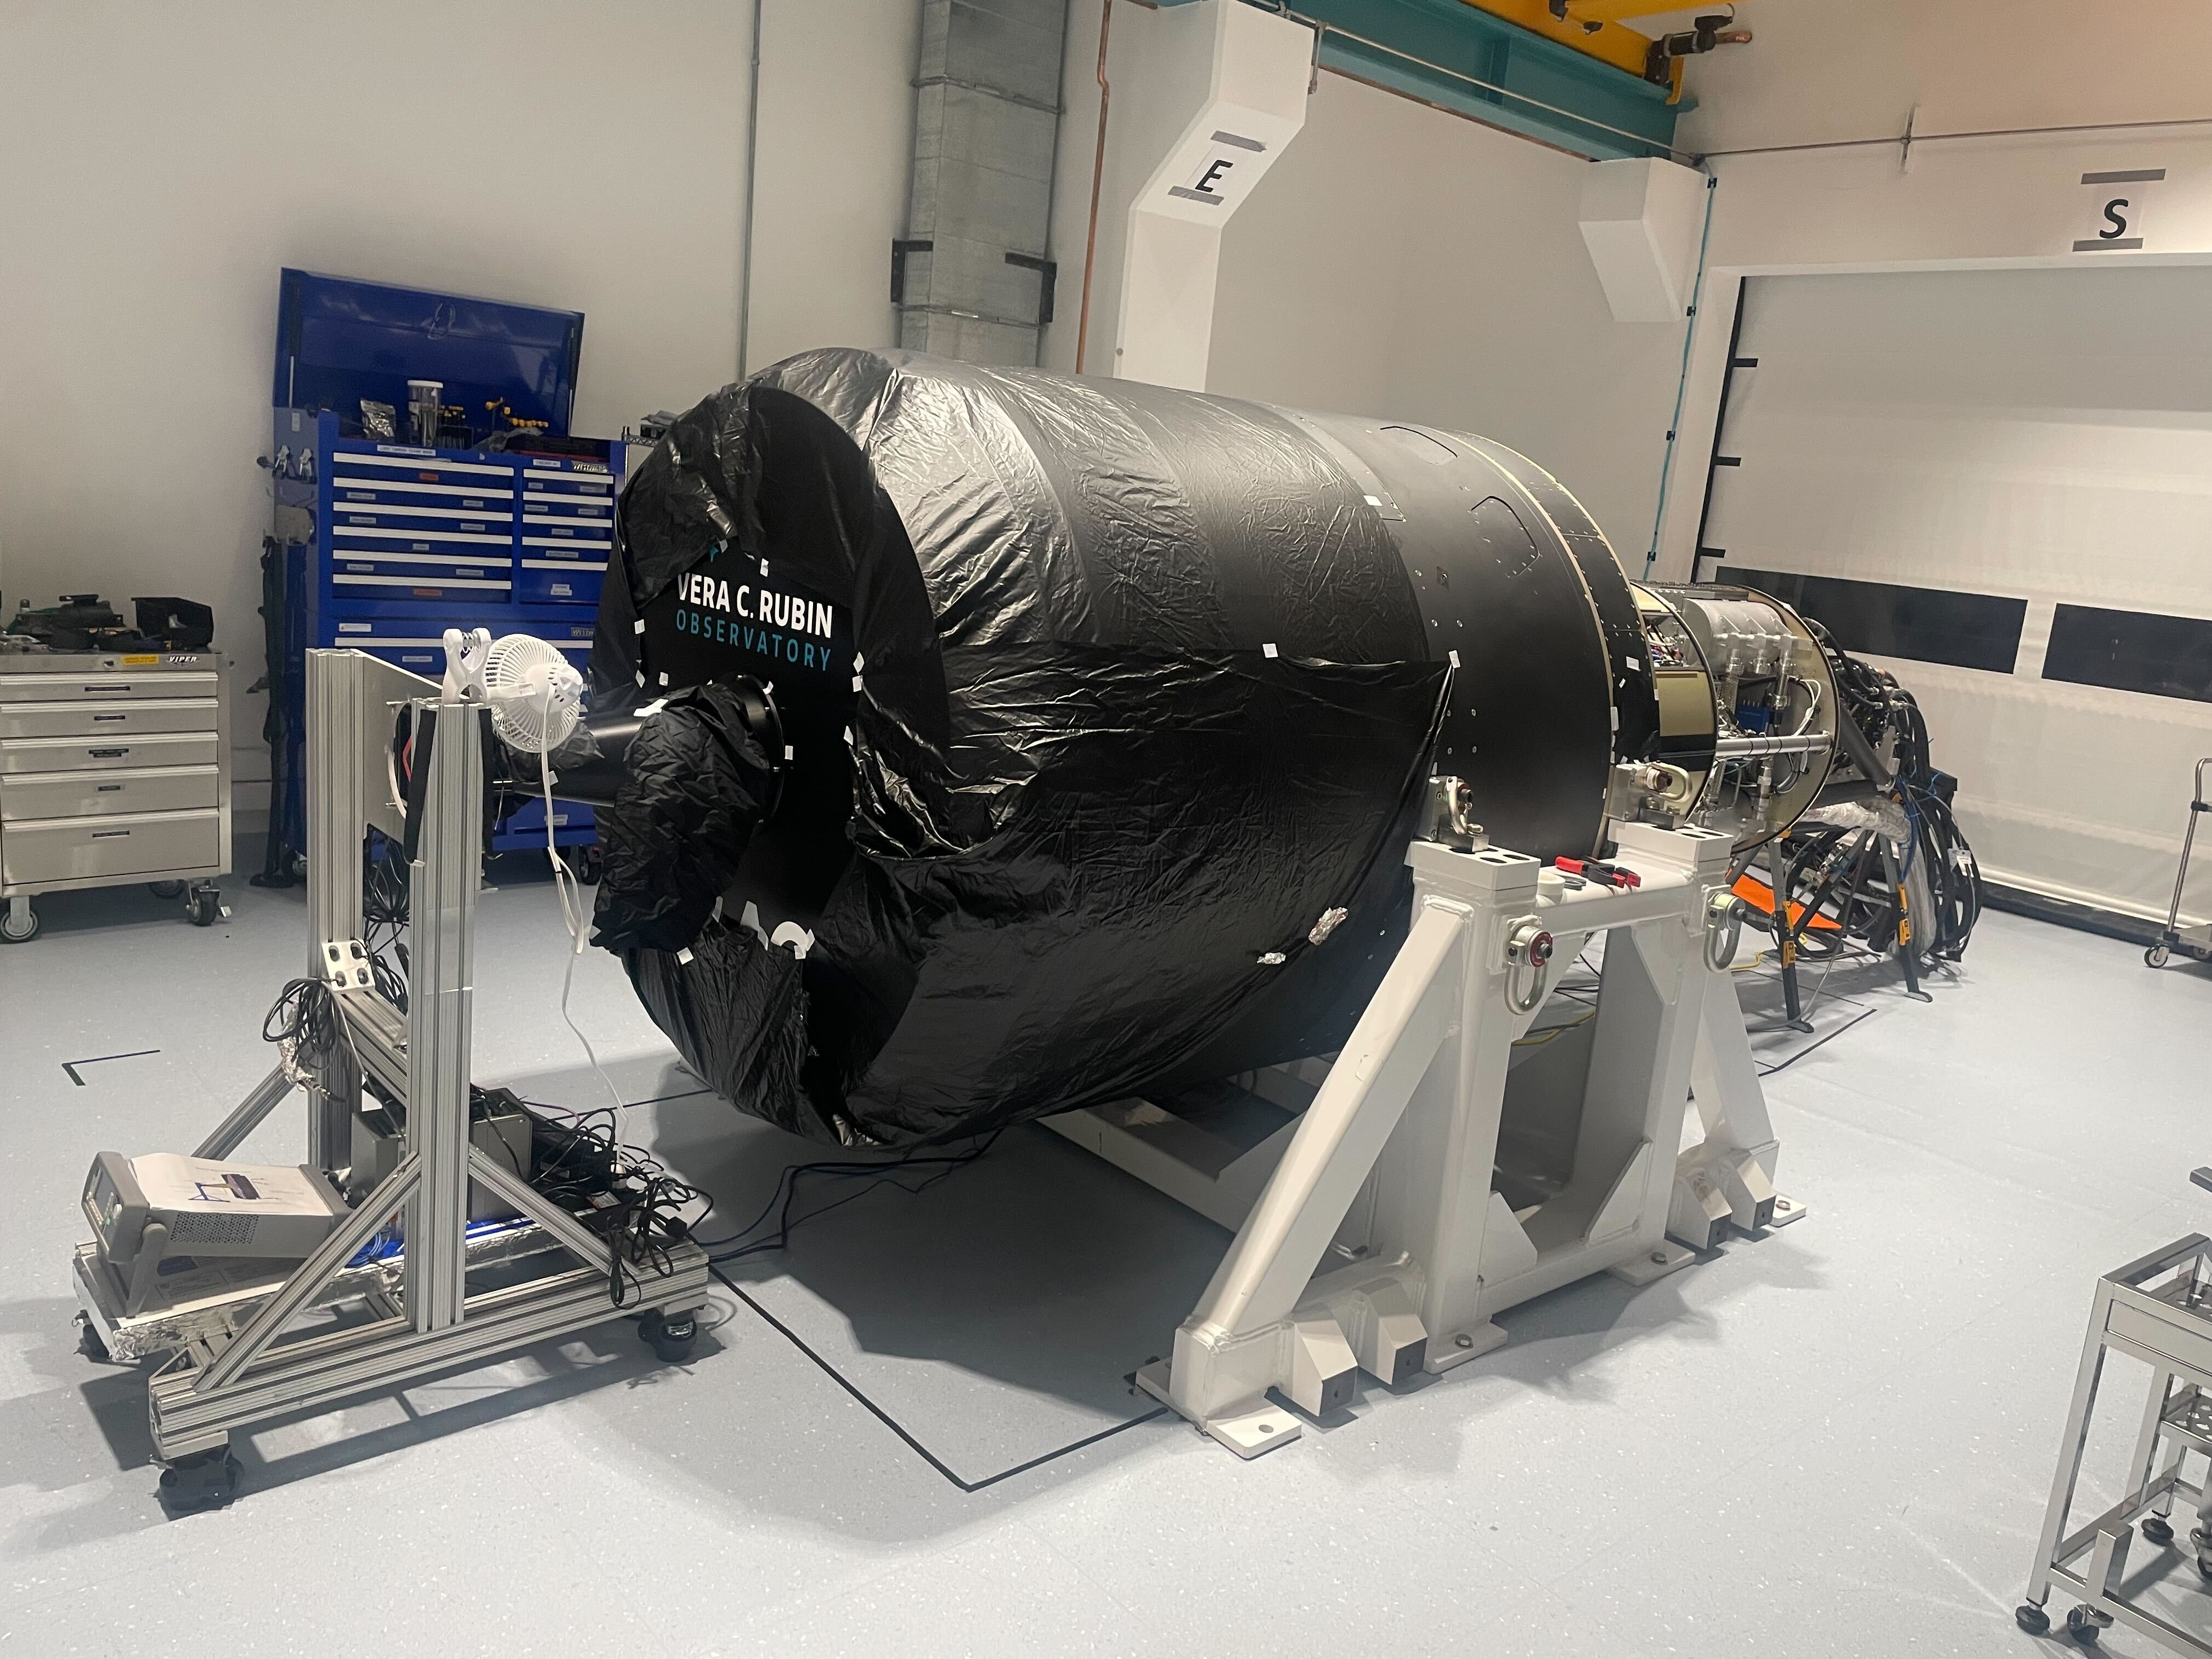
\includegraphics[width=0.9\textwidth]{sections/figures/Camera_Shroud.jpg}
\caption{Final shroud configuration of LSSTCam in Level 3 to reduce
light leaks.}
\end{figure}


\subsubsection{Successful Autochanger Light Leaks
masking}\label{successful-autochanger-light-leaks-masking}

A dedicated dark/light leak study was performed during the Run 6 at SLAC
in summer 2023 and a localized faint light source going up to
\textasciitilde{} 0.04 e-/s/pixel was associated to the 24 V Clean of
the FES auto-changer.

In the Auto-Changer this voltage is used to power some probes and all
controllers. In february 2024, as AC-1 was extracted from the camera for
a global maintenance, a direct investigation to localized the light
source was performed without success. A light source in the AC
wasn\textquotesingle t expected as in the AC all controllers LED have
been removed, and most electronics are in "black boxes". Still two small
probes , which had LEDs that could not be removed, were initially masked
by a black epoxy. As we had doubt on the quality of this masking in the
IR, we applied and extra-making (aluminium black tape) on them during
the Feb 2024 maintenance (on AC 1 and 2).

At the start of the Run 7 a new study of the light leak based on 900s
dark exposures with the shutter open and the empty frame filter en
place, showed that the AC light leaks was still present (
\texttt{see\ left\ plots\ of\ AC\ light\ leak\ \textless{}fig-ac-light-leak\textgreater{}}
). Following this finding, a full review of all the AC hardware powered
by the 24 V dirty was performed, and a candidate was found : the coders
of the 5 main motors of the AC had a partial documentation from the
vendor not mentioning the presence of LED. After interaction with the
vendor the presence of \textasciitilde700nm LEDs incide the coders were
reported. The hypothesis of \textasciitilde700nm LED source has been
found compatible with the observation as no AC light leaks were detected
using the different filters in camera at the start of Run 7 (g,r and y
filters) . A dedicated test in Paris using an AC spare coder and a
precision photometric set-up allowed to identify leak in the masking of
those LED in the vendor packaging. A complementary masking method based
on a 3D printed part + tape + cable tie was qualified in Paris: it is
masking the light leak and it is safe (all parts correctly secured ).

In November 2024, we masked all the lights in the back of level 3 clean
room ( not the part with the camera) to setup a high quality dark room
allowing a direct observation with a CMOS camera of the light leak on
the AC2 motors coders. Also the level of darkness reached, allowed us to
validate the quality of the AC coders light masking. Notice that the
FES-prototype in Paris doesn\textquotesingle t have coder on the Online
Clamps, so we had to tune/qualify directly on the AC2 at summit the
masking of those coders.

For each AutoChanger (1 \& 2), the 5 motors coders with vendor issue on
their LED masking, have been successfully enveloped in a light tight
mask.

Notice that the AC was off starting the Sep 27th at 21:15 UTC in the
first part of the Run 7. For the end of Run 7 (run taken after
mid-November) the AC was back On: as the AC 1 was back in camera with
the new coders light mask in place, we were able to take a new series of
900s dark with AC On \& off, confirming that we had no light leak left
associated to the Filter Exchange System.
(\texttt{see\ right\ plots\ of\ AC\ light\ leak\ \figref{fig-ac-light-leak}})

\begin{figure}
\begin{centering}
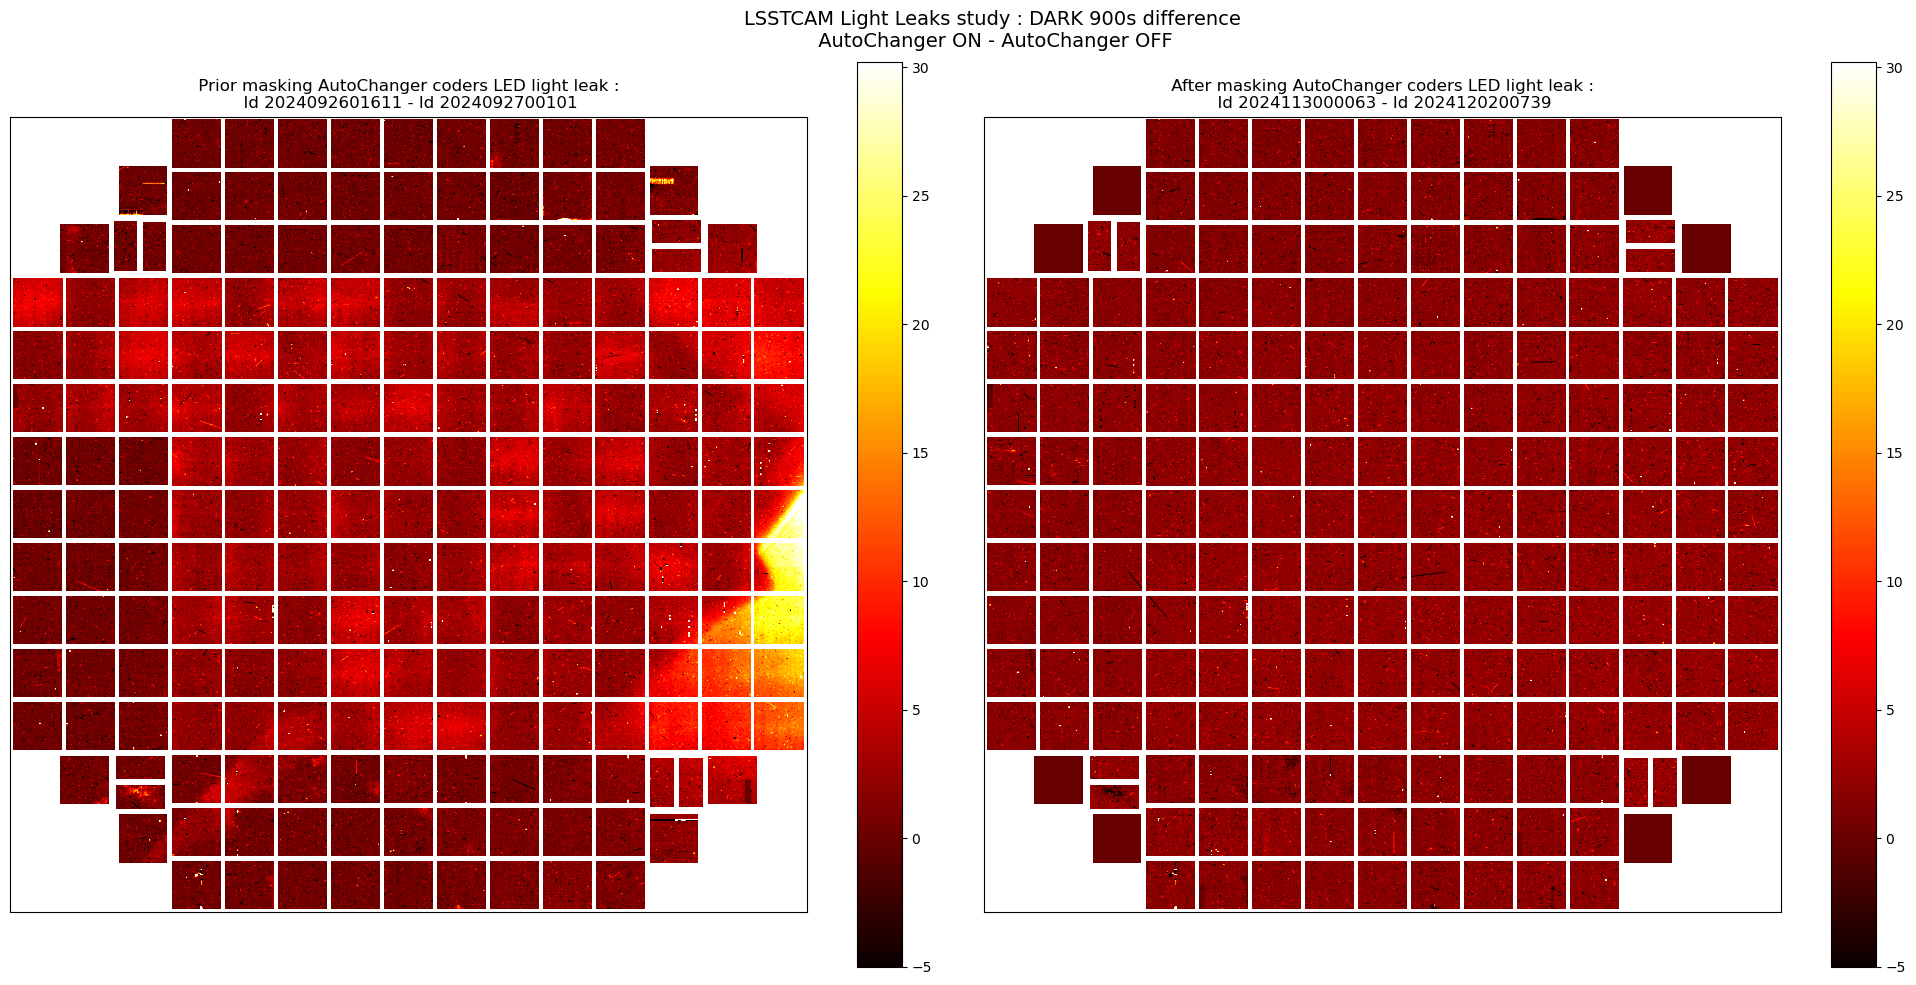
\includegraphics[width=0.8\textwidth]{sections/figures/AC_LightLeak_study.png}
\caption{ The left plot shows the original impact of the AC light leak on 900s dark ( AC On - AC off). On the right plot, after masking the AC LED coders, no light associated to the FES is present in 900s dark difference( FES On - FES off).  \label{fig-ac-light-leak}}
\end{centering}
\end{figure}

\paragraph{Shutter condition impact on
darks}\label{shutter-condition-impact-on-darks}

\paragraph{Filter condition impact on
darks}\label{filter-condition-impact-on-darks}

\subsubsection{Final measurements of dark
current}\label{final-measurements-of-dark-current}

\section{Reverification}\label{reverification}

\subsection{Baseline characterization}\label{baseline-characterization}

\subsubsection{Background}\label{background}

Initial characterization studies performed on LSSTCam were used two
primary acquisition sequences.

\begin{itemize}
\tightlist
\item
  B protocols: this acquisition sequence consists of the minimal set of
  camera acquisitions, including

  \begin{itemize}
  \tightlist
  \item
    Bias images
  \item
    Dark images
  \item
    Flat pairs - flats taken at varying flux levels
  \item
    Stability flats - flats taken at consistent flux levels
  \item
    Wavelength flats - flats taken in different LEDs
  \item
    A persistence dataset - a saturated flat, followed by several darks
  \end{itemize}
\item
  PTCs (photon transfer curves): this acquisition sequence consists of a
  sequence of flat pairs taken at different flux levels. The flat
  acquisition sequence samples different flux levels at a higher density
  than the B protocol flat sequence, enabling a more precise estimate of
  flat pair metrics.
\end{itemize}

\begin{figure}
\begin{centering}
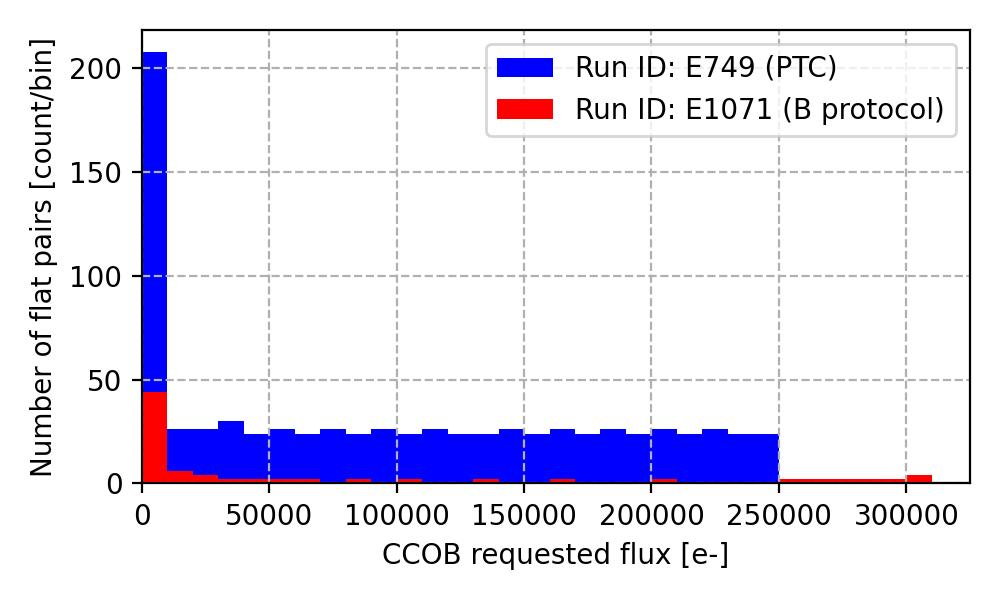
\includegraphics[width=0.9\textwidth]{sections/figures/baselineCharacterization/PTC_BProtocol_Comparison.jpg}
	\caption{Photon Transfer Curve Protocol Comparison
\label{fig:PTC_BProtocol_Comparison}}
\end{centering}
\end{figure}


All EO camera data is processed through the
\href{https://github.com/lsst/cp_pipe}{calibration products} and
\href{https://github.com/lsst-camera-dh/eo_pipe/tree/main}{electro-optical}
pipelines to extract key metrics from the data run. The key camera
metrics from Run 7, and their comparison to previous runs are discussed
below.

The naming of the EO runs was established during initial camera
integration and testing. The final SLAC IR2 run from November 2023 was
named "Run 6", while the data acquisitions from Cerro Pachon are
considered "Run 7." Additionally, individual EO acquisitions are tagged
with a run identifier. This is commonly referred to a Run ID. For all
SLAC runs, the run identifier was a five digit numeric code, while the
Cerro Pachon runs were "E-numbers" that started with a capital E
followed by a numeric code.

For comparison between Cerro Pachon EO runs and the final SLAC IR2, the
following runs are used.

\begin{longtable}[]{@{}
  >{\raggedright\arraybackslash}p{(\linewidth - 4\tabcolsep) * \real{0.1806}}
  >{\raggedright\arraybackslash}p{(\linewidth - 4\tabcolsep) * \real{0.2083}}
  >{\raggedright\arraybackslash}p{(\linewidth - 4\tabcolsep) * \real{0.2639}}@{}}
\toprule\noalign{}
\begin{minipage}[b]{\linewidth}\raggedright
\begin{quote}
Run Type
\end{quote}
\end{minipage} & \begin{minipage}[b]{\linewidth}\raggedright
SLAC IR2 Run
\end{minipage} & \begin{minipage}[b]{\linewidth}\raggedright
Cerro Pachón Run
\end{minipage} \\
\midrule\noalign{}
\endhead
\bottomrule\noalign{}
\endlastfoot
B Protocol & \begin{minipage}[t]{\linewidth}\raggedright
\begin{quote}
13557
\end{quote}
\end{minipage} & \begin{minipage}[t]{\linewidth}\raggedright
\begin{quote}
E1071
\end{quote}
\end{minipage} \\
\begin{minipage}[t]{\linewidth}\raggedright
\begin{quote}
PTC
\end{quote}
\end{minipage} & \begin{minipage}[t]{\linewidth}\raggedright
\begin{quote}
13591
\end{quote}
\end{minipage} & \begin{minipage}[t]{\linewidth}\raggedright
\begin{quote}
E749
\end{quote}
\end{minipage} \\
\end{longtable}

Among all of these measurements, primary concern is that the camera has
maintained its performance standards between the SLAC IR2 run in
November 2023 and the Cerro Pachon run in October 2024.

\subsubsection{Stability flat metrics}\label{stability-flat-metrics}

\paragraph{Charge transfer
inefficiency}\label{charge-transfer-inefficiency}

CTI, or charge transfer inefficiency, measures the fraction of charge
that fails to transfer from the image area to the readout register
during image readout. Consequences of high CTI include loss of charge,
distorted signals in the direction of the parallel register, and reduced
sensitivity in low light imaging. CTI measurements are made using the
EPER method \hyperref[EPER]{{[}EPER{]}}, which compares the ratio of the
residual charge in the overscan pixels to the total signal charge in the
imaging region. In the context of LSSTCam, we measure CTI along both the
serial and parallel registers.

\paragraph{Serial CTI}\label{serial-cti}

\begin{figure}
\begin{centering}
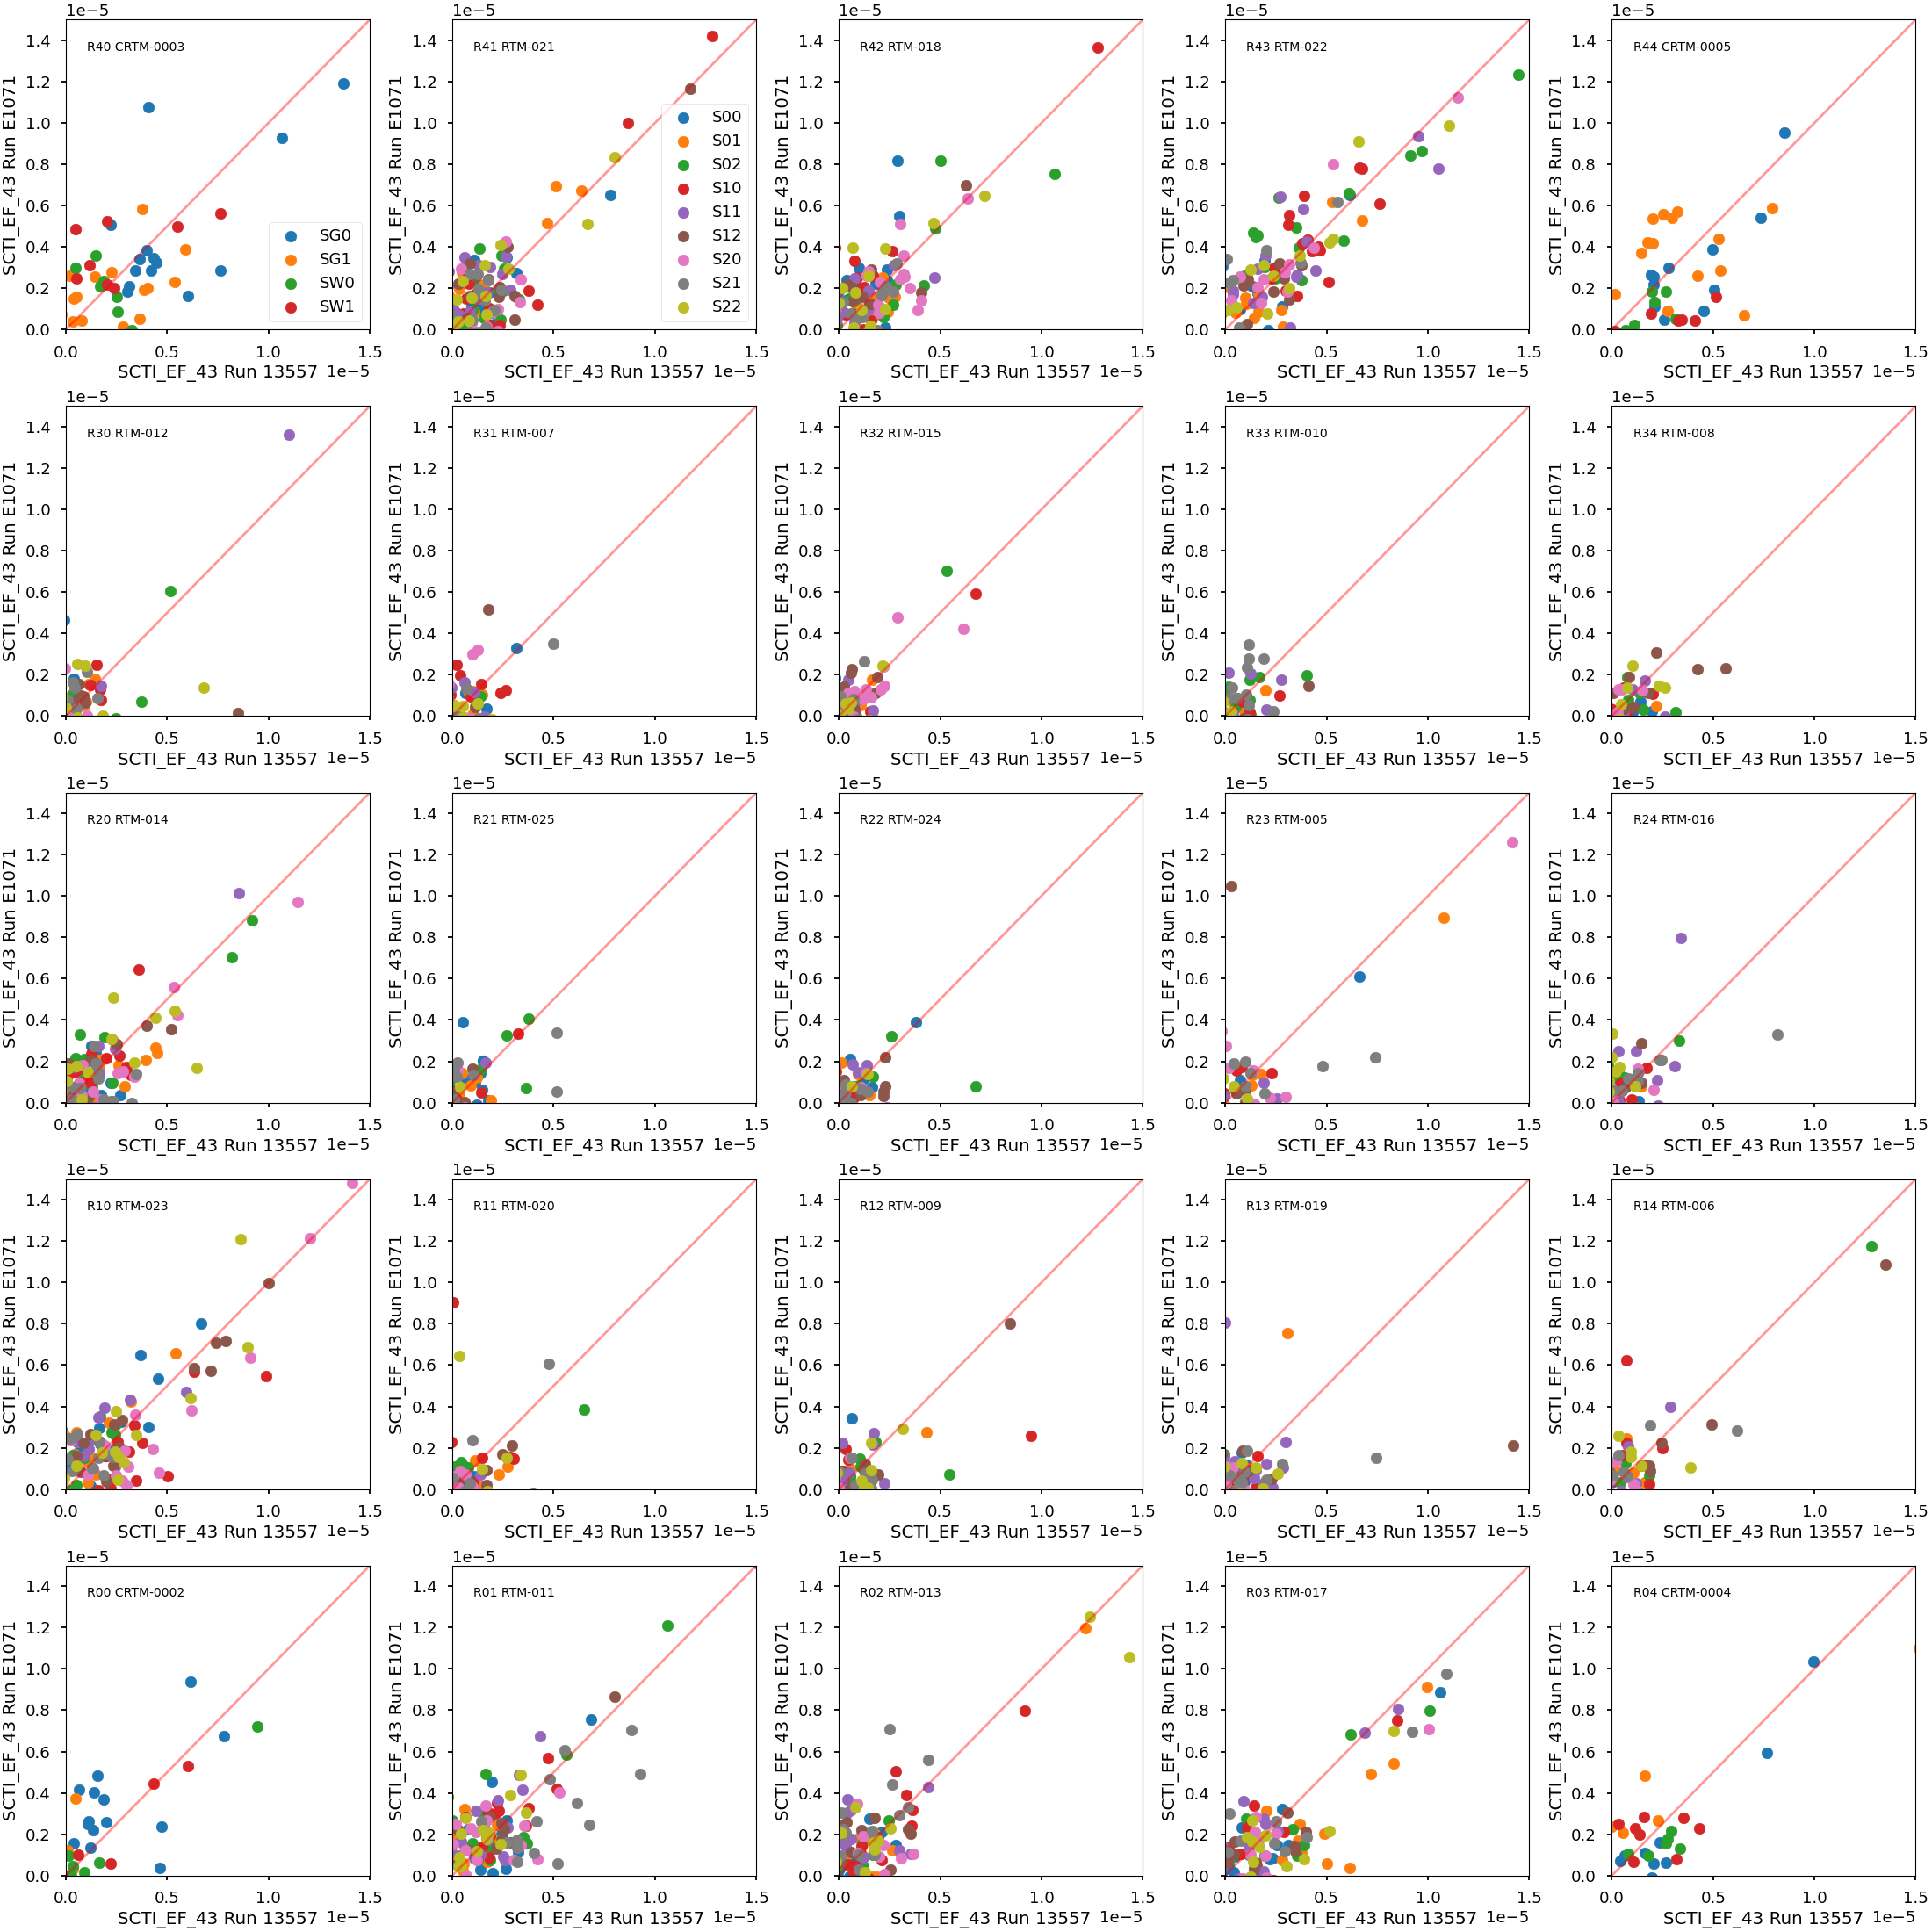
\includegraphics[width=0.9\textwidth]{sections/figures/baselineCharacterization/13557_E1071_SCTI_EF_43.png}
	\caption{Serial CTI \label{fig:serial-cti}}
\end{centering}
\end{figure}

The CTI along the serial register is consistent between both Run 6 and
Run 7. Both sensor types show extremely low CTI on the order of 1E-3 \%,
and differ on the order of \textasciitilde2E-5 \% for E2V sensors, and
by \textasciitilde4E-6 \% for ITL sensors.

\begin{figure}
\begin{centering}
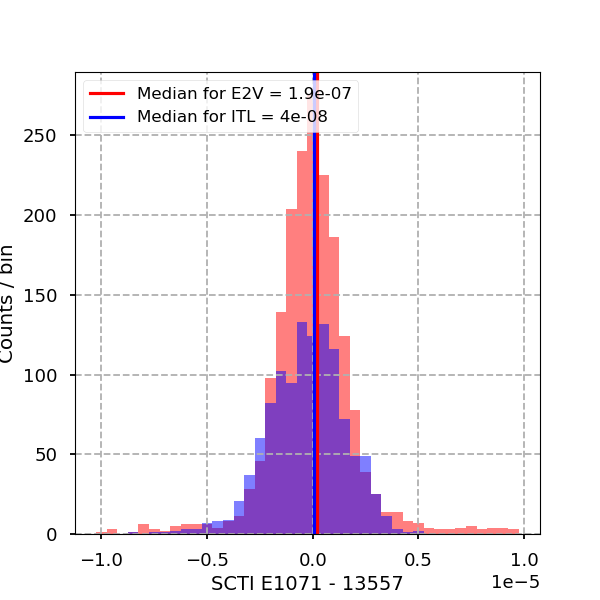
\includegraphics[width=0.9\textwidth]{sections/figures/baselineCharacterization/SCTI_13557_E1071_diff.png}
\end{centering}
\end{figure}

\paragraph{Parallel CTI}\label{parallel-cti}

\begin{figure}
\begin{centering}
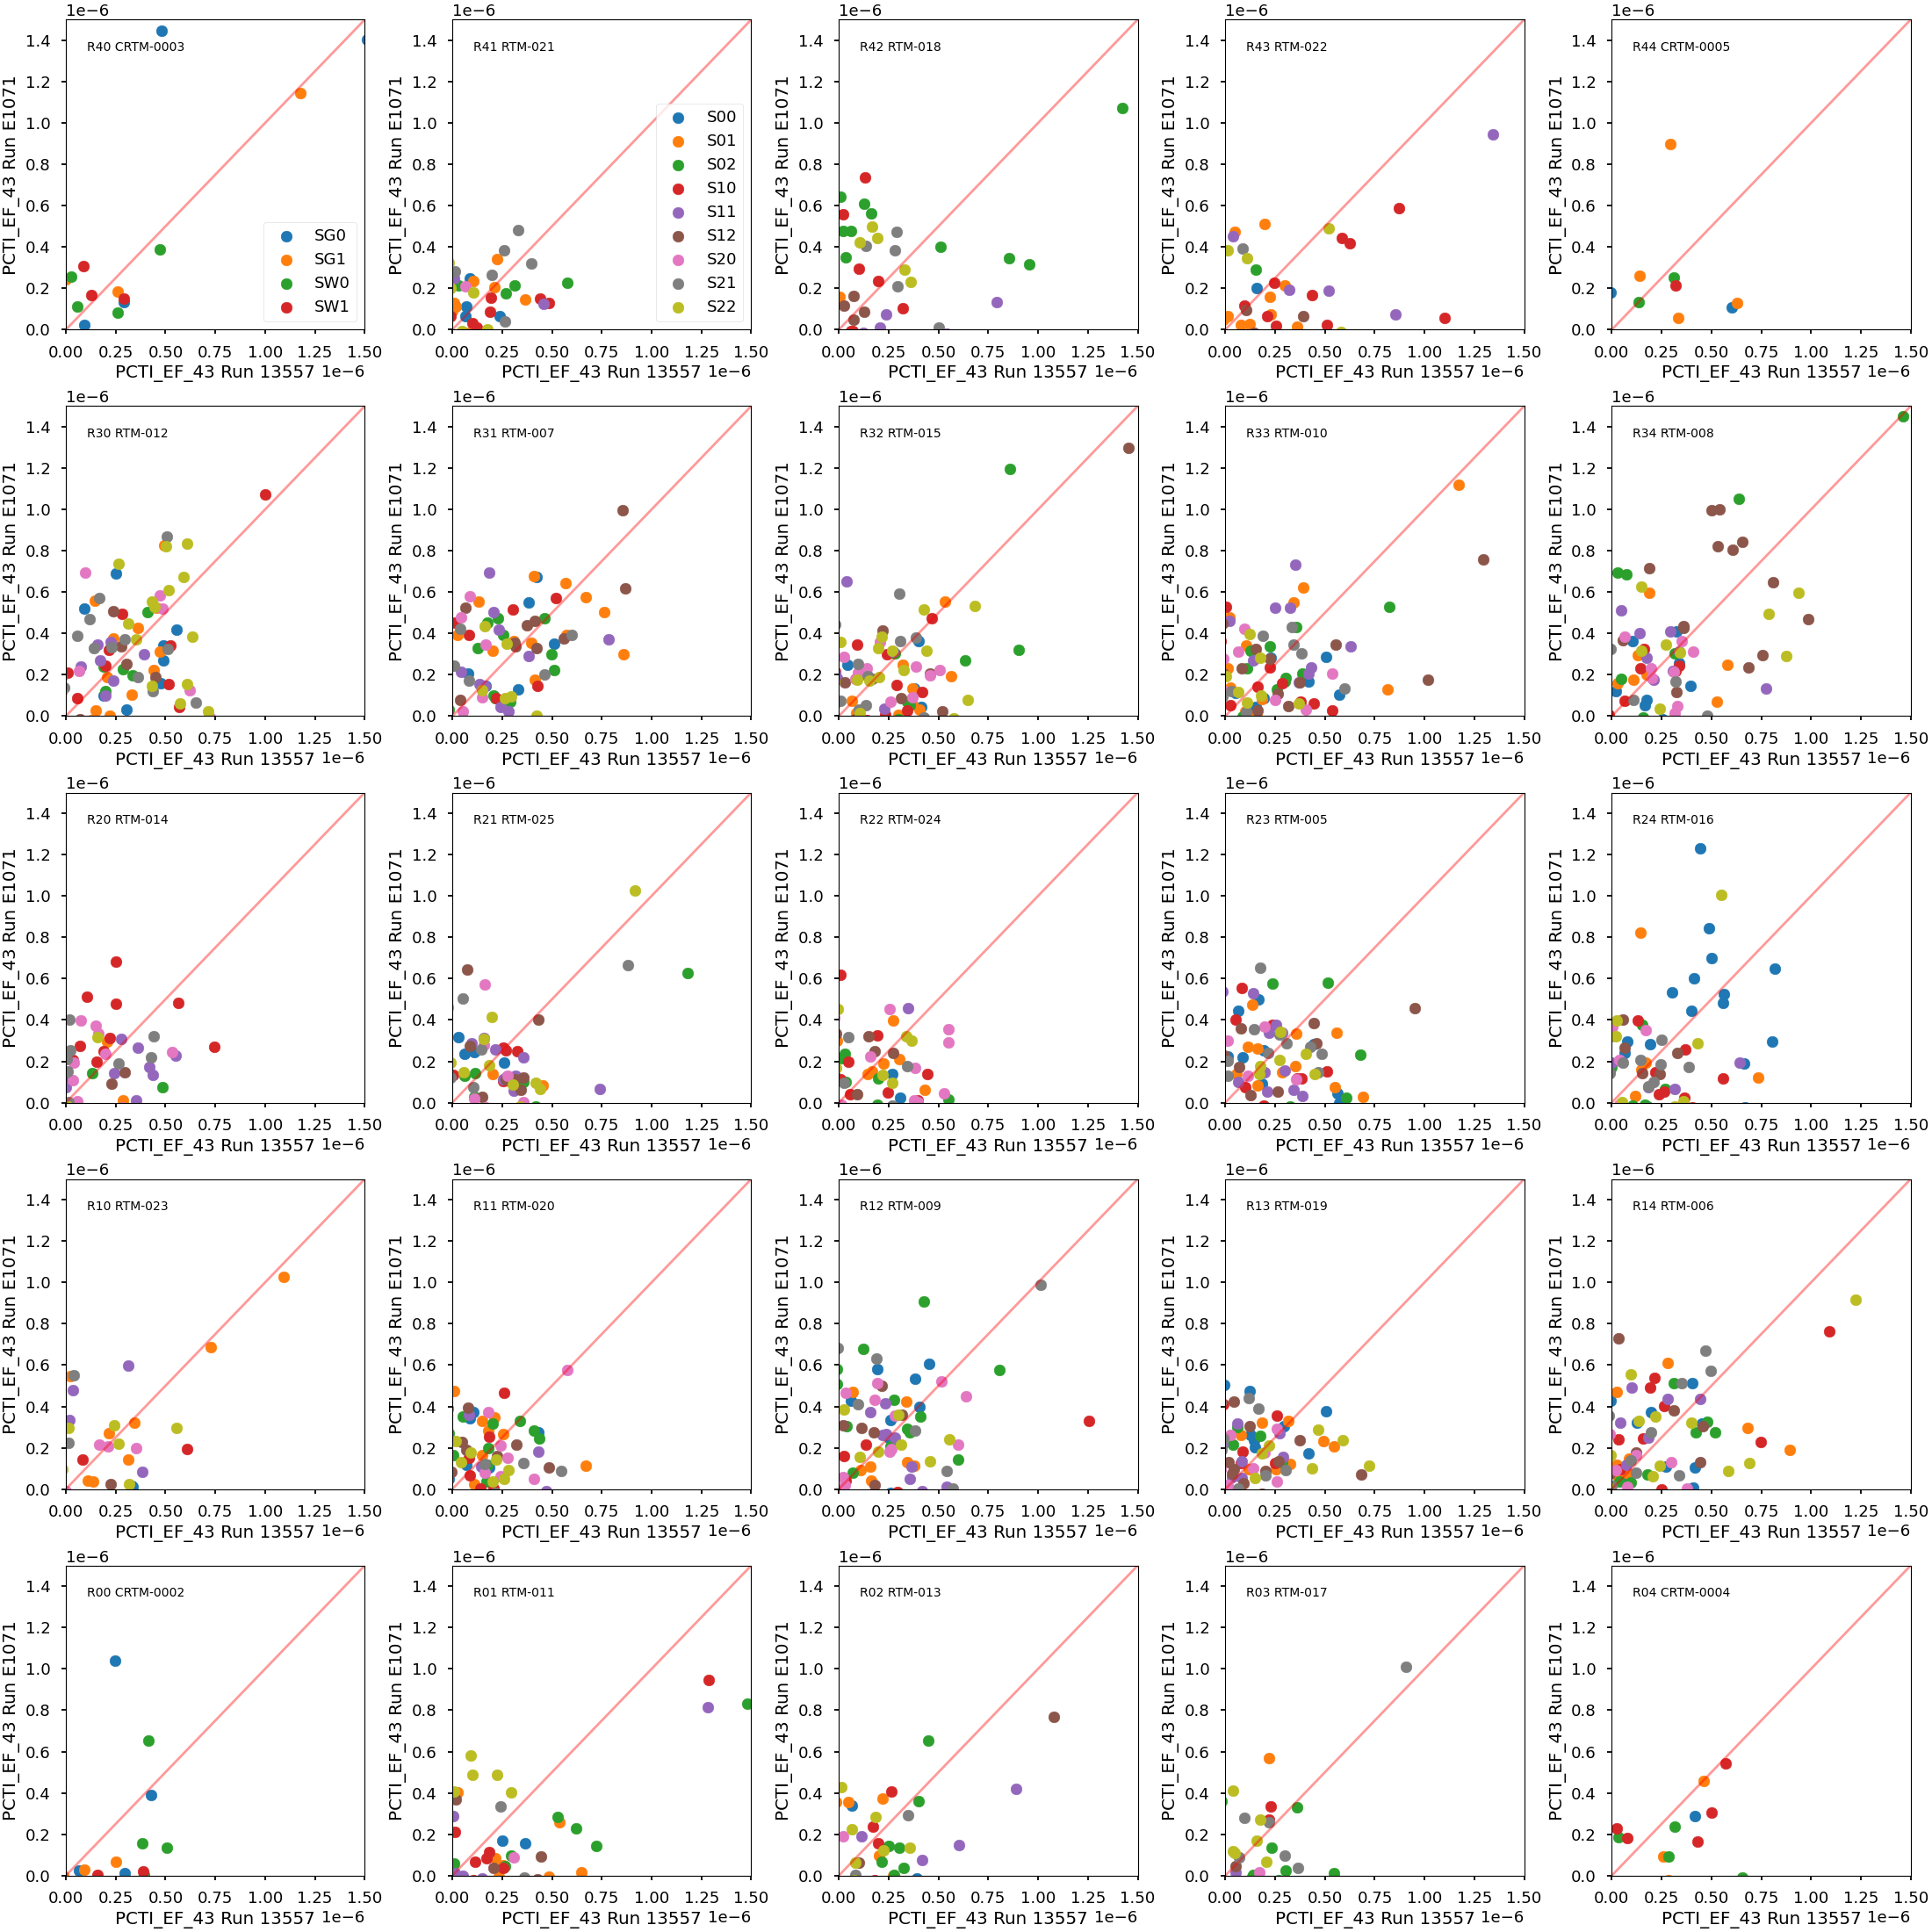
\includegraphics[width=0.9\textwidth]{sections/figures/baselineCharacterization/13557_E1071_PCTI_EF_43.png}
\end{centering}
\end{figure}

The CTI along the parallel register is consistent between both Run 6 and
Run 7. Both sensor types show extremely low CTI on the order of 1E-5 \%,
and differ on the order of \textasciitilde2E-7 \% for E2V sensors, and
by \textasciitilde7E-6 \% for ITL sensors.

\begin{figure}
\begin{centering}
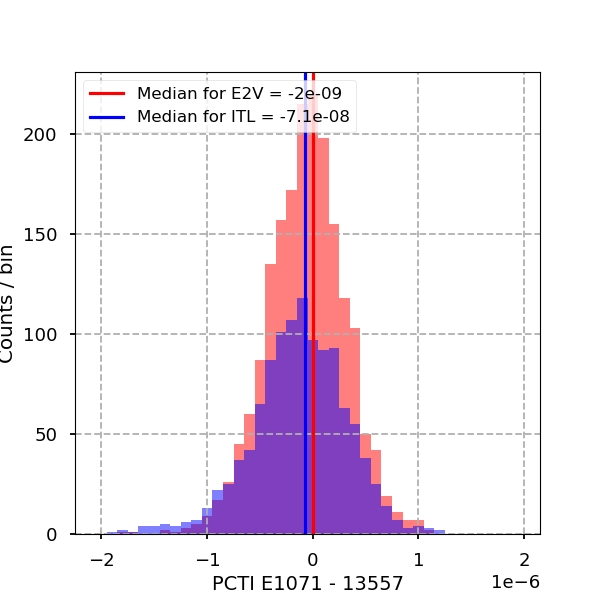
\includegraphics[width=0.9\textwidth]{sections/figures/baselineCharacterization/PCTI_13557_E1071_diff.png}
\end{centering}
\end{figure}

\subsubsection{Dark metrics}\label{dark-metrics}

\paragraph{Dark current}\label{dark-current}

Dark current is the small amount of electrical charge generated in the
absence of light due to thermal activity within the CCD's semiconductor
material. This effect occurs when thermal energy causes electrons to be
released from atoms in the CCD, mimicking the signal that light would
produce. Dark current increases with temperature, so cooling the CCD is
a common method to reduce it in sensitive imaging applications. Dark
current introduces noise into an image, degrading its quality,
particularly in low-light conditions or long exposures. In the context
of LSSTCam, we measure dark current from the combined dark images across
all amplifiers.

\begin{figure}
\begin{centering}
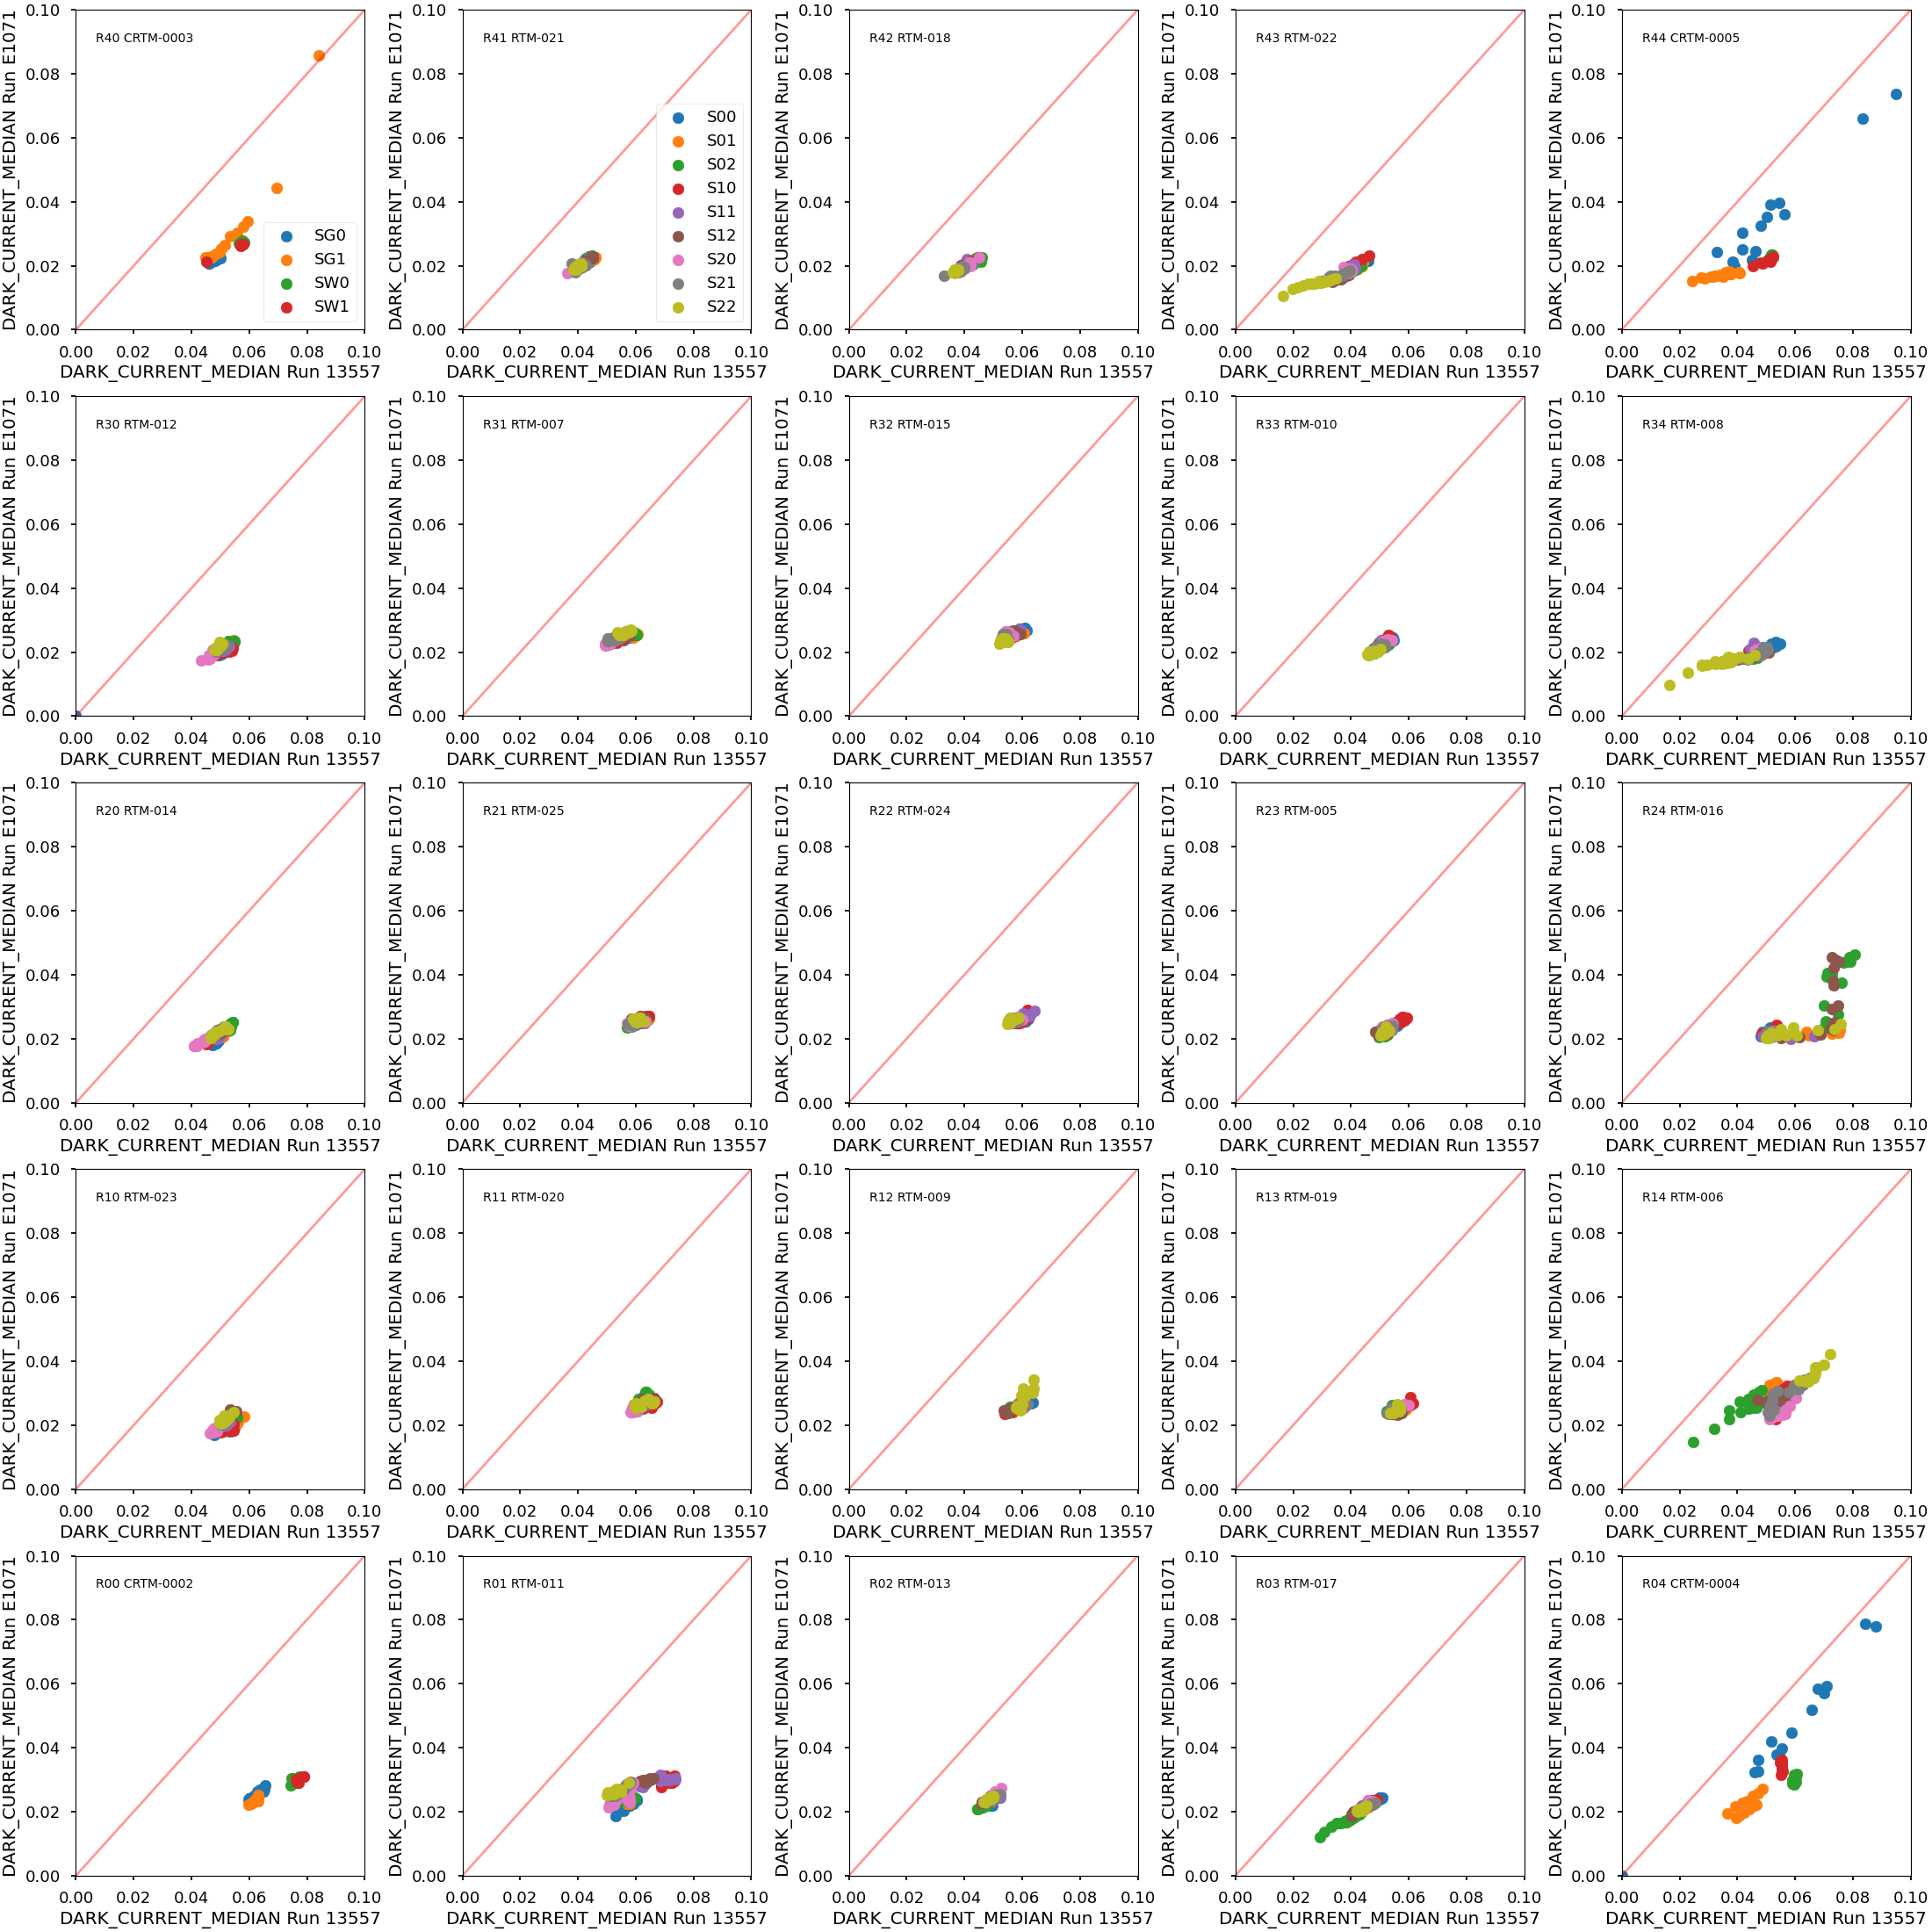
\includegraphics[width=0.9\textwidth]{sections/figures/baselineCharacterization/13557_E1071_DARK_CURRENT_MEDIAN.png}
\end{centering}
\end{figure}

Surprisingly, dark current was significantly lowered in Run 7 compared
to run 6. Possible reasons for this could be improved shrouding
conditions on the camera on Cerro Pachon compared to SLAC.

\paragraph{Bright defects}\label{bright-defects}

Bright defects are localized regions or individual pixels that produce
abnormally high signal levels, even in the absence of light. These
defects are typically caused by imperfections in the CCD's semiconductor
material or manufacturing process. Bright defects can manifest as ``hot
pixelspixels with consistently high dark current), small clusters of
pixels with elevated output, or as "hot columns" (pixels along the same
parallel register that have high dark current). In the context of
LSSTCam, we extract bright pixels from the dark current, with the
threshold for a bright defect set at 5 e- / pix / s, above which the
pixel is registered as a bright defect.

\begin{figure}
\begin{centering}
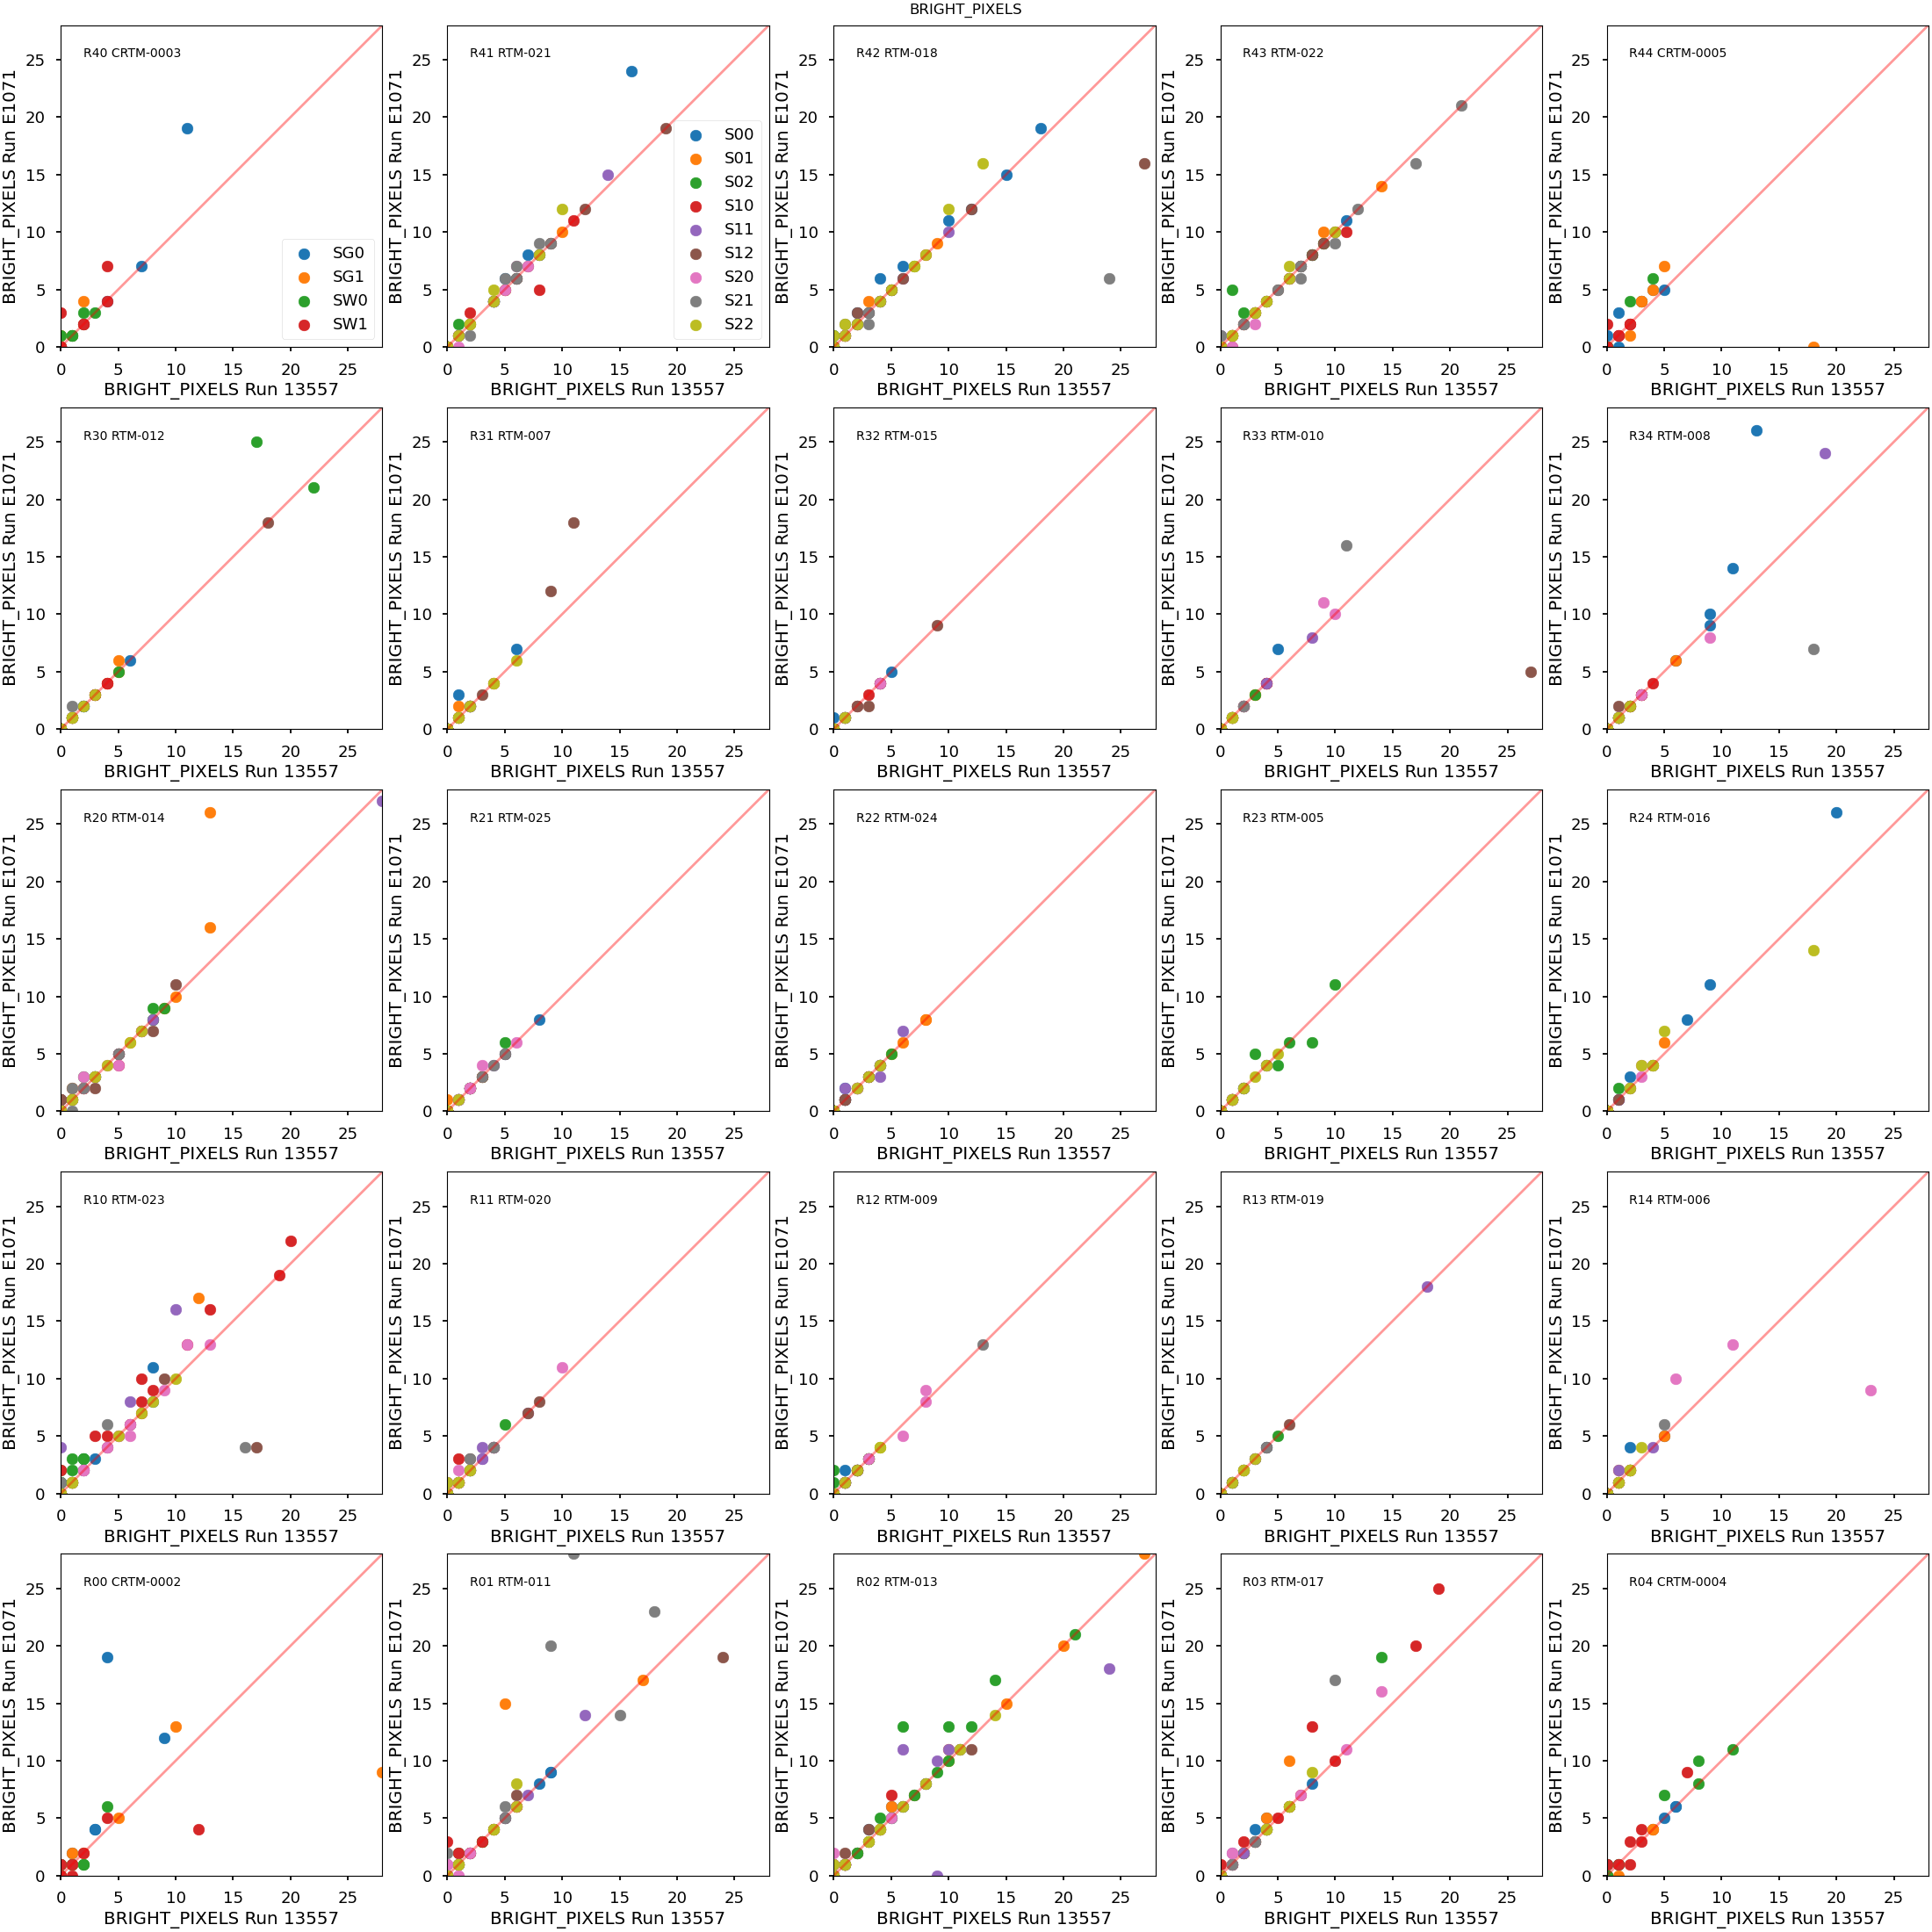
\includegraphics[width=0.9\textwidth]{sections/figures/baselineCharacterization/13557_E1071_BRIGHT_PIXELS.png}
\end{centering}
\end{figure}

Reviewing the differences in bright pixels, we find consistent bright
defect counts between Run 6 and Run 7. There appears to be a small
excess of bright defects in Run 7.

\begin{figure}
\begin{centering}
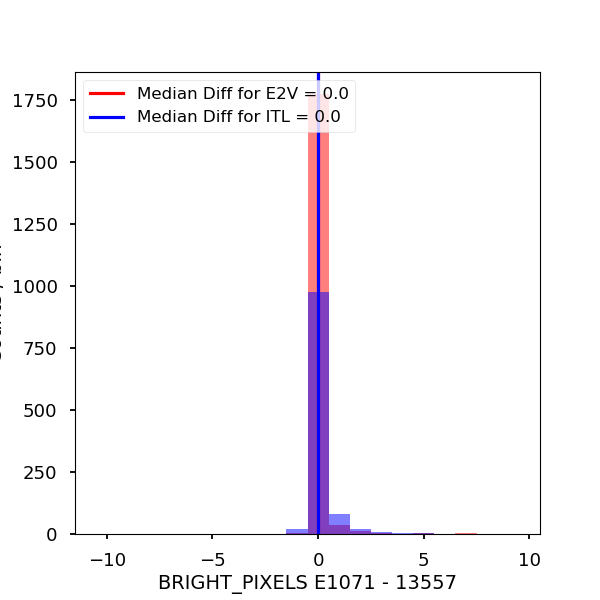
\includegraphics[width=0.9\textwidth]{sections/figures/baselineCharacterization/BRIGHT_PIXELS_13557_E1071_diff.png}
\end{centering}
\end{figure}

Taking the difference of defect counts on each amplifier, and separating
the amplifiers by the detector manufacturer shows a small excess of
bright defects in run 7 when compared to run 6. For ITL sensors, we find
12\% of the amplifiers with more bright pixels than run 6. For E2V
sensors, we find 4\% of the amplifiers with more bright pixels than run
6. Despite this, the number of bright defects between runs does not
increase for most sensors.

\subsubsection{Flat pair metrics}\label{flat-pair-metrics}

\begin{figure}
\begin{centering}
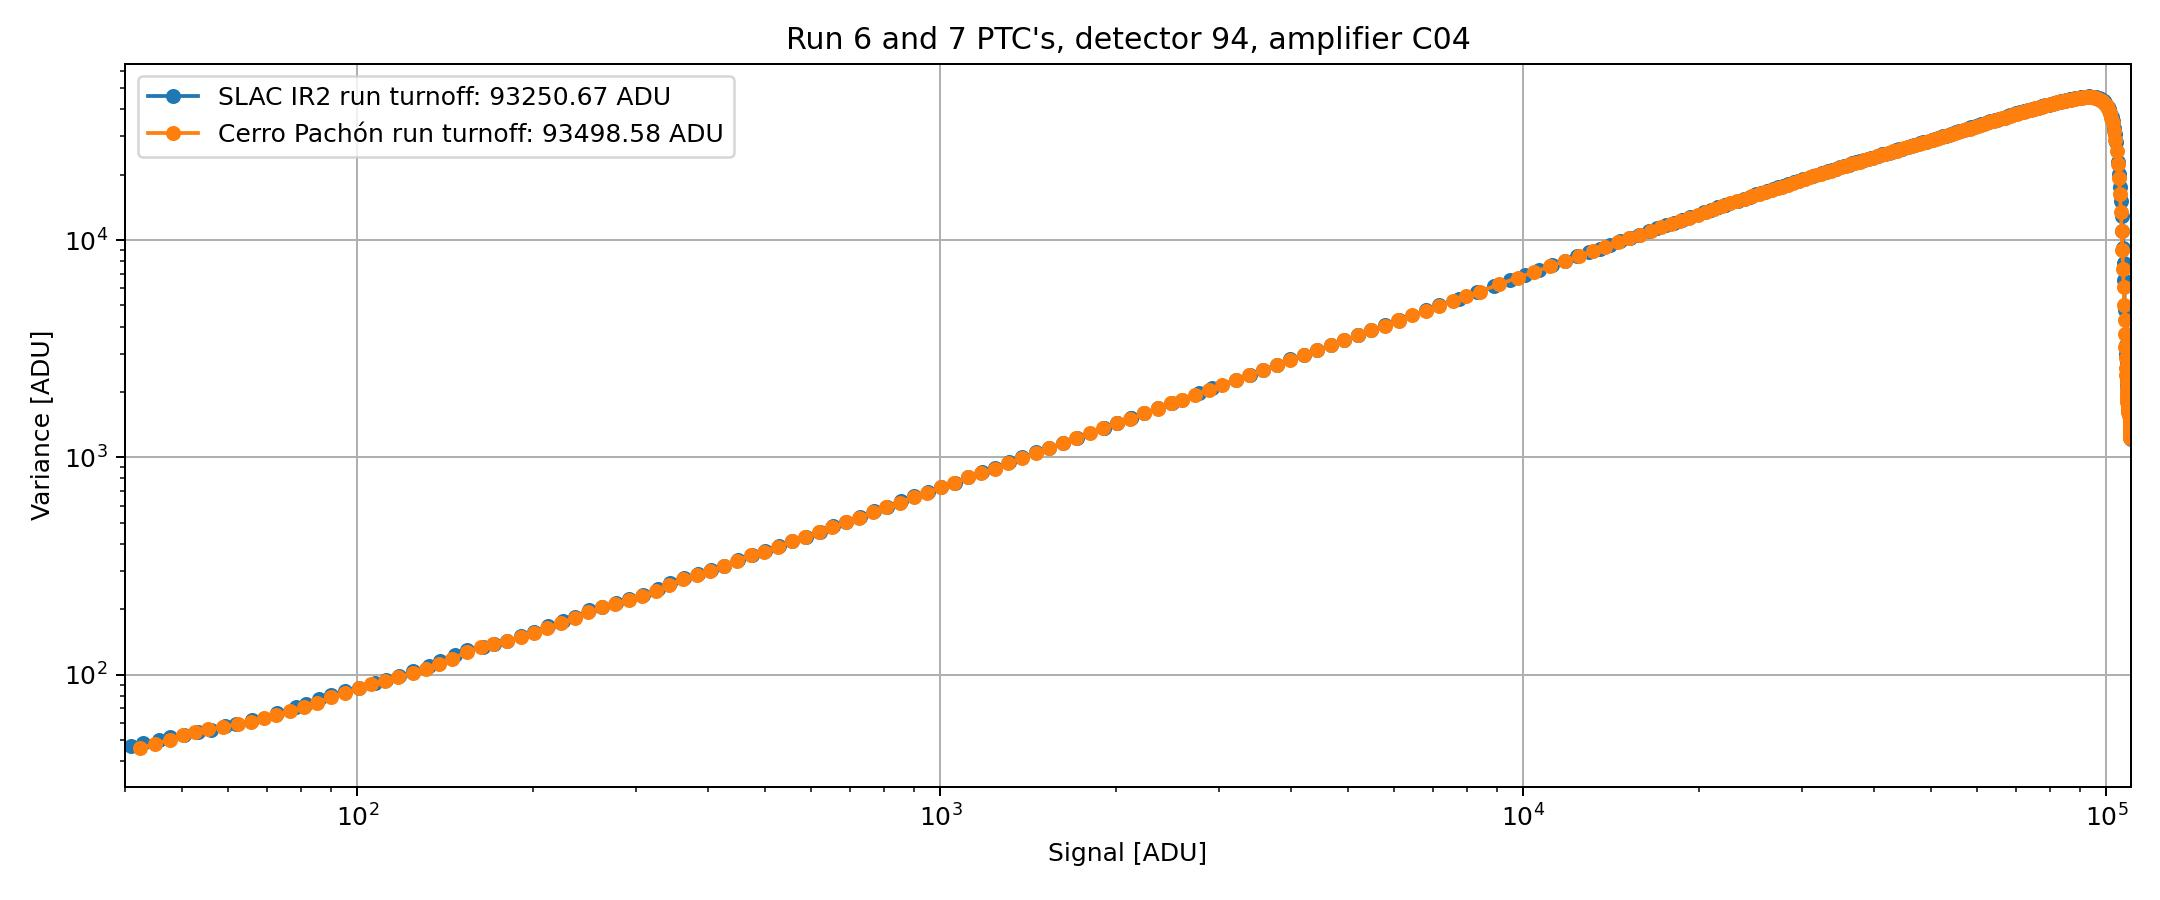
\includegraphics[width=0.9\textwidth]{sections/figures/baselineCharacterization/run7PTCsToDate.jpg}
\end{centering}
\end{figure}

\paragraph{Linearity and PTC turnoff}\label{linearity-and-ptc-turnoff}

Linearity turnoff and PTC turnoff are two closely related metrics used
to characterize the upper limit of the usable signal range for accurate
imaging. Linearity turnoff is the point at which LSSTCam deviates from
linearity in the PTC curve. In our case, the deviation threshold is 2\%.
PTC turnoff refers to the high signal region of the PTC where the PTC
begins to decrease noise for higher flux. This is due to blooming and
saturation within the CCDs. While slightly different, both metrics
provide important information about the upper limits of the dynamic
range in our sensors. Linearity turnoff is measured in units of e-,
while PTC turnoff is measured in ADU.

\begin{figure}
\begin{centering}
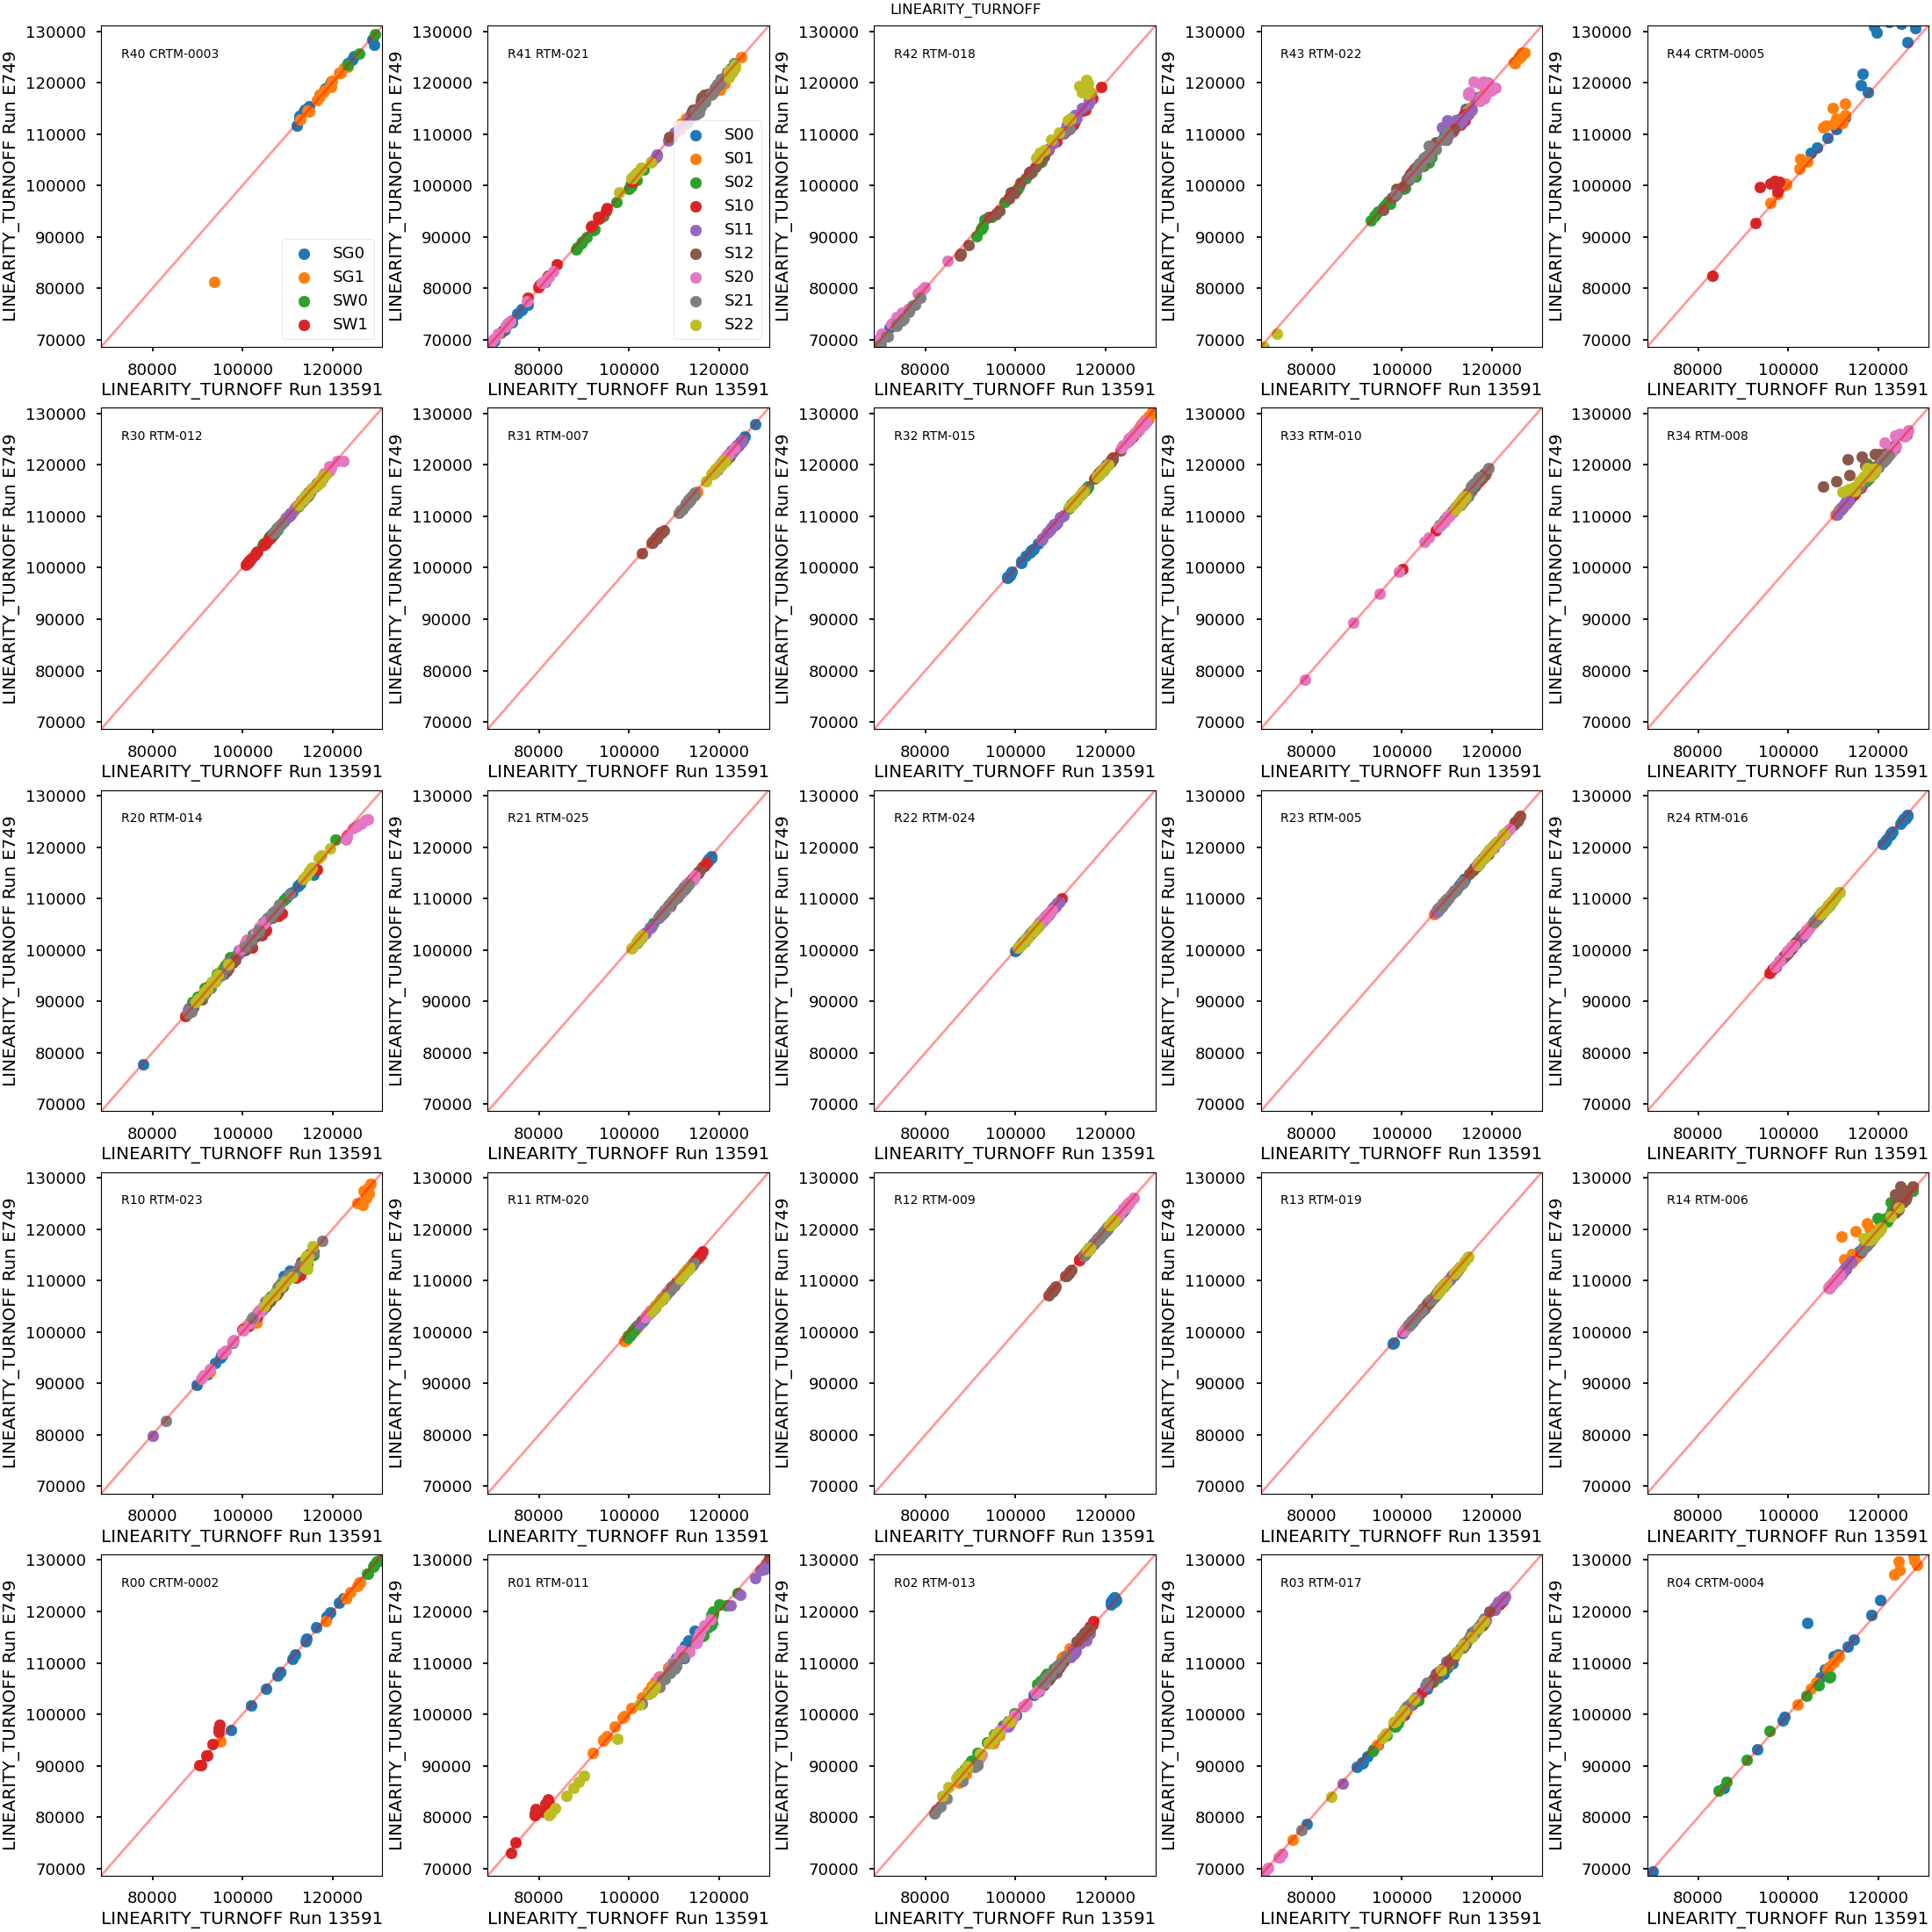
\includegraphics[width=0.9\textwidth]{sections/figures/baselineCharacterization/13591_E749_LINEARITY_TURNOFF.png}
\end{centering}
\end{figure}

In our linearity turnoff measurements, we find close agreement between
our Run 7 and Run 6 measurements. Both ITL and E2V sensors show tight
agreement between results.

\begin{figure}
\begin{centering}
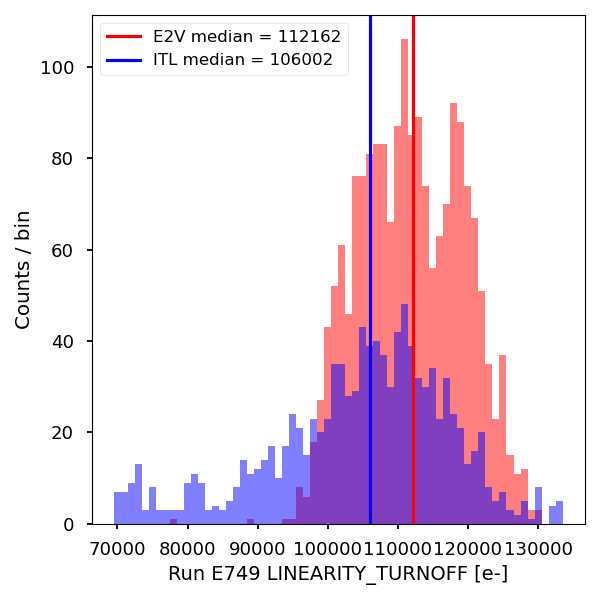
\includegraphics[width=0.9\textwidth]{sections/figures/baselineCharacterization/LINEARITY_TURNOFF_E749_sensorType.png}
\end{centering}
\end{figure}

\paragraph{PTC Gain}\label{ptc-gain}

PTC gain is the conversion factor between the number of electrons
generated in the CCD\textquotesingle s pixels and the digital output
signal. It is one of the key parameters derived from the Photon Transfer
Curve, as it is the slope from where the noise is dominated by shot
noise. Gain is expressed in e- / ADU, and quantifies how effective the
CCD\textquotesingle s analog signal is digitized.

\begin{figure}
\begin{centering}
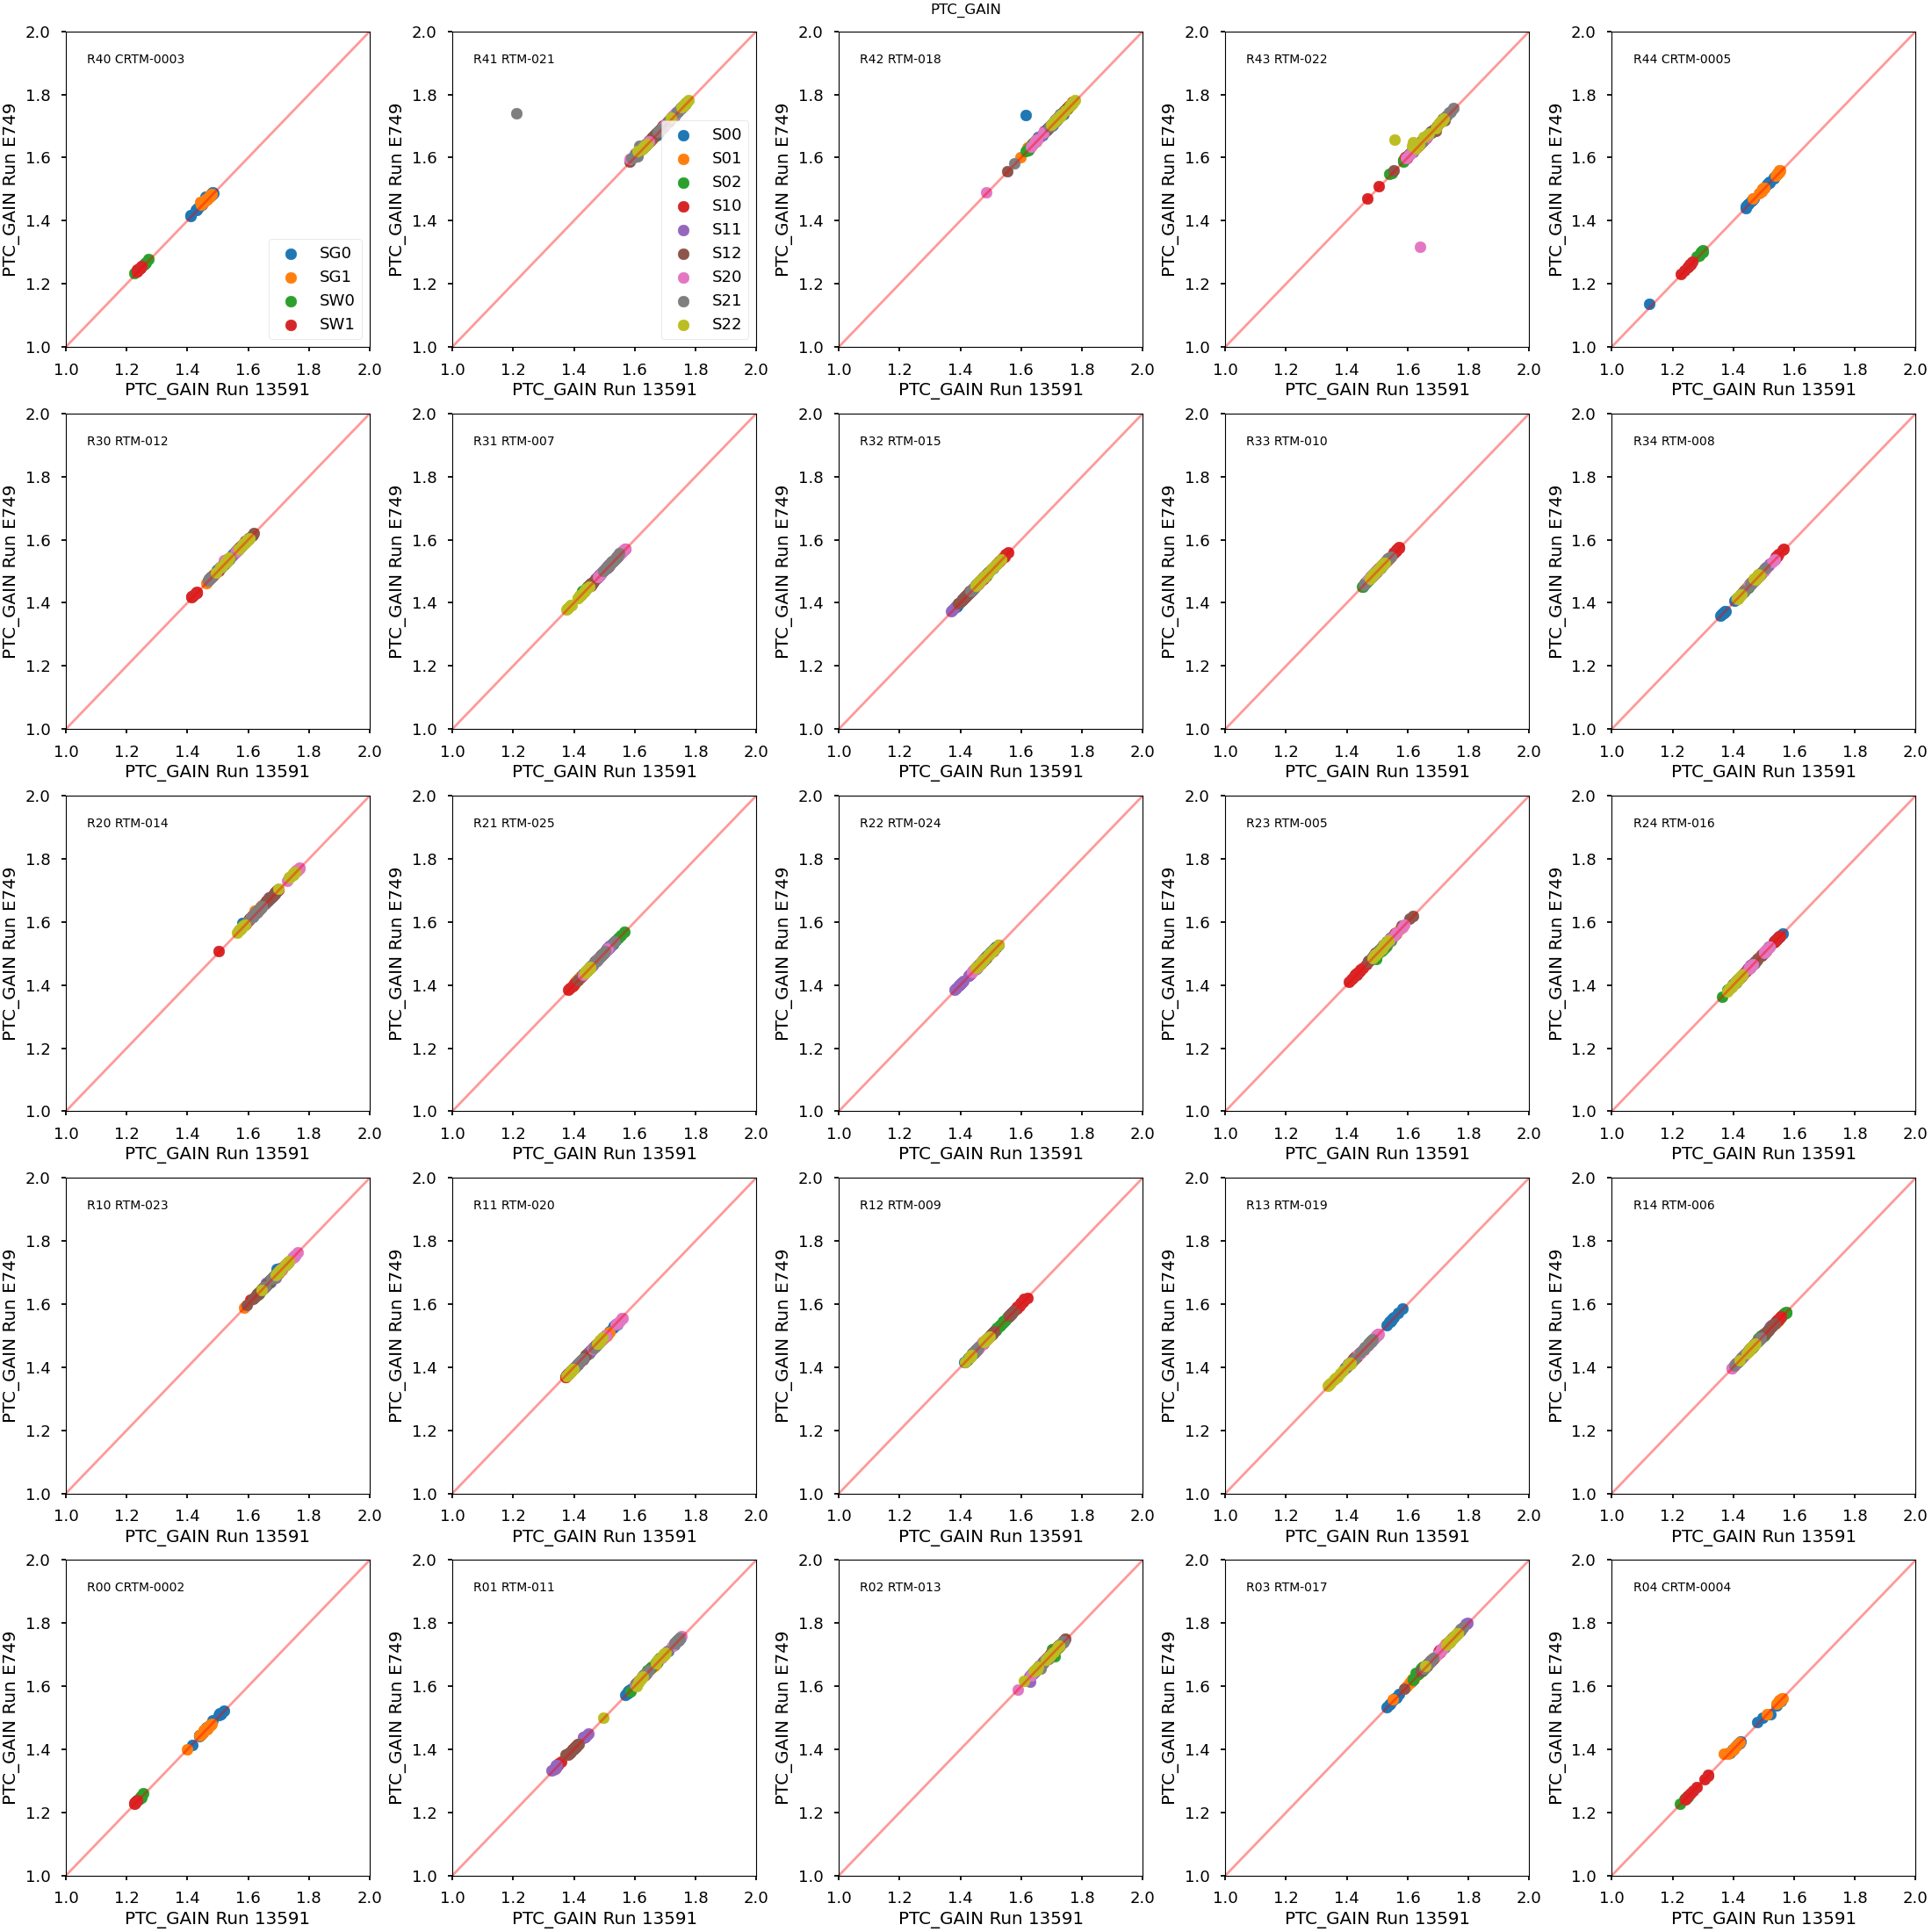
\includegraphics[width=0.9\textwidth]{sections/figures/baselineCharacterization/13591_E749_PTC_GAIN.png}
\end{centering}
\end{figure}

PTC gain measurements agree extremely closely across all sensors in the
focal plane.

\paragraph{\texorpdfstring{Brighter fatter a{00}
coefficient}{Brighter fatter a00 coefficient}}\label{brighter-fatter-a00-coefficient}

This redistribution causes the charge to ``spillnto adjacent pixels,
effectively broadening the point spread function (PSF). The brighter
fatter effect is the most dominant source of variance in the PTC curve.
The brighter-fatter effect in CCDs refers to the phenomenon where
brighter pixels appear larger (or ``fatterthan dimmer ones. This occurs
due to electrostatic interactions within the CCD, when a pixel
accumulates a high charge from incoming photons and creates an electric
field that slightly repels incoming charge carriers into neighboring
pixels. The brighter fatter effect can be modeled as the most dominant
source of pixel-pixel correlations. Following the PTC model from
\hyperref[Astier]{{[}Astier{]}}, a00 describes the change of a pixel
area due to its own charge content, or the relative strength of the
brighter-fatter effect. Since same-charge carriers repel each other,
this pixel area has to shrink as charge accumulates inside the pixel,
which implies a00 \textless{} 0. In eo\phantomsection\label{pipe}{pipe},
an absolute value is taken of the a{00} parameter, so the measurements
appear positive.

\begin{figure}
\begin{centering}
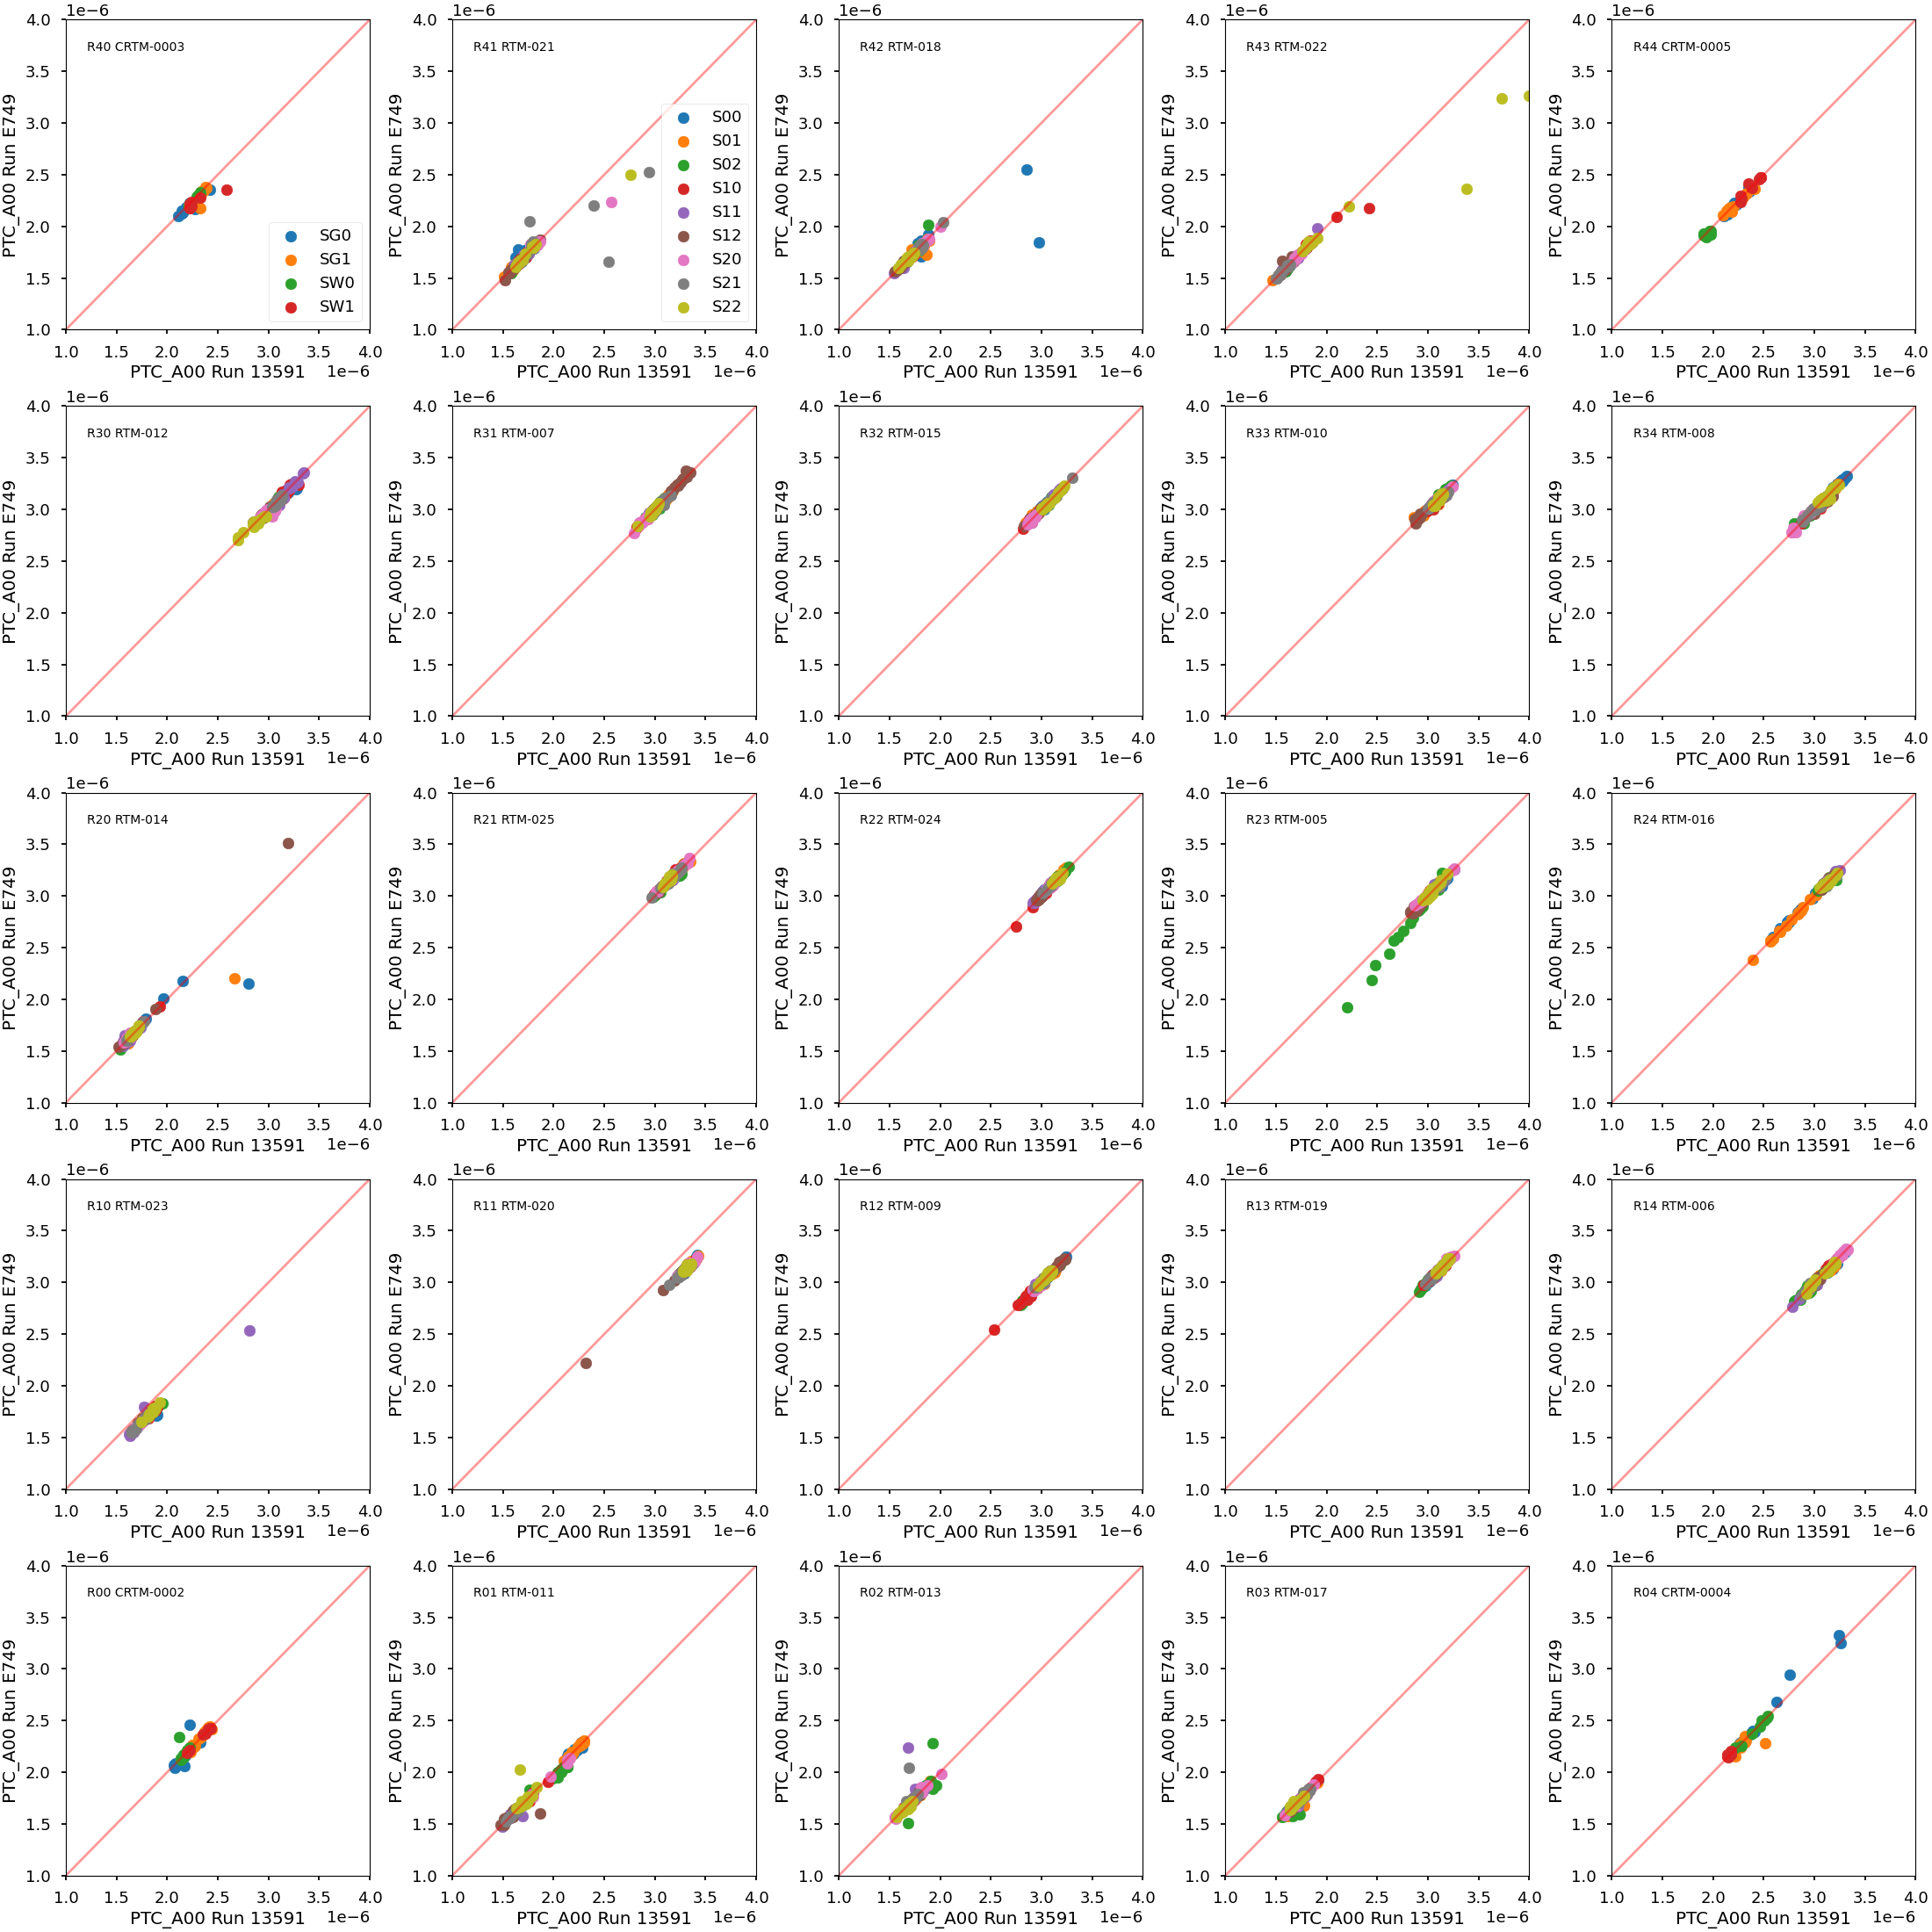
\includegraphics[width=0.9\textwidth]{sections/figures/baselineCharacterization/13591_E749_PTC_A00.png}
\end{centering}
\end{figure}

Comparing the results on the strength of the brighter fatter effect,
both runs are generally comparable. A few outliers exist across the
focal plane, regardless of detector type.

\begin{figure}
\begin{centering}
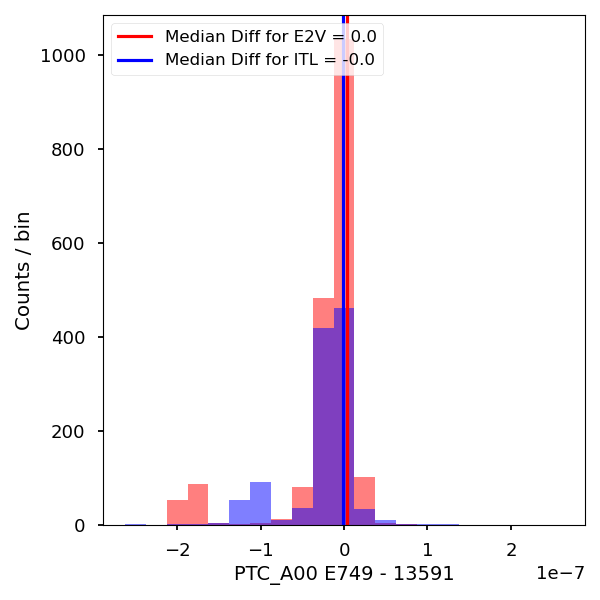
\includegraphics[width=0.9\textwidth]{sections/figures/baselineCharacterization/PTC_A00_13591_E749_diff.png}
\end{centering}
\end{figure}

However, the differences in brighter fatter strength between run 6 and
run 7 show that the strength of the A{00} coefficient decreased for most
of our outliers, which implies an improvement in focal-plane performance

\paragraph{Divisadero Tearing}\label{divisadero-tearing}

Divisadero tearing are large signal variations at amplifier boundaries.
To quantify divisadero tearing, we measure the column signal, and
compare it to the mean column signal from flat fields to quantify the
amplitude of the effect, measured in a percent variation relative to the
mean column signal value.

\begin{figure}
\begin{centering}
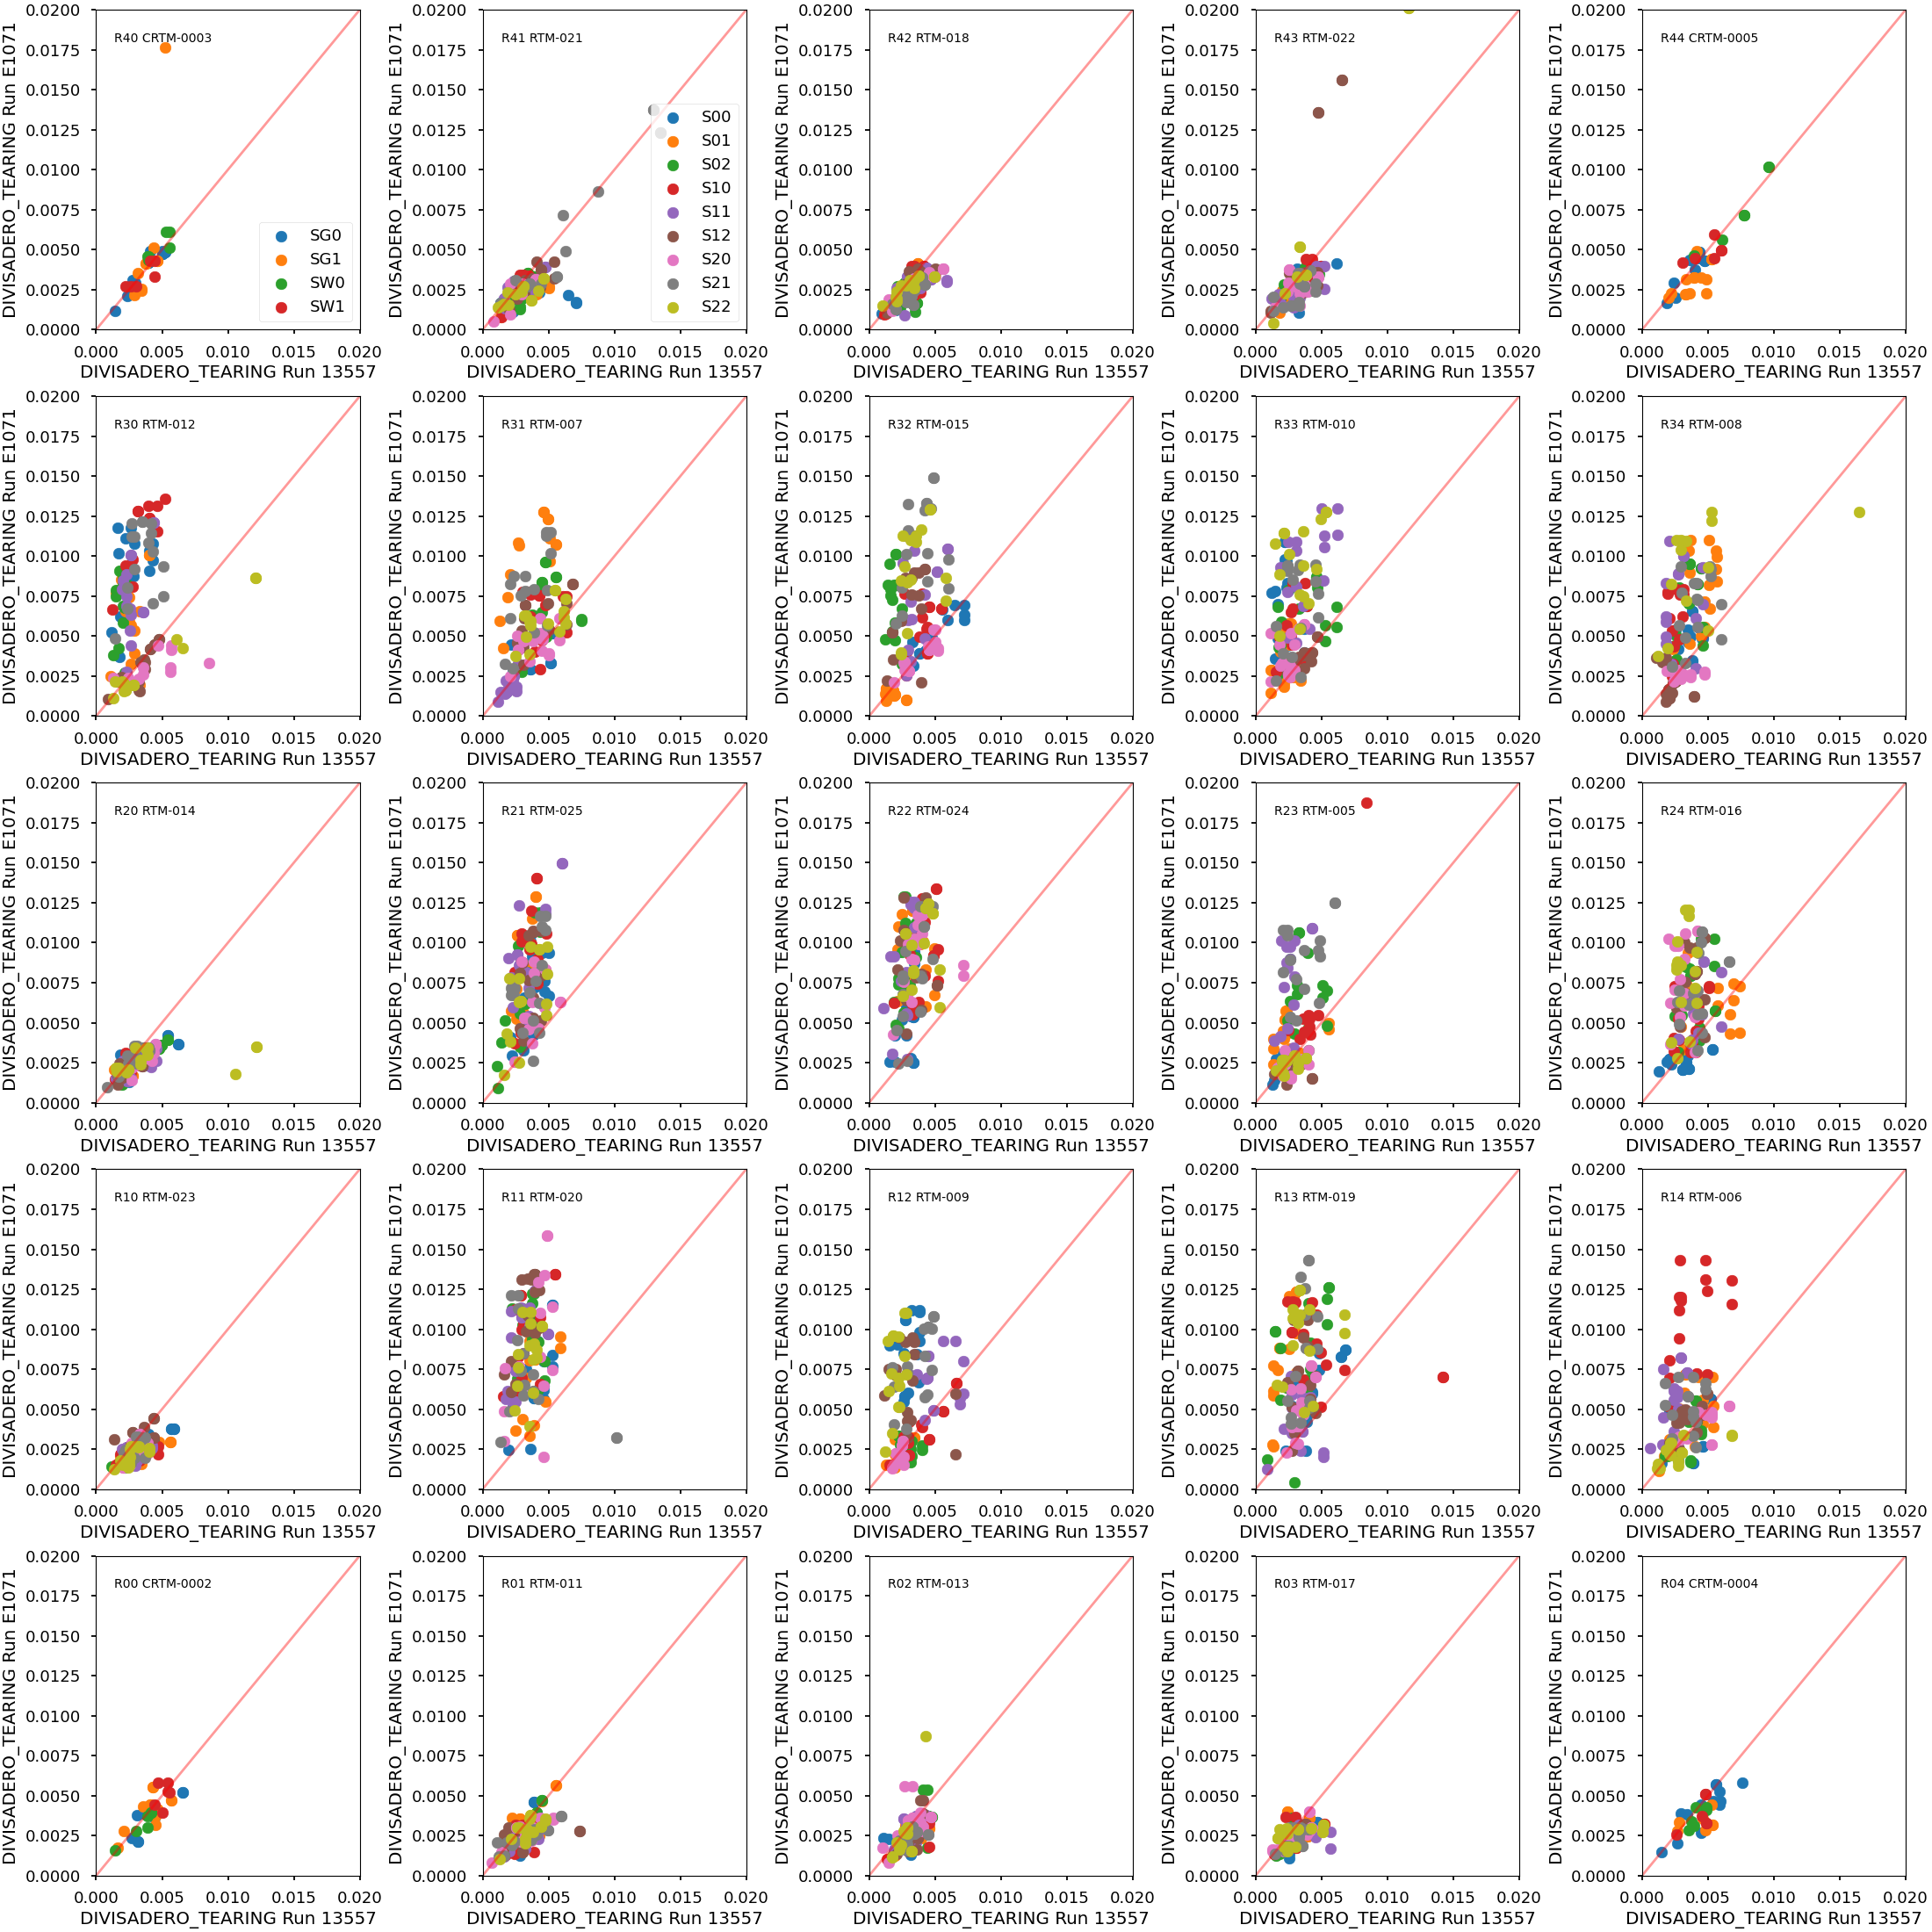
\includegraphics[width=0.9\textwidth]{sections/figures/baselineCharacterization/13557_E1071_DIVISADERO_TEARING.png}
\end{centering}
\end{figure}

Divisadero tearing in E2V CCDs appears higher in Run 7 than Run 6. ITL
sensors are very consistent between runs.

\begin{figure}
\begin{centering}
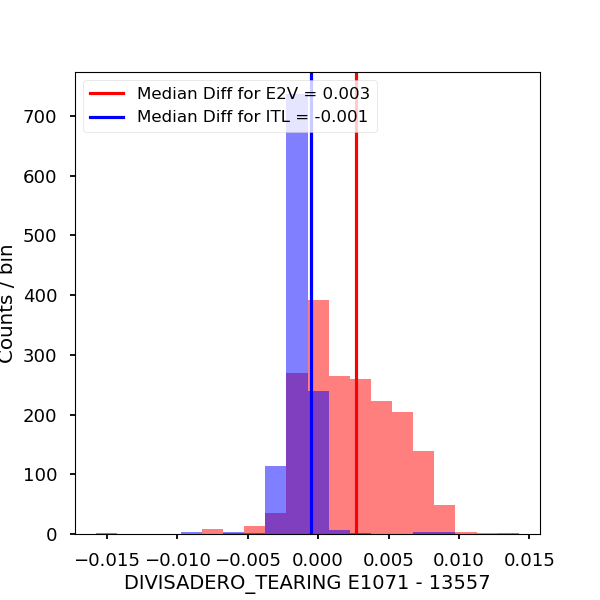
\includegraphics[width=0.9\textwidth]{sections/figures/baselineCharacterization/DIVISADERO_TEARING_13557_E1071_diff.png}
\end{centering}
\end{figure}

Run 7 shows a \textasciitilde0.3\% excess in divisadero tearing for E2V
sensors, compared to an excess of \textasciitilde0.1\% excess in run 6
divisadero tearing for ITL sensors.

\paragraph{Dark defects}\label{dark-defects}

Dark defects are localized regions or individual pixels that produce
abnormally low signal levels, even in the presence of light. These
defects are typically caused by imperfections in the CCD's semiconductor
material or manufacturing process. In the context of LSSTCam, we extract
dark pixels from combined flats, with the threshold for a dark defect
set to a 20\% deviation from flatness.

\begin{figure}
\begin{centering}
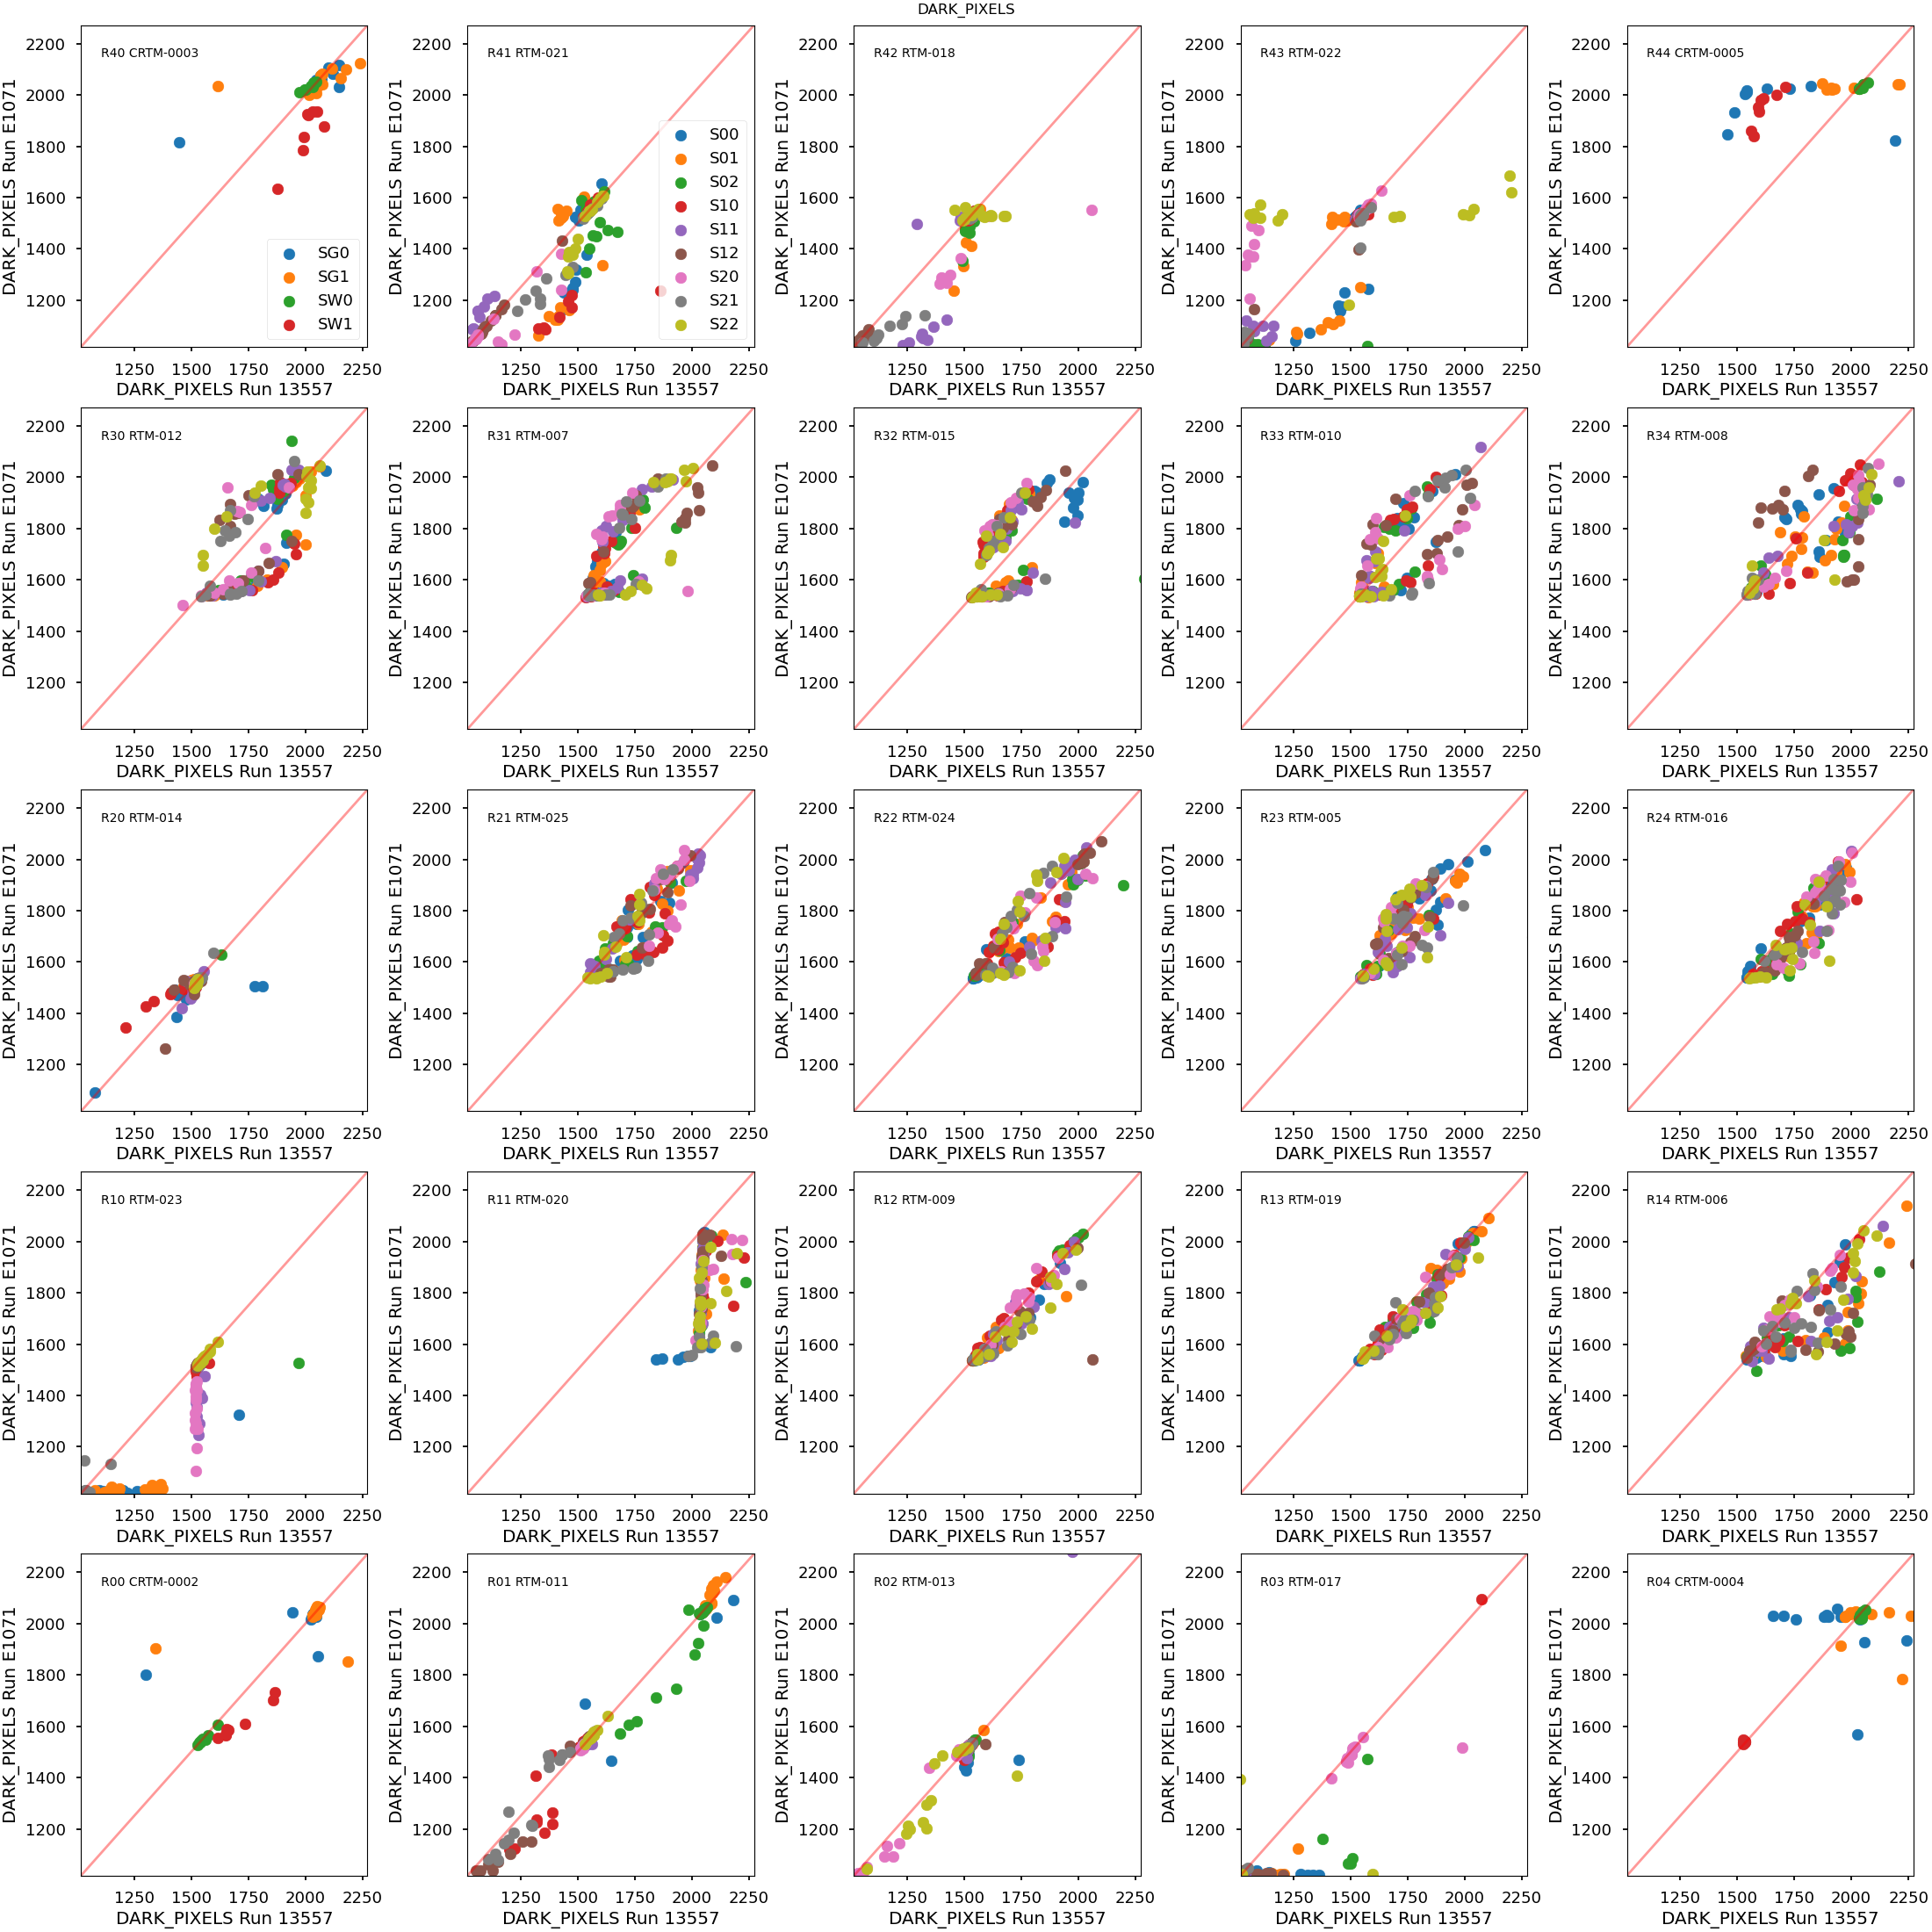
\includegraphics[width=0.9\textwidth]{sections/figures/baselineCharacterization/13557_E1071_DARK_PIXELS.png}
\end{centering}
\end{figure}

Dark pixels measures between SLAC and Cerro Pachon average
\textasciitilde1800 per amplifier, regardless of manufacturer. The
reason for the high dark pixel counts is due to a picture-frame response
near the edges of the sensors.

\begin{figure}
\begin{centering}
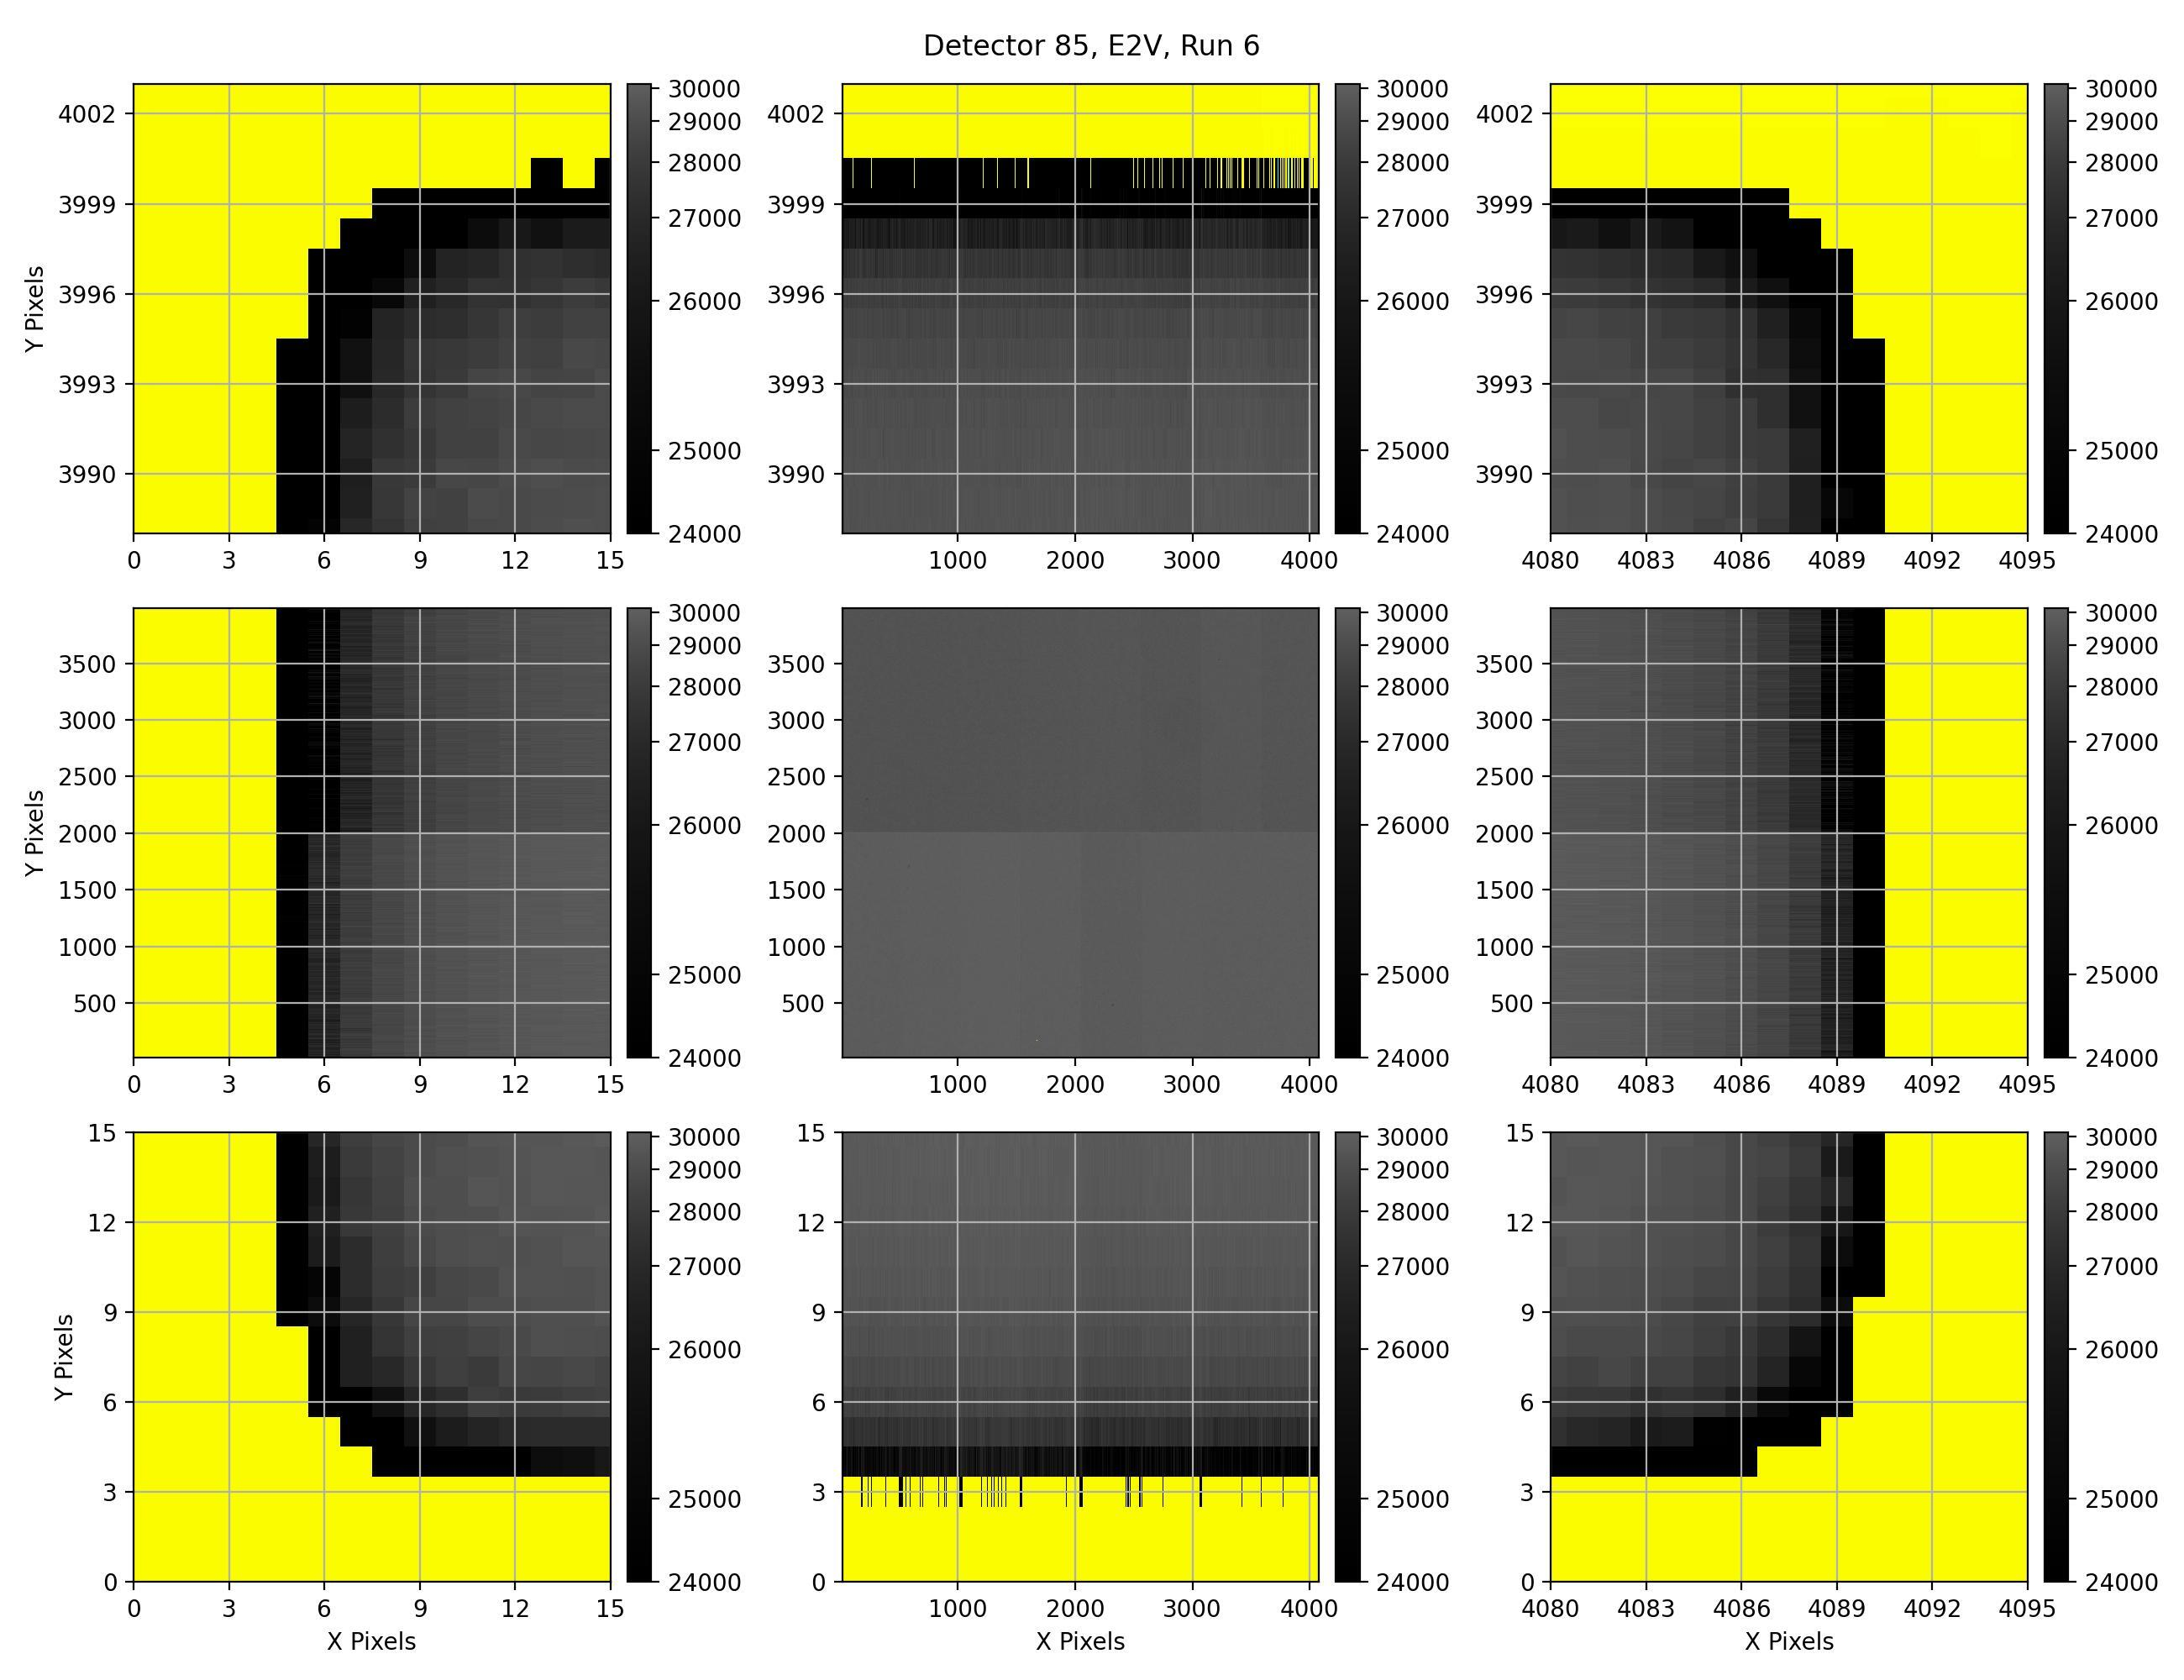
\includegraphics[width=0.9\textwidth]{sections/figures/baselineCharacterization/detector_85.jpg}
\end{centering}
\end{figure}

Due to the contamination of the edge frame response, it is difficult to
extract useful information about the dark defects in the focal plane.
The configuration for generating dark defects considers a border pixel
region that is masked differently from the dark pixels. The default
configuration has a border of zero. The largest region allowed for the
picture frame region is 9 pixels, determined by LCA-19363. Due to
incompatibility with the current pipelines, a direct comparison of a 9
pixel mask using run 6 data is not currently available. However, a 9
pixel mask can be applied to the Run 7 data.

Add conclusion when pipelines on E1071 are complete

\subsubsection{Persistence}\label{persistence}

Persistence is a feature in LSSTCam where charge is trapped in the
surface layer after high flux exposures
\hyperref[persistence-2]{{[}Persistence{]}}. Persistence is described in
detail in the
\href{https://sitcomtn-148.lsst.io/\#persistence-optimization}{persistence
optimization section}. Here we will consider the measurements taken as
part of a persistence measurement task in the typical B protocol. For a
persistence measurement, a high flux acquisition is taken, followed by a
sequence of dark images. The persistence signal has been shown to
decrease in subsequent dark images. To create a metric for persistence,
one can take the difference between the residual ADU in the first dark
image and the average of the residual ADU in the final dark images.

\begin{figure}
\begin{centering}
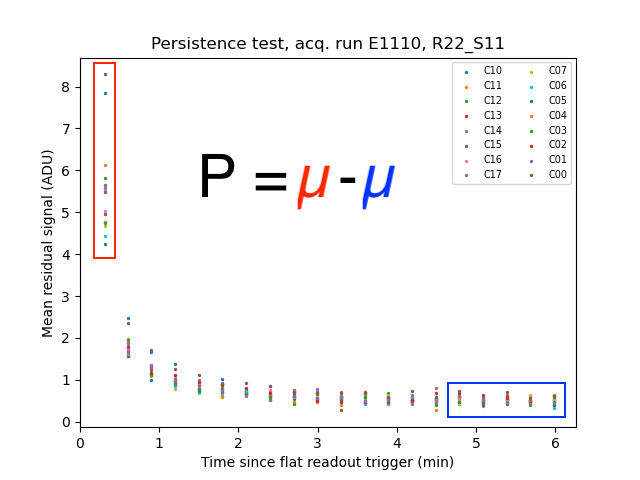
\includegraphics[width=0.9\textwidth]{sections/figures/baselineCharacterization/persistence_plot_LSSTCam_R22_S11_u_lsstccs_eo_persistence_E1110_w_2024_35_20240926T235141Z.png}
\end{centering}
\end{figure}

In the initial run 7 measurements, we have not changed any operating
parameters of LSSTCam, so we would expect persistence to still be
present in the focal plane.

\begin{figure}
\begin{centering}
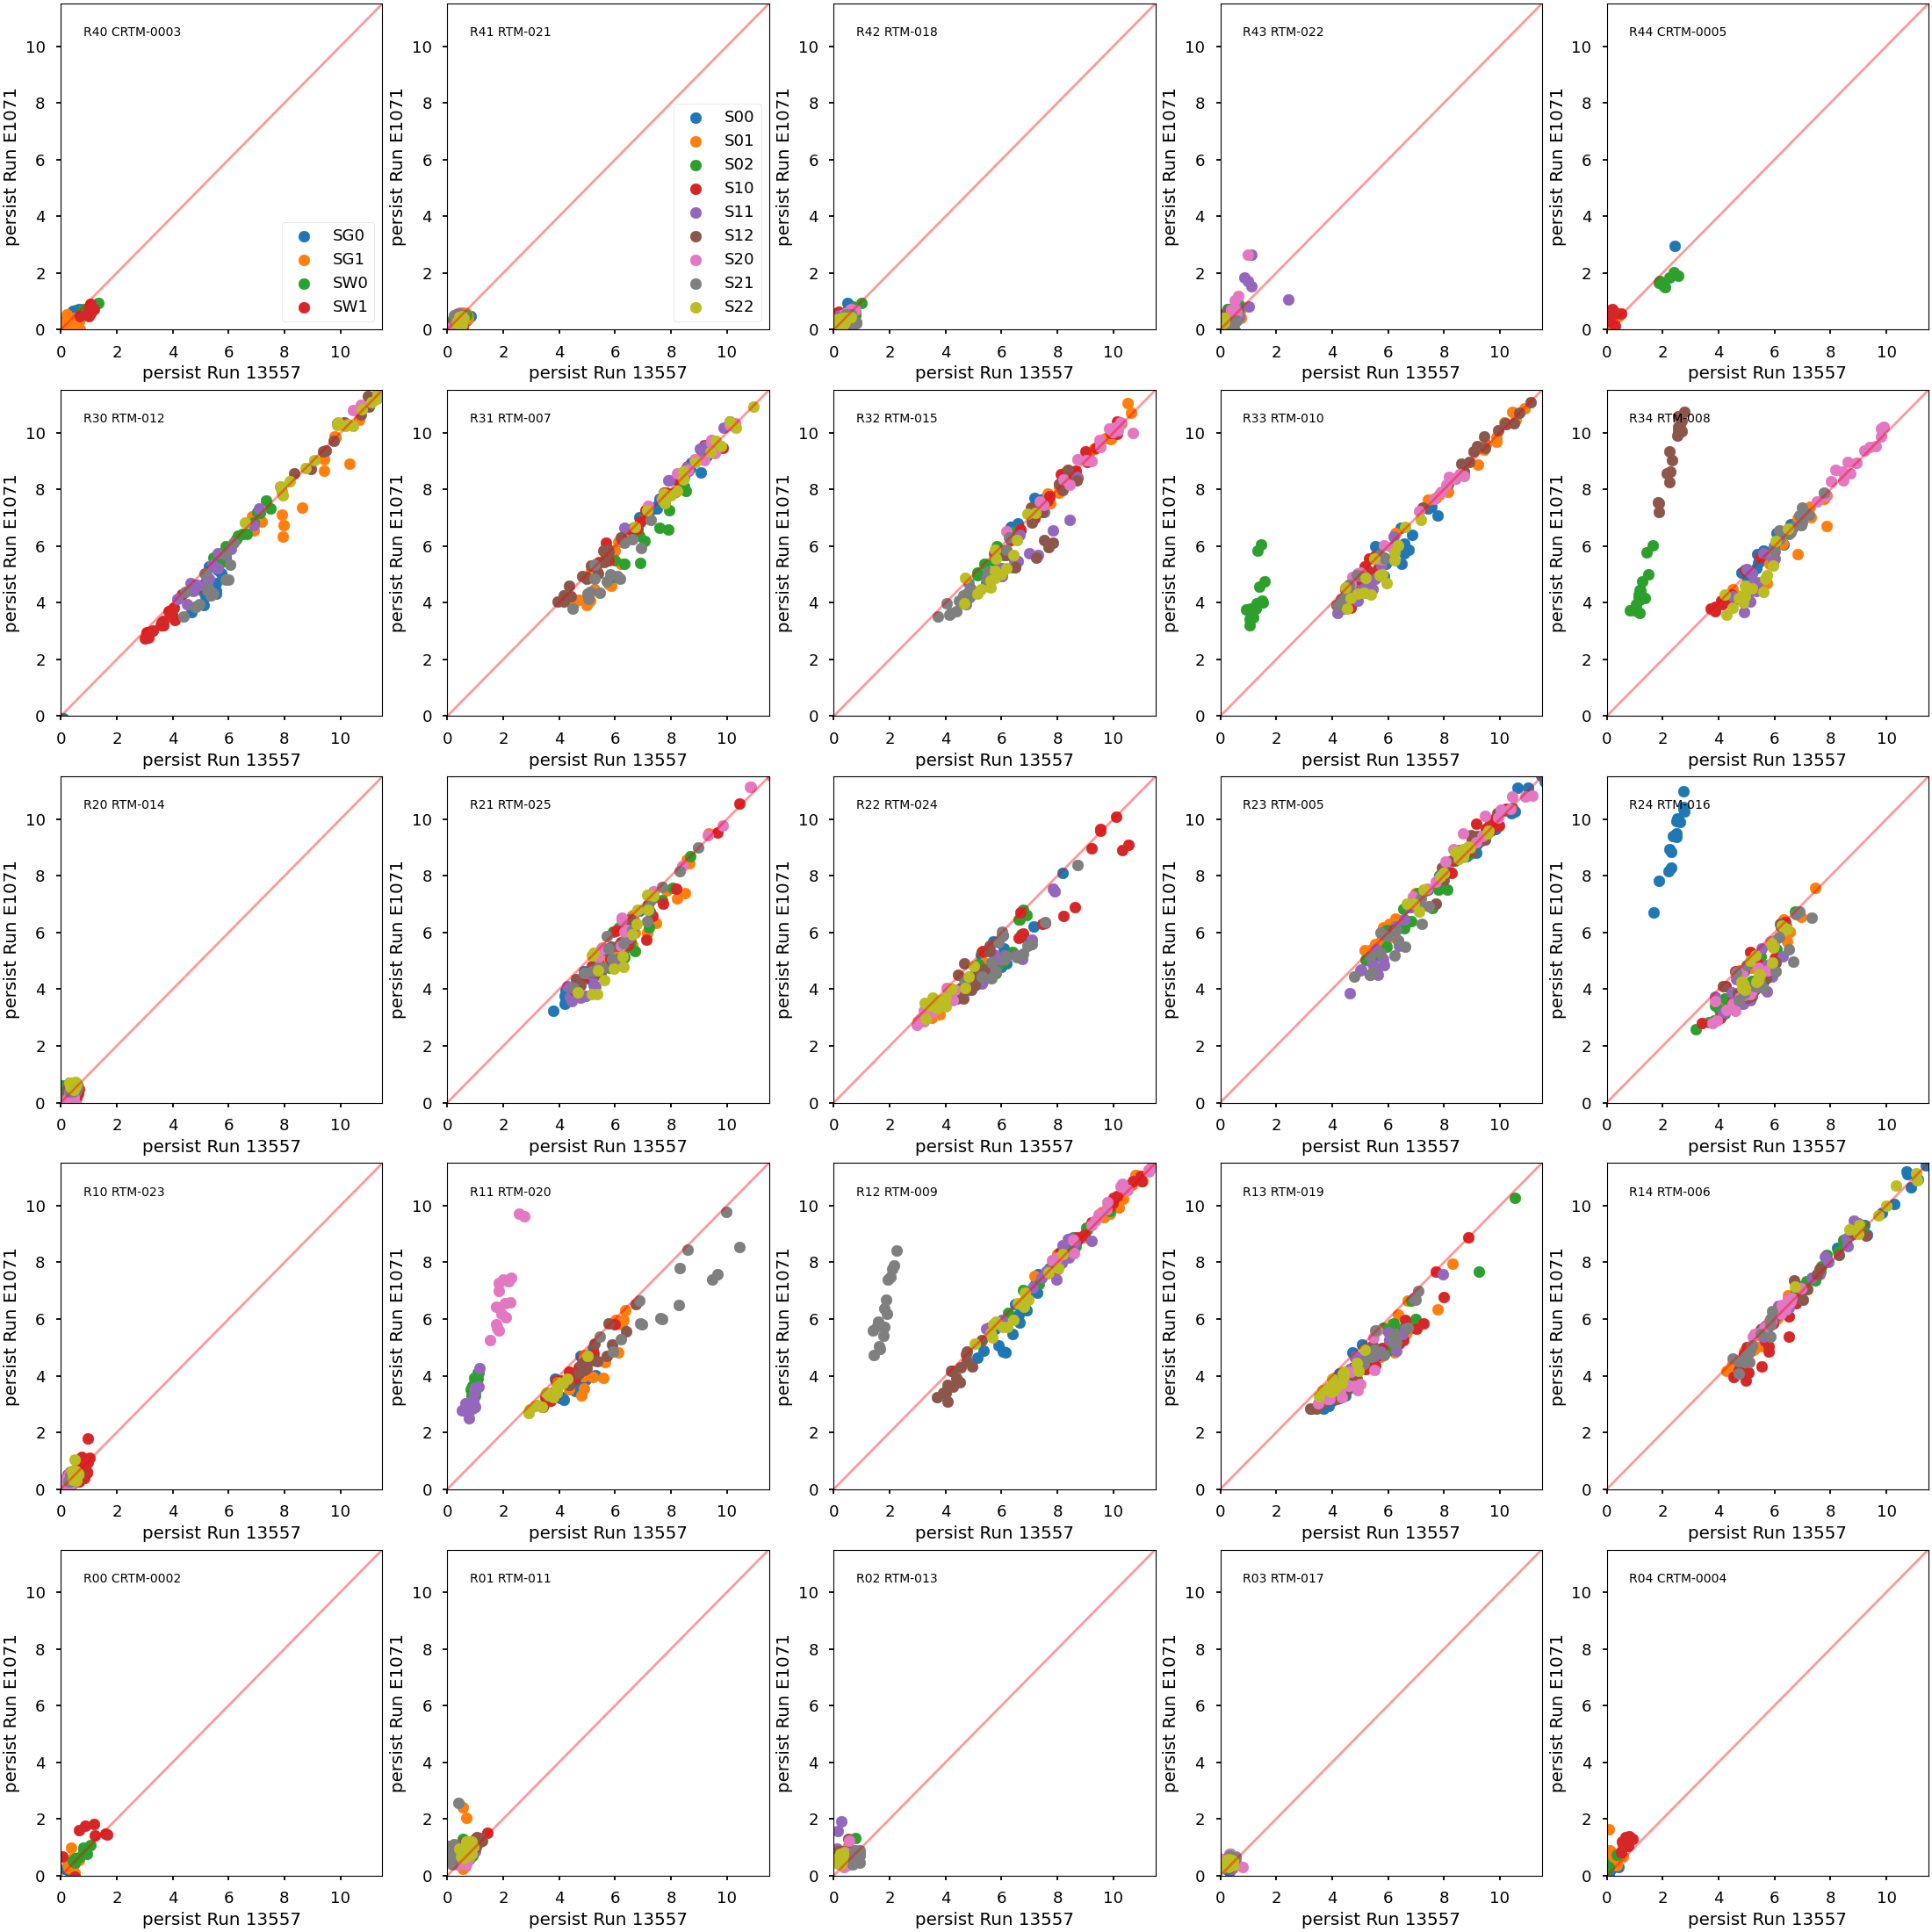
\includegraphics[width=0.9\textwidth]{sections/figures/baselineCharacterization/13557_E1071_persist.png}
\end{centering}
\end{figure}

Both runs show a consistent persistence signal in E2V sensors. Several
outliers exist with higher persistence signal in Run 7. The outliers in
these measurements are due to higher initial persistence signal
measurements, resulting in an excess of \textasciitilde5 ADU when
comparing run 6 with run 7.

\begin{figure}
\begin{centering}
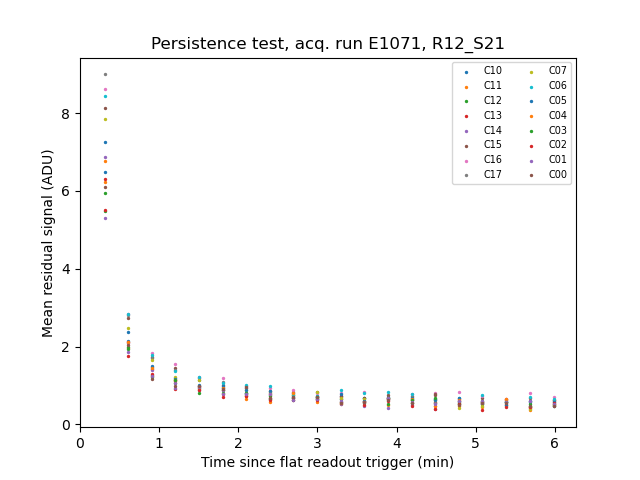
\includegraphics[width=0.9\textwidth]{sections/figures/baselineCharacterization/persistence_plot_LSSTCam_R12_S21_u_lsstccs_eo_persistence_E1071_w_2024_35_20240925T180602Z.png}
\end{centering}
\end{figure}

\begin{figure}
\begin{centering}
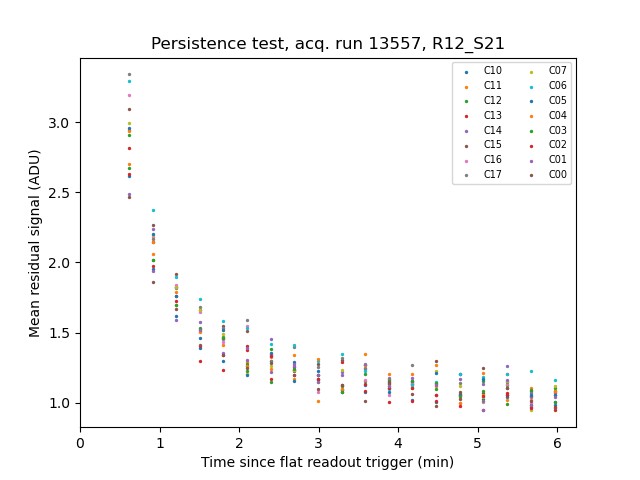
\includegraphics[width=0.9\textwidth]{sections/figures/baselineCharacterization/persistence_plot_LSSTCam_R12_S21_u_lsstccs_eo_persistence_13557_w_2023_41_20231118T050437Z.png}
\end{centering}
\end{figure}

\subsubsection{Differences from previous runs}\label{differences-from-previous-runs}

I will add this once we have agreed upon the set of parameters important
for characterization


\section{Camera Optimization}\label{camera-optimization}

\subsection{Persistence optimization}\label{persistence-optimization}

Leftover signal in the following dark after a blast of illumination has
been observed. It is called "Persistence". Persistence has been observed
in an early prototype E2V sensor as early as 2014
(\hyperref[D2014]{{[}D2014{]}}). It was confirmed that the amplitude of
the persistence decreased as the parallel swing voltage got smaller.
This is consistent with the Residual Surface Image
\hyperref[J2001]{{[}J2001{]}} -\/- the excessive charges are being stuck
at the surface layer. The level of persistence is about 10-\/-20 ADU,
and the decaying time constant is about 30 sec
\hyperref[dmtn-276]{{[}dmtn-276{]}}.

During the EO testing in 2021, we also found the persistence made a
streak toward the readout direction from the place where the bright spot
located in a previous image. We call this trailing persistence.

E2V sensors have another major problem, so-called "tearing", which is
considered a consequence of the non-uniform distribution of holes. Our
primary focus in the optimization was given to mitigate the tearing over
years, and we have successfully eliminated the tearing by bringing the
E2V voltage from the unipolar voltage (both parallel rails high and low
are positive) to the bipolar voltage (the parallel high is positive, and
the low is negative) following the formula
\hyperref[Bipolar]{{[}Bipolar{]}}. However, the persistence issue still
remained unchanged.

For the persistence issue, if this is the residual surface image, two
approaches could be taken as discussed in \hyperref[U2024]{{[}U2024{]}}.
Either 1) establishing the pinning condition where the holes make a thin
layer at the front surface so that the excessive charges recombine with
the holes or 2) narrowing the parallel swing so that the accumulated
charges in the silicon do not get close to the surface state.

The pinning condition could be established by bringing the parallel low
voltage down as low as -7V or lower. The transition voltage needs to be
empirically determined. However, E2V pointed out that the measured
current flow increases as the parallel low voltage goes low, which
increases the risk of damaging the sensor by making a
breakdown\footnote{We note that ITL operates at the parallel low voltage
  of -8V. We have observed the increased current flow. But we have the
  software protection so that the current flow does not go too high.}.
Also, the excessive charges could get recombined by the thin layer of
the holes, which could disturb the linearity at the high flux end where
charges start to interact with the holes.

The parallel swing determines the fullwell. Depending on whether the
accumulated charges spread over the columns or interact with the surface
layer, there are blooming fullwell regimes and the surface fullwell
regime. The fullwell between these two regimes is considered as the
optimal fullwell \hyperref[J2001]{{[}J2001{]}}, where we
don\textquotesingle t have persistence and as high dynamic range as
possible. Seeing the persistence, we likely operate the sensor in the
surface fullwell condition and we need to go to a narrower voltage to
get the blooming fullwell or the optimal fullwell. The obvious downside
is to narrow the fullwell.

The voltages are defined relative to each other. Changing the parallel
swing (for example) also requires changes to all other voltages to
operate the sensor properly, for example, properly reset the amplifier.
The initial voltage was given in the original formula
\hyperref[Bipolar]{{[}Bipolar{]}} but to go to the narrow voltage we had
to switch to the new formula in order to satisfy constraints
\hyperref[PersistenceMitigationVoltage]{{[}PersistenceMitigationVoltage{]}}.

\hyperref[S2024]{{[}S2024{]}}, set up a single sensor test-stand at UC
Davis. They attempted multiple different approaches mentioned above and
reported the results \hyperref[DavisReport]{{[}DavisReport{]}}. The
summary is as follows:

\begin{itemize}
\tightlist
\item
  The new voltages following the rule work fine.
\item
  Narrowing the parallel swing eliminates the persistence.
\item
  Lowering the parallel low voltage didn\textquotesingle t seem to work
  as we expected; the going further negative voltage is probably needed.
\end{itemize}

Note that the UCD setup didn\textquotesingle t show up the persistence.
It might be due to the characteristic of the sensor, or might be due to
the difference in the electronics (the long cable between CCD and REB,
for example). They need to move the parallel rails up.

\subsubsection{Persistence
optimization}\label{persistence-optimization-1}

Based on this test result, we decided to try out the new voltage with
the narrower voltage swing on the main camera focal plane. Keeping the
parallel low voltage at -6V in order to operate the sensor safely (very
conservative limit), we changed the parallel swing voltage from 9.3V to
8.0V as well as all the other voltages using the new formula. We
overexposed CCDs and took 20 darks after. The image shown below is the
mean or median of pixel-by-pixel difference between the first and the
last dark exposures, as a function of the parallel swing. As the
parallel swing is lowered, the residual signal becomes small; it becomes
roughly 10 times lower than the original 9.3V. Although we sampled
midpoints between 8.0 and 9.3V, 8.0V appears to work the best and could
be lower with the penalty of losing the full well.

\begin{figure}
\begin{centering}
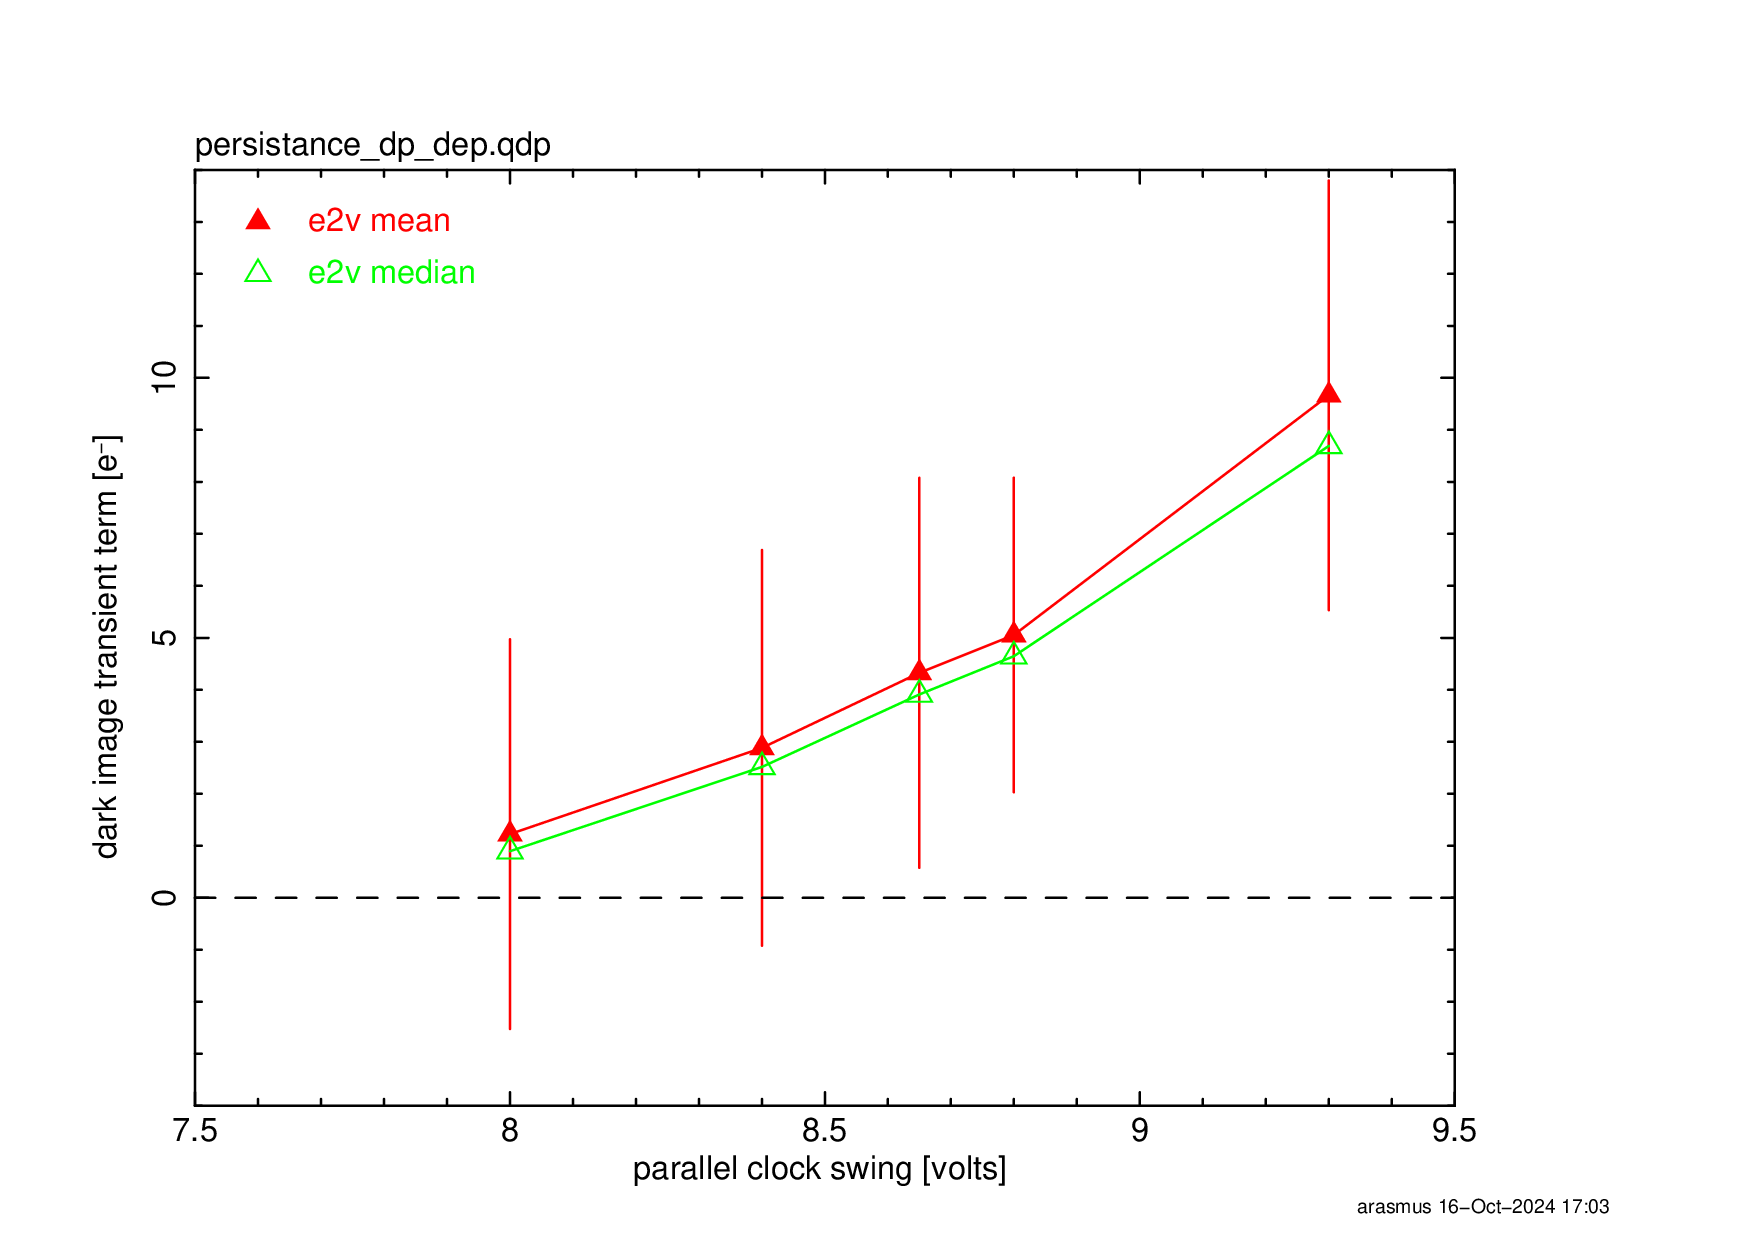
\includegraphics[width=0.9\textwidth]{sections/figures/e2v_transient_dark_vs_dp.png}
\end{centering}
\caption{The remaining charges measured in every amplifier but
aggregated by mean or median as a function of the parallel clock swing
are shown.}
\end{figure}

The following figures display how the persistence is reduced by the
voltage change. The images were processed by the standard instrumental
signature removal and get assembled in the full focal-plane view. The
dark exposure was taken right after the 400ke-equivalent flat exposure.
The figure shows the distinct pattern of elevated signal associated with
the vendor. The inner part of the focal plane is filled by e2v sensors
which have the persistence signal.

\begin{figure}
\begin{centering}
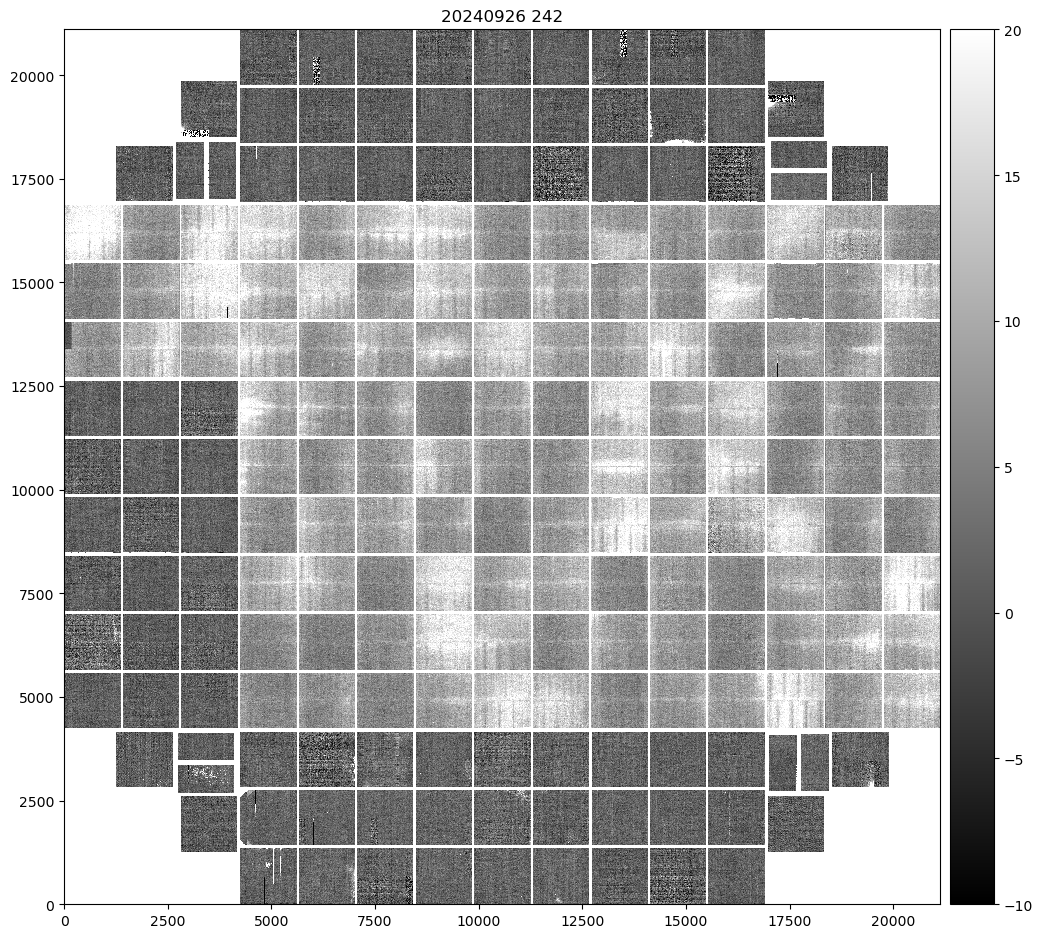
\includegraphics[width=0.9\textwidth]{sections/figures/E1110dp93.png}
\end{centering}
\caption{The first dark exposure after a 400k flat image under the
parallel swing of 9.3V (Run E1110).}
\end{figure}

The next figure shows the same dark exposure but taken with the narrow
parallel swing voltage of 8.0V. The distinct pattern goes away. This
demonstrates the persistence in e2v sensors becomes the level of
ITL\textquotesingle s ones.

\begin{figure}
\begin{centering}
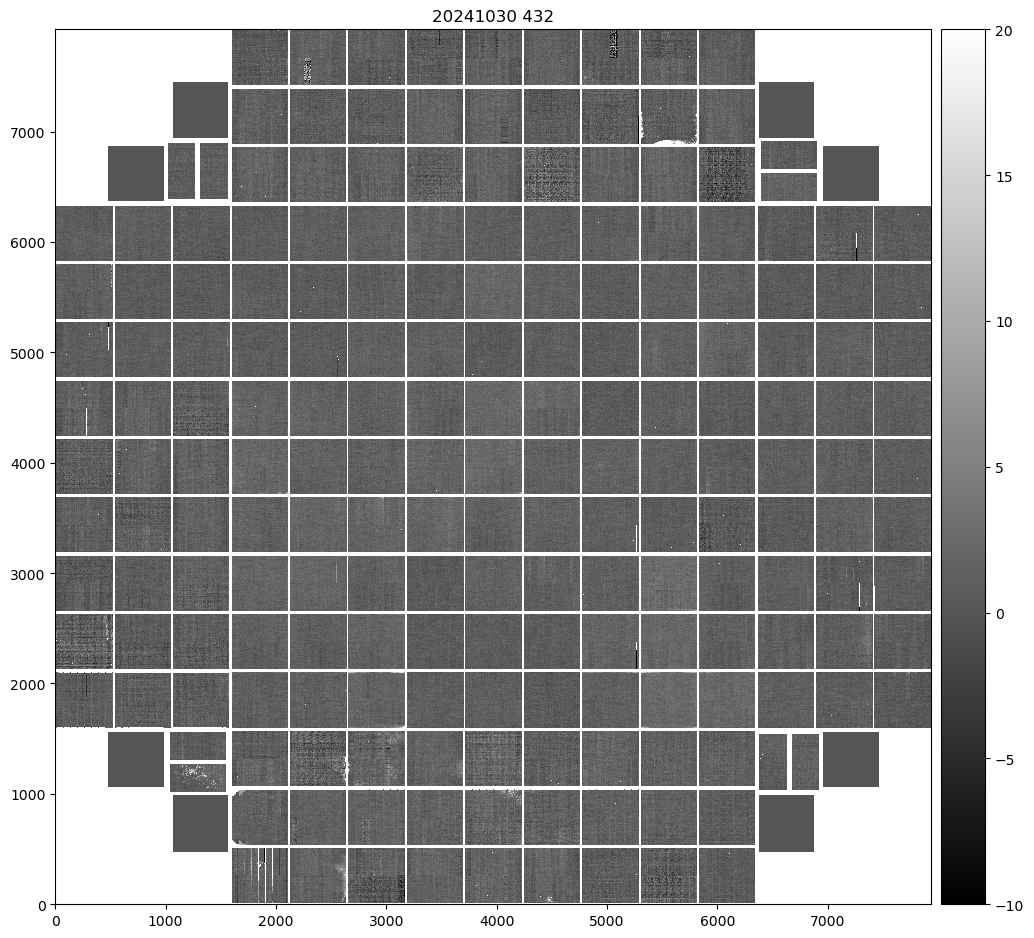
\includegraphics[width=0.9\textwidth]{sections/figures/E1880dp80.png}
\end{centering}
\caption{The first dark exposure after a 400k flat image under the
parallel swing of 8.0V (Run E1880). The figure shows no distinct
patterns from persistence in e2v sensors anymore. Note that the guider
sensors were not displayed here because they were in the guider mode.
Also some of residuals in ITL caused by defects disappeared because of
the employment of the new sequencer file (v30).}
\end{figure}

\subsubsection{Impact on full-well}\label{impact-on-full-well}

Reduction of the full well is expected by narrowing the parallel swing
voltage. This subsection explores how much reduction in the PTC turnoff
is observed in the dense PTC run. Two runs are acquired with identical
setting except for the CCD operating voltage (E1113 for 9.3V and E1335
for 8.0V). As the PTC turnoff is defined in ADU, it needs to be
multiplied by PTC\phantomsection\label{gain}{GAIN} to make a comparison.
The figure below compares the PTC turnoff in electrons and their
difference in ratio. The median reduction was 22\% .

\begin{figure}
\begin{centering}
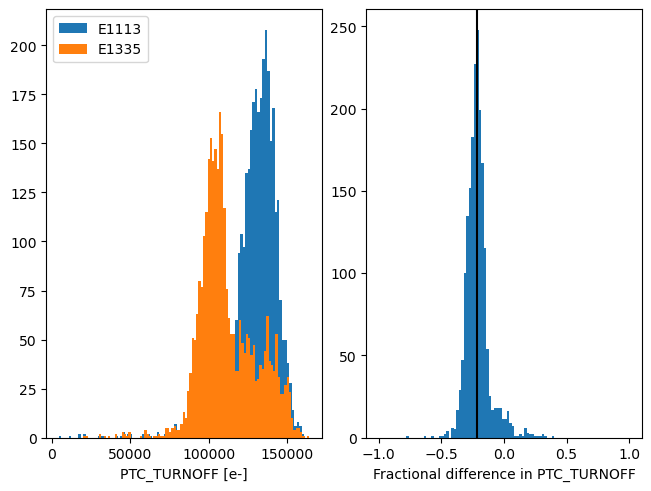
\includegraphics[width=0.9\textwidth]{sections/figures/PtcTurnoffRatio.png}
\end{centering}
\caption{Histograms of the PTC turn offs (left) and the ratios of
differences (right) between E1113 (9.3V) vs E1335 (8.0V). The median of
the reduction is 22\%.}
\end{figure}

\subsubsection{Impact on Brighter-Fatter
effect}\label{impact-on-brighter-fatter-effect}

Reducing the parallel swing is expected to enhance the brighter-fatter
effect (BFE), possibly in an anisotropic way. The BFE can be
characterized via the evolution of the variance and covariances of
flatfield exposures as a function of flux. In order to evaluate the
impact of reducing the parallel voltage swing on e2v sensors, we
acquired two series of flatfield exposures with the respective voltage
setups and extracted the "area" coefficients the "area" coefficients
(Equation (1) in \hyperref[A2023]{{[}A2023{]}}) from these two data
sets. The area coefficients describe by how much a unit charge stored in
a pixel wil alter the area of some other pixel (or itself). We find that
reducing the parallele swing from 9.3V to 8V typically increases the
area coefficients by 10\% (between 5 and 19\% depending on distance),
and the increase is almost isotropic (along serial and parallel
directions). From these measurements, we anticipate that the increase of
star sizes with flux will not become more isotropic at 8V than it was at
9.3V, and hence does not introduce new threats on the measurement of the
PSF ellipticity

\begin{figure}
\begin{centering}
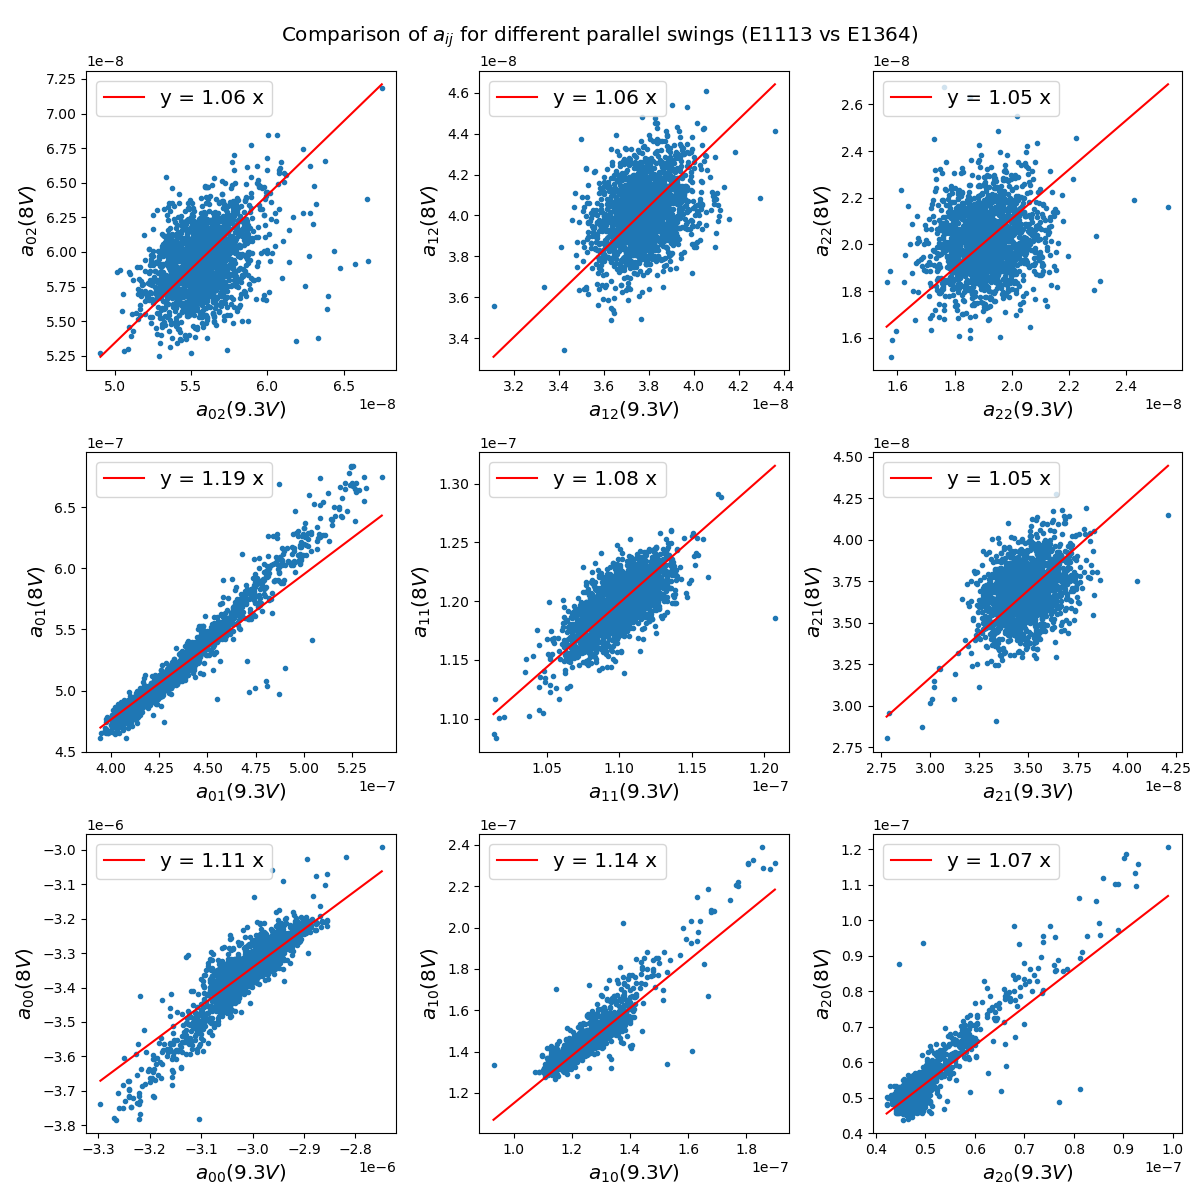
\includegraphics[width=0.8\textwidth]{sections/figures/aScatterPlots8vs9-3.png}
\end{centering}
\caption{Scatter plots of area coefficients (one entry per amplifier)
measured at 8V and 9.3V. The 9 subfigures correspond to separations
between the source of the area distortion and its victim, with the self
interaction at the bottom left. The first neighbors increase
respectively by 19\% in the parallel direction by 14\% in the serial
direction. So the BFE is slightly larger at 8V but not significantly
more anistropic.}
\end{figure}


\subsection{Sequencer Optimization}\label{sequencer-optimization}



Several efforts were undertaken to improve the sequencer files during this Run. The following points summarize the key investigations:

\begin{itemize}
\item Clears:  The complete discussion is provided in
  \href{https://sitcomtn-148.lsst.io/\#serialRemnants}{Improvement of
  Clear CCD}, but here is a summary:

  \begin{itemize}
  \item
    \textbf{No Pocket}
  We introduced the V29\phantomsection\label{nop}{NoP} (No Pocket)
  sequencer, which is an improved clear method using a serial register
  configuration that reduces the formation of pockets at the Image/Serial
  register interface. This clear method showed an approximately 2x
  improvement in the saturated image clear for e2v devices and completely
  resolved the issue for ITL devices, except for R01\phantomsection\label{s11}{S11},
  where the No Pocket method performs approximately 2x worse than the default clear. 
  For an unknown reason, this ITL CCD exhibits a significant amount of uncleared charges 
  (hundreds of lines) after a saturated flat. This issue prevents the use of the No
  Pocket configuration with ITL devices.

  \item
    \textbf{No Pocket with Serial Flush}
  We introduced V29\phantomsection\label{nopsf}{NoPSF} (No Pocket with Serial Flush), an enhanced version of the No Pocket Clear
  sequencer, which includes a variable configuration of the Serial register
  during the clear process (mimicking a serial flush), to further prevent the
  formation of pockets. This solution has been shown to completely prevent the presence of leftover charges after clearing a saturated image for e2v devices.
  \end{itemize}
  

\item Phase overlap during parallel transfer for e2v: e2v sensors feature four parallel phases. To improve the uniformity of the full well across a sensor, overlapping two phases during each time slice of the parallel transfer was introduced. However, this overlap is known to cause trailing persistence, as reported in \ref{DavisReport}. We conducted several runs using both intermediate overlapping and non-overlapping sequencers. By optimizing the operating voltages to avoid charge trapping, the trailing persistence is no longer to be a concern.
\end{itemize}

\subsection{Improved Clear}\label{improved-clear}

\subsubsection{Overview}\label{overview}

In this section, we will describe the work done during Run 7 to improve
the image clear prior to collecting a new exposure.

The problem we wanted to address is the presence of residual charges in
the first lines read for an image taken just after the clear of a saturated
image. These "hard to clear" charges are associated with highly
saturated flat or column(s) (or stars as observed in AuxTel or ComCam),
which leave signal in the first lines of the following exposure. We have
the following signature of the effect:

\begin{itemize}
\item
  in all ITL CCD (except in R01\phantomsection\label{s10}{S10} for which
  the effect is much more significant and that will be addressed later
  in this section):

  \begin{quote}
  the first CCD line of an exposure read after an image with saturated
  overscan, is close to saturation and in most of the case there is also
  a small left over signal in the 2nd line read.
  \end{quote}
\item
  in e2v CCD:

  \begin{quote}
  the effect is slightly amplifier dependent, still, like in ITL, the
  first line read in an exposure following an exposure with saturated
  overscan, is close to saturation, and a significant signal is visible
  in the following 20-50 lines. (
  \texttt{see\ left\ plots\ of\ clear\ e2v\ image\textless{}fig-image-e2vclear\textgreater{}})
  \end{quote}
\end{itemize}

These leftover electrons are not associated to what we usually call 
residual image or persistence. They are suspected to be associated to
pockets, induced by the electric field configuration in the sensor and
the field associated to saturated pixels: pocket(s) that survive to a
clear, will prevent charges to be cleared. A change of the electric
field (ex: a change in clocks configuration) can remove the pockets, and
free the charges, allowing them to be cleared. If charges stuck in
pocket(s) are not removed by a clear, we observed that an image read
(ex: a bias) will fully remove them: only the first exposure taken after
an image with saturated overscan is impacted. If the clocks
configuration used in our standard clear is not able to flush away those
charges, a standard readout of \textgreater\textasciitilde{} 2000 lines
does remove them.

The localisation of these uncleared electrons in the first lines of the
CCDs, spots the interface between the image area and the serial register
as the location for those pockets. For this reason we investigated
changes in the field configuration of the serial register during the
clear, to avoid pockets at this image-serial register interface.

\subsubsection{New sequencers}\label{new-sequencers}

To addresse this clear issue, we focussed on updating the serial
register field as the lines are moved to it. The constrain being that
the changes introduced should not significantly increase the clear
execution time. It should be notice that we tried in 2021 a sequencer
called "Deep Clear" ( \hyperref[sequencerV23_DC]{{[}sequencerV23\_DC{]}}
) as a first try to address the clear issue: it added one full line
flush on top of the existing one at the end of the clear. This sequencer
did improve the clear, still not fully fixing the clear issue ( see
\texttt{Summary\ table\textless{}table-SummaryClear\textgreater{}}).

In the Run 7, We considered on top of the default clear, 2 new
configurations. The changes are in the ParallelFlush function, which
move the charges from the image area to the serial register:

\begin{itemize}
\tightlist
\item
  the default clear (V29): In the default clear, all serial clocks are
  kept up as the parallel clocks move charges from the image area to the
  serial register (\hyperref[sequencerV29]{{[}sequencerV29{]}}). The
  charges once on the serial register will hopefully flow to the ground:
  the serial register clocks being all up, without pixels boundary, and
  with its amplifier in clear state. At the end of the clear, a full
  flush of the serial register is done (\textasciitilde{} the serial
  clocks changes to read a single line ).
\item
  the No-pocket Clear (NoP): a clear where the serial register has the
  same configuration (S1 \& S2 up, S3 low) when the parallel clock P1
  moves the charges to the serial register than in a standard image read
  . Still we keept all phases up the rest of the time for a fast clear
  of the charges along the serial register
  (\hyperref[sequencerV29_NoP]{{[}sequencerV29\_NoP{]}}). The idea is
  that the S3 phase is not designed to be up when charges are transfered
  to the serail register, and is probably playing a major role in the
  pockets creation.
\item
  The No-pocket with serial flush Clear (NoPSF): this sequencer is close
  to the NoP solution , except that during the transfered of 1 line to
  the serial register, the serial phases are also moved to transfer two
  pixels along teh serial register. The changes in electric field at the
  image-serial register interface are then even more representative to
  what a standard read will produce, and should further prevent the
  creation of pockets.
  (\hyperref[sequencerV29_NoPSF]{{[}sequencerV29\_NoPSF{]}}).
\end{itemize}

\subsubsection{Results on standard e2v and itl
CCD}\label{results-on-standard-e2v-and-itl-ccd}

\begin{figure}
\begin{centering}
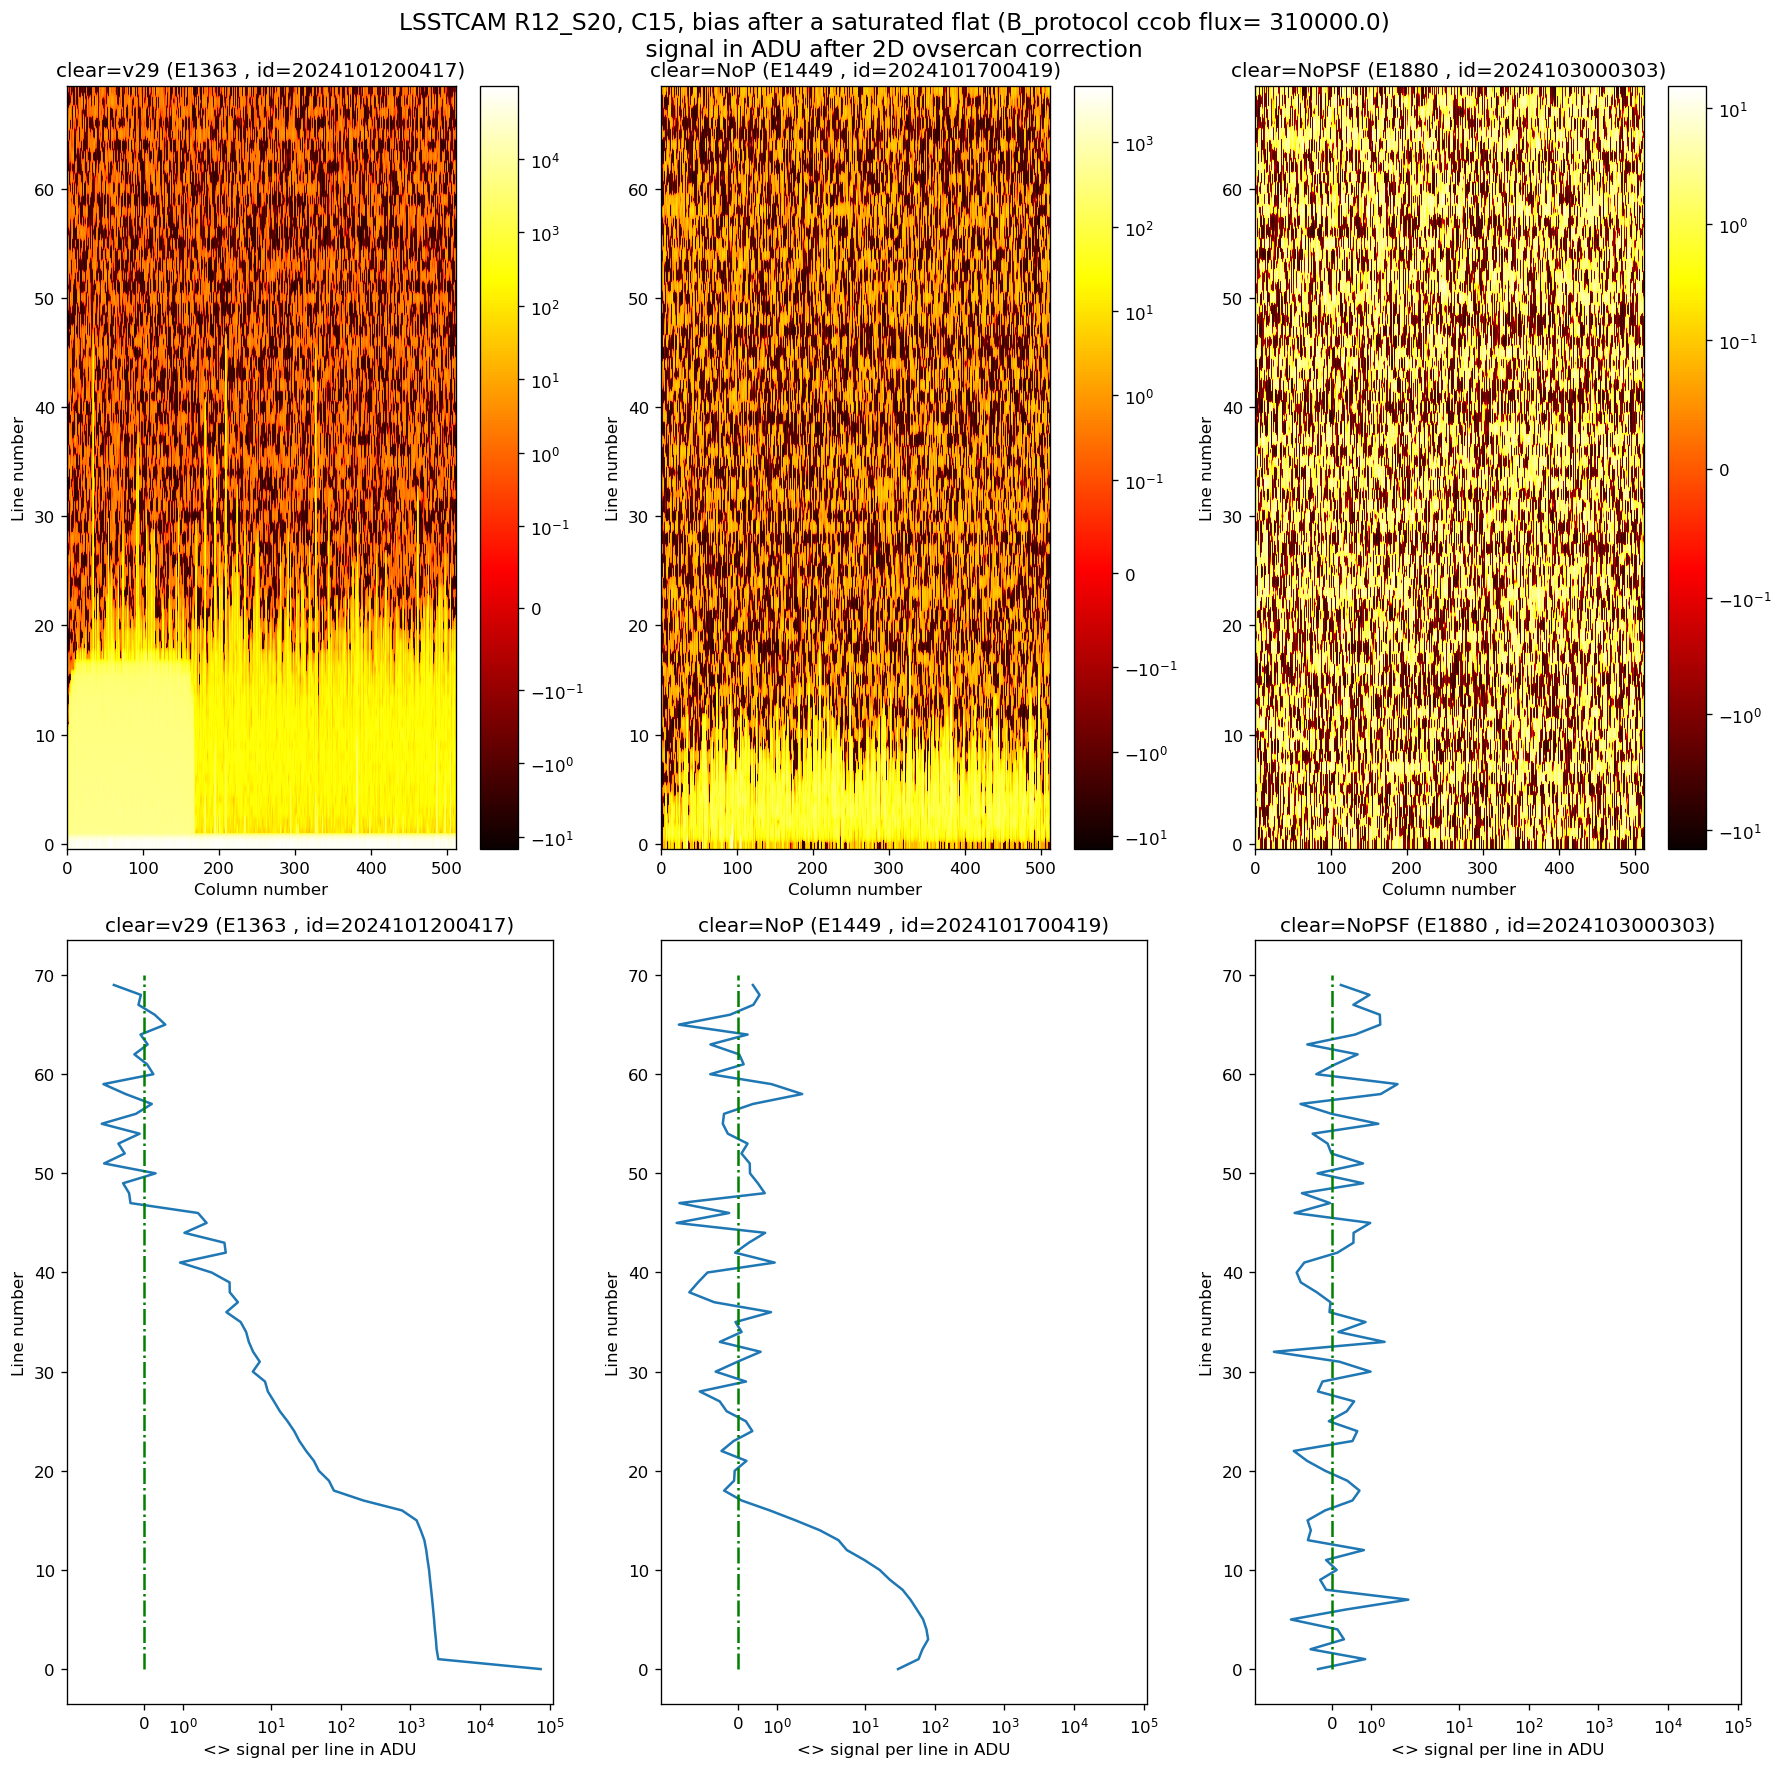
\includegraphics[width=0.9\textwidth]{sections/figures/plots_R12_S20_C15_E1880_bias_2024103000303.png}
\end{centering}
\end{figure}

\emph{Figure showing the impact of the various types of clear on a bias
taken after a saturated flat for an E2V sensor.}

\begin{figure}
\begin{centering}
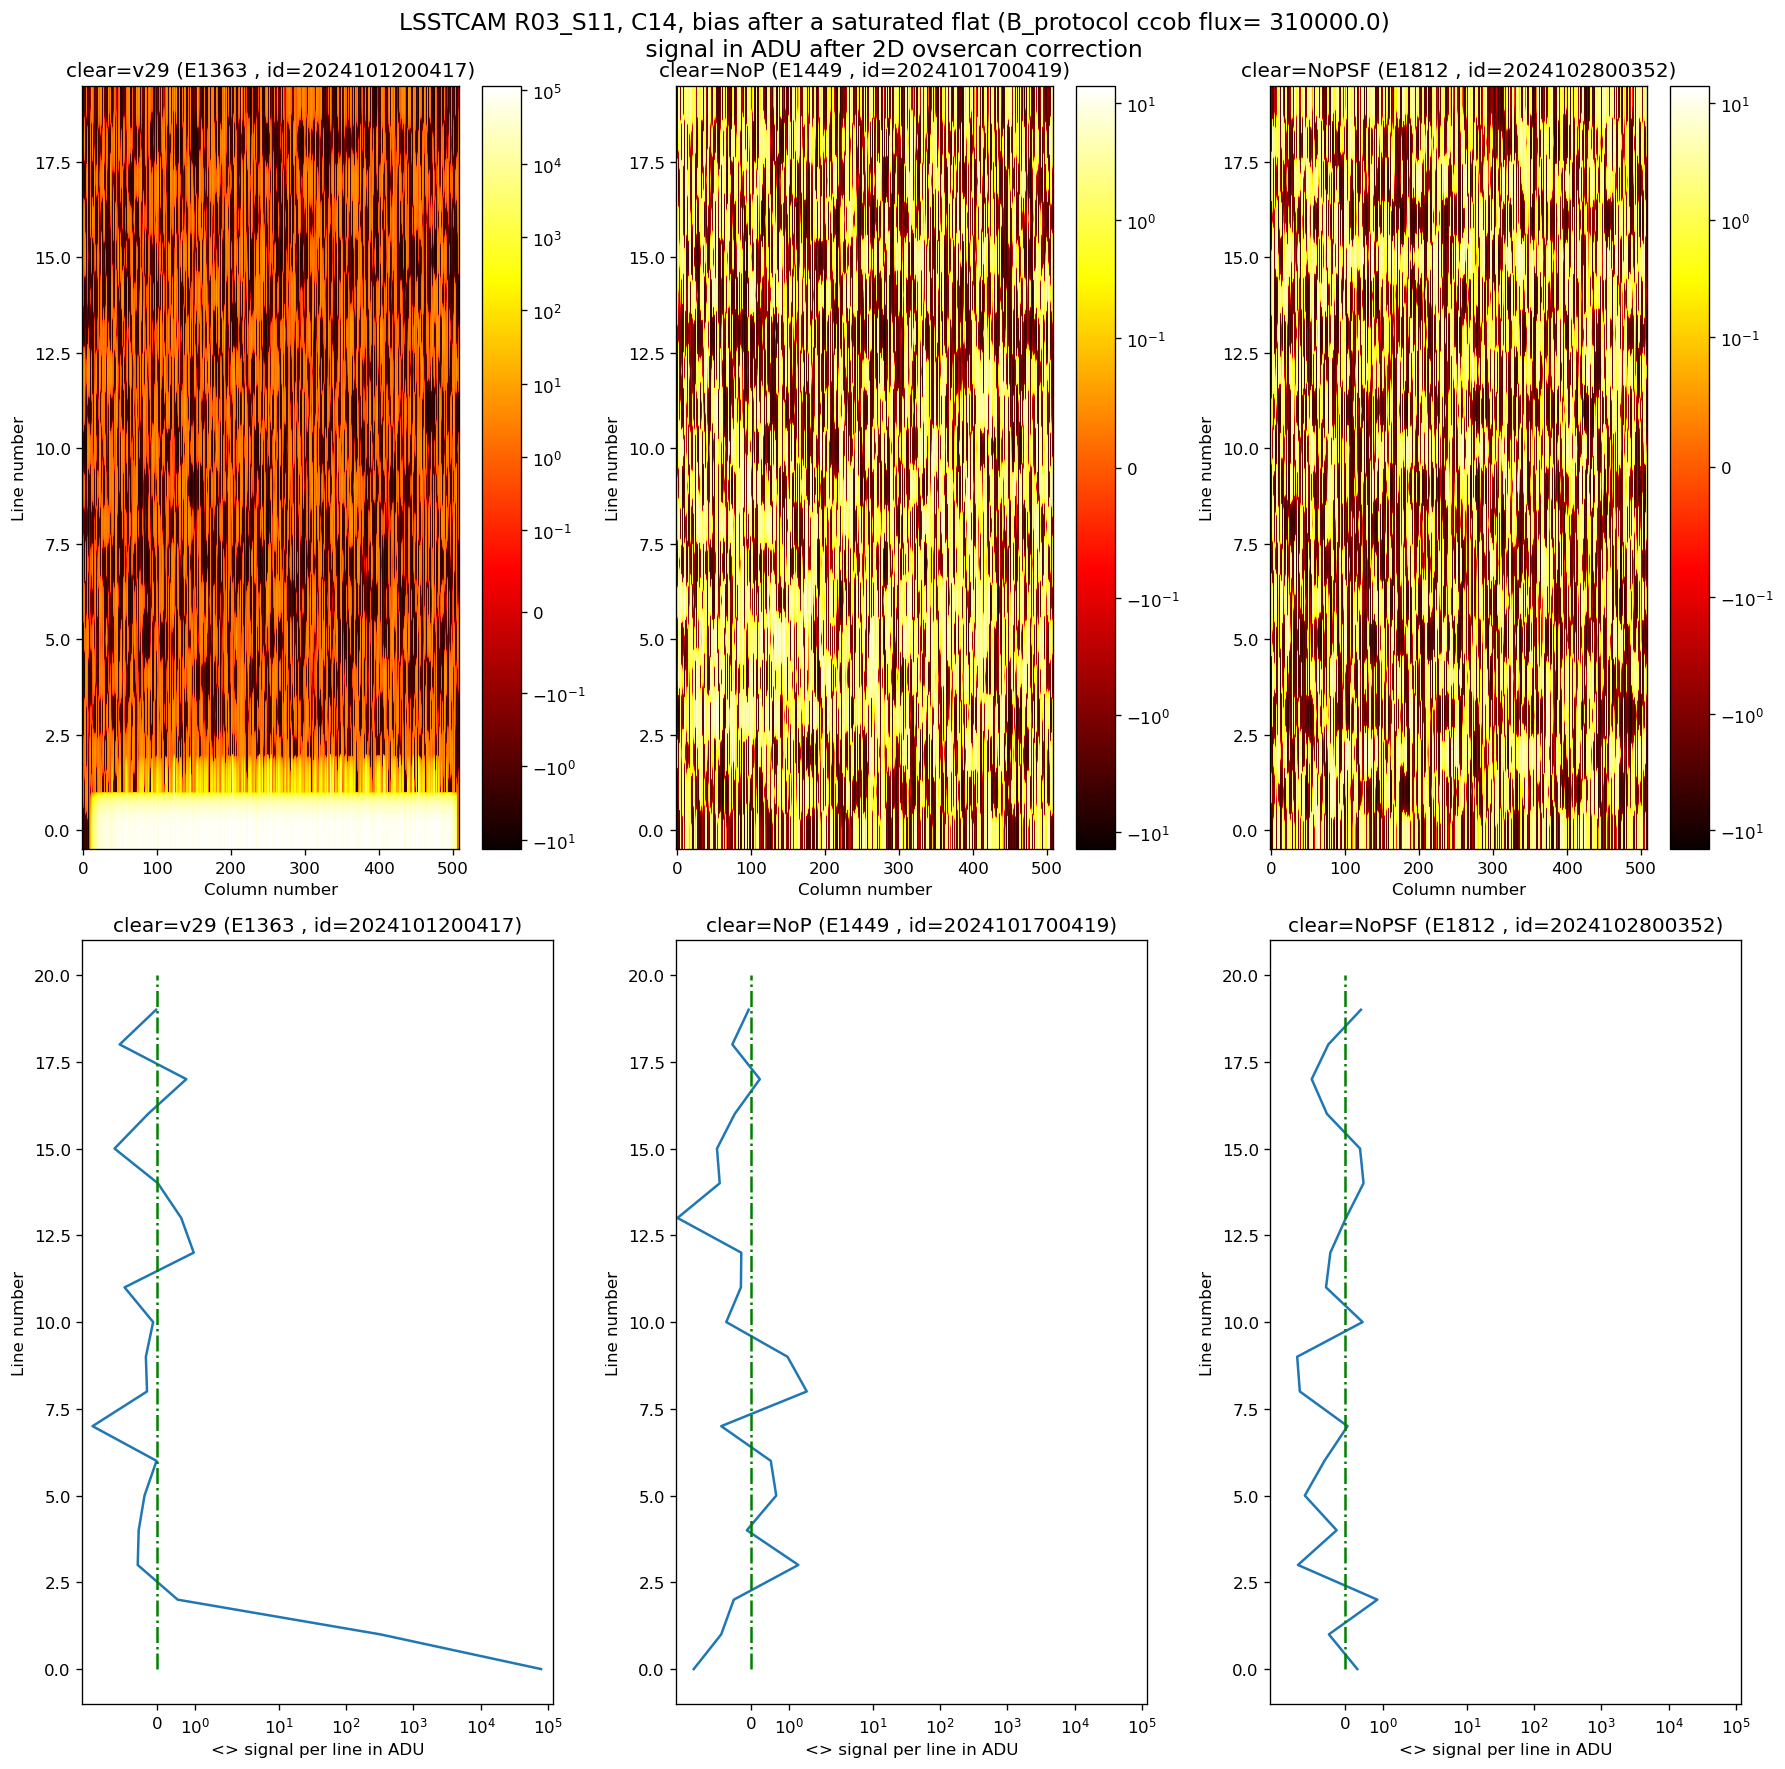
\includegraphics[width=0.9\textwidth]{sections/figures/plots_R03_S11_C14_E1812_bias_2024102800352.png}
\end{centering}
\end{figure}

\emph{Figure showing the impact of the various types of clear on a bias
taken after a saturated flat for an ITL sensor.}

In the above images, we present for 3 types of sequencer (from left to
right: V29, NoP and NopSF), a zoom on the first lines of an itl or e2v
amplifier (for itl R03\phantomsection\label{s11}{S11} C14 and for e2v
R12\phantomsection\label{s20}{S20} C10 ) shown as a 2D lines-columns
image (top plots) or as the mean signal per line for the first lines
read of an amplifier (bottom plots).

As seen in
\texttt{see\ left\ plots\ of\ clear\ e2v\ image\textless{}fig-image-e2vclear\textgreater{}}
for an e2v CCD, a bias taken just after a saturated flat will show a
residual signal in the first lines read when using the default clear
(left images,clear=v29): the first line has an almost saturated signal
(\textasciitilde{} 100 kADU here), and a significant signal is seen up
to the line \textasciitilde50. In practice, in function of the
amplifier, signal can be seen up to line 20-50. When using the NoP clear
(central plots), we can already see a strong reduction of the uncleared
charges in the first acquired bias after a saturated flat, still a small
residual signal is visible in the first \textasciitilde20 lines. The
NoPSF clear (right plots) fully clear the saturated flat, and no
uncleared charges are observed in the following bias.

As seen in
\texttt{see\ left\ plots\ of\ clear\ itl\ image\textless{}fig-image-itlclear\textgreater{}}
for an itl CCD, a bias taken just after a saturated flat will show a
residual signal in the first lines read when using the default clear
(left images,clear=v29) : the first line has an almost saturated signal
(\textasciitilde{} 100 kADU here), and a significant signal is seen in
the following line. Both NoP clear (central plots) and NoPSF clear
(right plots) fully clear the saturated flat, and no uncleared charges
are observed in the following bias.

\subsubsection[Results on itl R01]{\texorpdfstring{Results on itl
R01\protect\hypertarget{s10}{}{S10}}{Results on itl R01S10}}\label{results-on-itl-r01s10}

\begin{figure}
\begin{centering}
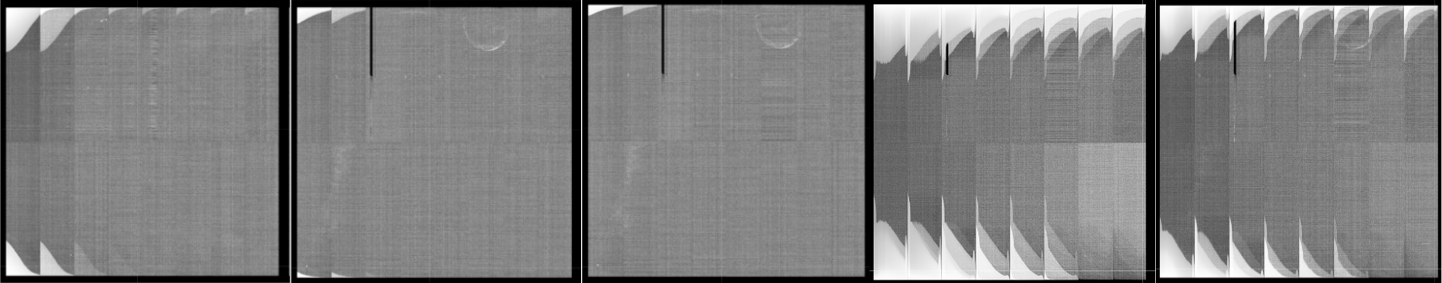
\includegraphics[width=0.9\textwidth]{sections/figures/Clear_R01_S10.png}
\end{centering}
\end{figure}

\emph{Figure showing the impact of the various types of clear on ITL
R01\_S10 after a saturated flat (bias after a saturated flat), from left
to right: 1 standard Clear, 3 standard Clear, 5 standard Clear, 1 NoP
Clear, 1 NoPSF Clear}

There is one ITL sensor, R01\phantomsection\label{s10}{S10}, that
presents a specific and non-understood behavior:

\begin{itemize}
\tightlist
\item
  It has a quite low full well (2/3 of nominal)
\item
  The 3 CCD of this REB have a gain 20\% lower than all other ITL CCD?
\item
  The images taken after a large staturation, as seen in figure
  \texttt{clear\ in\ itl\ R01\_S10\ \textless{}fig-image-itlR01\_S10clear\textgreater{}},
  show a large amount of uncleared charged (with the standard clear: 4
  amplifiers with \textasciitilde500 lines of saturated signal!)
\end{itemize}

It apears that putting S3 low during the clear as done in NoP or NoPSF,
is even worse than a standard clear. This is strange as a full frame
read, which does this too, manages to clear such image. We can notice
that NoPSF is \textasciitilde50\% better than NoP, but still worse than
the standard clear, in particular for the 12 amplifiers almost correct
with the standard clear.

At this stage we don\textquotesingle t have a correct way to clear this
sensor once it collects a saturated flat, but It\textquotesingle s not
known if a saturated star in this sensor, leaving signal in the
parallele overscan, will presents the same clear issue.

\subsubsection{Conclusion}\label{conclusion}


{\small
\begin{longtable}{|p{0.17\linewidth}|p{0.17\linewidth}|p{0.17\linewidth}|p{0.17\linewidth}|p{0.17\linewidth}|p{0.17\linewidth}|}
\caption{\emph{This table summarizes the different clear methods used so far.}} \\
\hline
\textbf{Clear Type} & \textbf{Clear duration} & \textbf{"E2V" after saturated Flat} & \textbf{"ITL" after saturated Flat} & \textbf{R01 ITL "unique"} \\
\hline
\endfirsthead

\hline
\textbf{Clear Type} & \textbf{Clear duration} & \textbf{"E2V" after saturated Flat} & \textbf{"ITL" after saturated Flat} & \textbf{R01 ITL "unique"} \\
\hline
\endhead

\hline
\endfoot

\hline
\endlastfoot

\textbf{Default Clear} 1 Clear (seq. V29) & 65.5 ms & 1st line saturated signal up to line 50 & 1st line saturated signal up to 2nd line & first 500 lines saturated for 4 amp, 13 amp with signals \\
\textbf{Multi Clear} 3 Clears (seq. V29) & 196.5 ms & No residual electrons & No residual electrons & first 150 lines saturated for 2 amp, 5 amp with signals \\
\textbf{Multi Clear} 5 Clears (seq. V29) & 327.4 ms & No residual electrons & No residual electrons & first 100 lines saturated for 2 amp, 2 amp impacted \\
\textbf{Deep Clear} 1 Clear (Seq. V23 DC) & 64.69 ms & 1st line saturated signal up to line <20 & tiny signal left in the first line & not measured \\
\textbf{No Pocket (NoP)} 1 Clear (seq. V29) & 65.8 ms & signal up to line 20 & No residual electrons & first 1000 lines saturated for 16 amp, 16 amp with signals \\
\textbf{No Pocket Serial Flush (NoPSF)} 1 Clear (seq. V29, V30) & 67 ms & No residual electrons & No residual electrons & first 750 lines saturated for 16 amp, 16 amp with signals \\
\end{longtable}
}


%\begin{longtable}{|p{0.18\linewidth}|p{0.13\linewidth}|p{0.13\linewidth}|p{0.13\linewidth}|p{0.13\linewidth}|p{0.13\linewidth}|p{0.16\linewidth}|}
%\caption{\emph{This table summarizes the different clear methods used so far.}} \\
%\hline
%\textbf{} & \textbf{Default Clear 1 Clear (seq. V29)} & \textbf{Multi Clear 3 Clears (seq. V29)} & \textbf{Multi Clear 5 Clears (seq. V29)} & \textbf{Deep Clear 1 Clear (Seq. V23 DC)} & \textbf{No Pocket (NoP) 1 Clear (seq. V29)} & \textbf{No Pocket Serial Flush (NoPSF) 1 Clear (seq. V29, V30)} \\
%\hline
%\endfirsthead
%
%\hline
%\textbf{} & \textbf{Default Clear 1 Clear (seq. V29)} & \textbf{Multi Clear 3 Clears (seq. V29)} & \textbf{Multi Clear 5 Clears (seq. V29)} & \textbf{Deep Clear 1 Clear (Seq. V23 DC)} & \textbf{No Pocket (NoP) 1 Clear (seq. V29)} & \textbf{No Pocket Serial Flush (NoPSF) 1 Clear (seq. V29, V30)} \\
%\hline
%\endhead
%
%\hline
%\endfoot
%
%\hline
%\endlastfoot
%
%Clear duration & 65.5 ms & 196.5 ms & 327.4 ms & 64.69 ms & 65.8 ms & 67 ms \\
%"E2V" after saturated Flat & 1st line saturated signal up to line 50 & No residual electrons & No residual electrons & 1st line saturated signal up to line <20 & signal up to line 20 & No residual electrons \\
%"ITL" after saturated Flat & 1st line saturated signal up to 2nd line & No residual electrons & No residual electrons & tiny signal left in the first line & No residual electrons & No residual electrons \\
%R01 ITL "unique" & first 500 lines saturated for 4 amp, 13 amp with signals & first 150 lines saturated for 2 amp, 5 amp with signals & first 100 lines saturated for 2 amp, 2 amp impacted & not measured & first 1000 lines saturated for 16 amp, 16 amp with signals & first 750 lines saturated for 16 amp, 16 amp with signals \\
%\end{longtable}


Even if NoP or NoPSF are overcoming the clear issue we had with ITL
sensors, the exception of R01\phantomsection\label{s10}{S10} prevented
the usage of those sequencers for ITL device for the Run 7. Notice that
beyond R01\phantomsection\label{s10}{S10} the numbers of line potencilly
"not cleared" are small (2 first lines) in ITL device, and they
correspond to a CCD area hard to use anyway (sensor edges with low
efficciency). So at this stage the default clear is still our default
for ITL, and further studies to overcome the problem with
R01\phantomsection\label{s10}{S10} are forseen (ex: do a continuous
serial flush during exposure at low rate, 10\^{}6 pixels flush in 15s).

\begin{quote}
On the other side, after those studies in Run 7, we now have a good way
to fully clear the e2v devices through the NopSF clear. The NoPSF clear
grants that the first 50 lines of e2v device that had un-cleared
electrons from the previous exposure, are now free of such
contamination.
\end{quote}

From now:

\begin{itemize}
\tightlist
\item
  for e2v, NoPSF will be the default clear method
\item
  for ITL, the origial clear (serial phase 3 always), slightly extended
  in time to match the NoPSF e2v clear execution time, will stay the
  default method.
\end{itemize}

\subsection{Toggling the RG Bit During Parallel Transfer}\label{noRGe2v}
This investigation comes from an analogy drawn with the ITL sequencer file. Although the vendor recommended toggling the RG bit at the end of the parallel transfer, it was unclear whether this step was truly necessary. Given the improvements observed in ITL devices, applying this approach to e2v devices also became an area of interest.

\subsection{Disable IDLE FLUSH}\label{thermal-optimization}

IDLE\_FLUSH is one of the main settings in the sequencer file that enables the sequencer output to run while in the IDLE state (the period between one exposure and the next). The specific implementation of IDLE\_FLUSH can be selected from various functions in the sequencer file. In Run 5, we chose the \texttt{ReadPixel} function, which reads out a pixel. This choice was initially made to mitigate the so-called yellow corner issue—a 2D structure of elevated signal near an amplifier corner observed in e2v's bias or dark exposures for certain amplifiers (see details in \hyperref[U2024]{{[}U2024{]}}).

However, it was reported that running IDLE\_FLUSH exacerbates the Divisidero tearing issue. Divisidero tearing appears as a signal deficiency at amplifier boundaries in e2v sensors, accompanied by increased signal in adjacent columns. Additionally, using \texttt{ReadPixel} as the IDLE\_FLUSH function has the highest thermal impact because it continuously operates the Analog-to-Digital Converter at its maximum rate. This results in a significant difference in power consumption—more than 50W—between the exposure state and the IDLE state. Consequently, the focal plane experiences a temperature variation of approximately 2\degree C between periods of image acquisition and idle periods (Figure~\ref{IdleFlushEffect}).

\begin{figure}
\begin{centering}
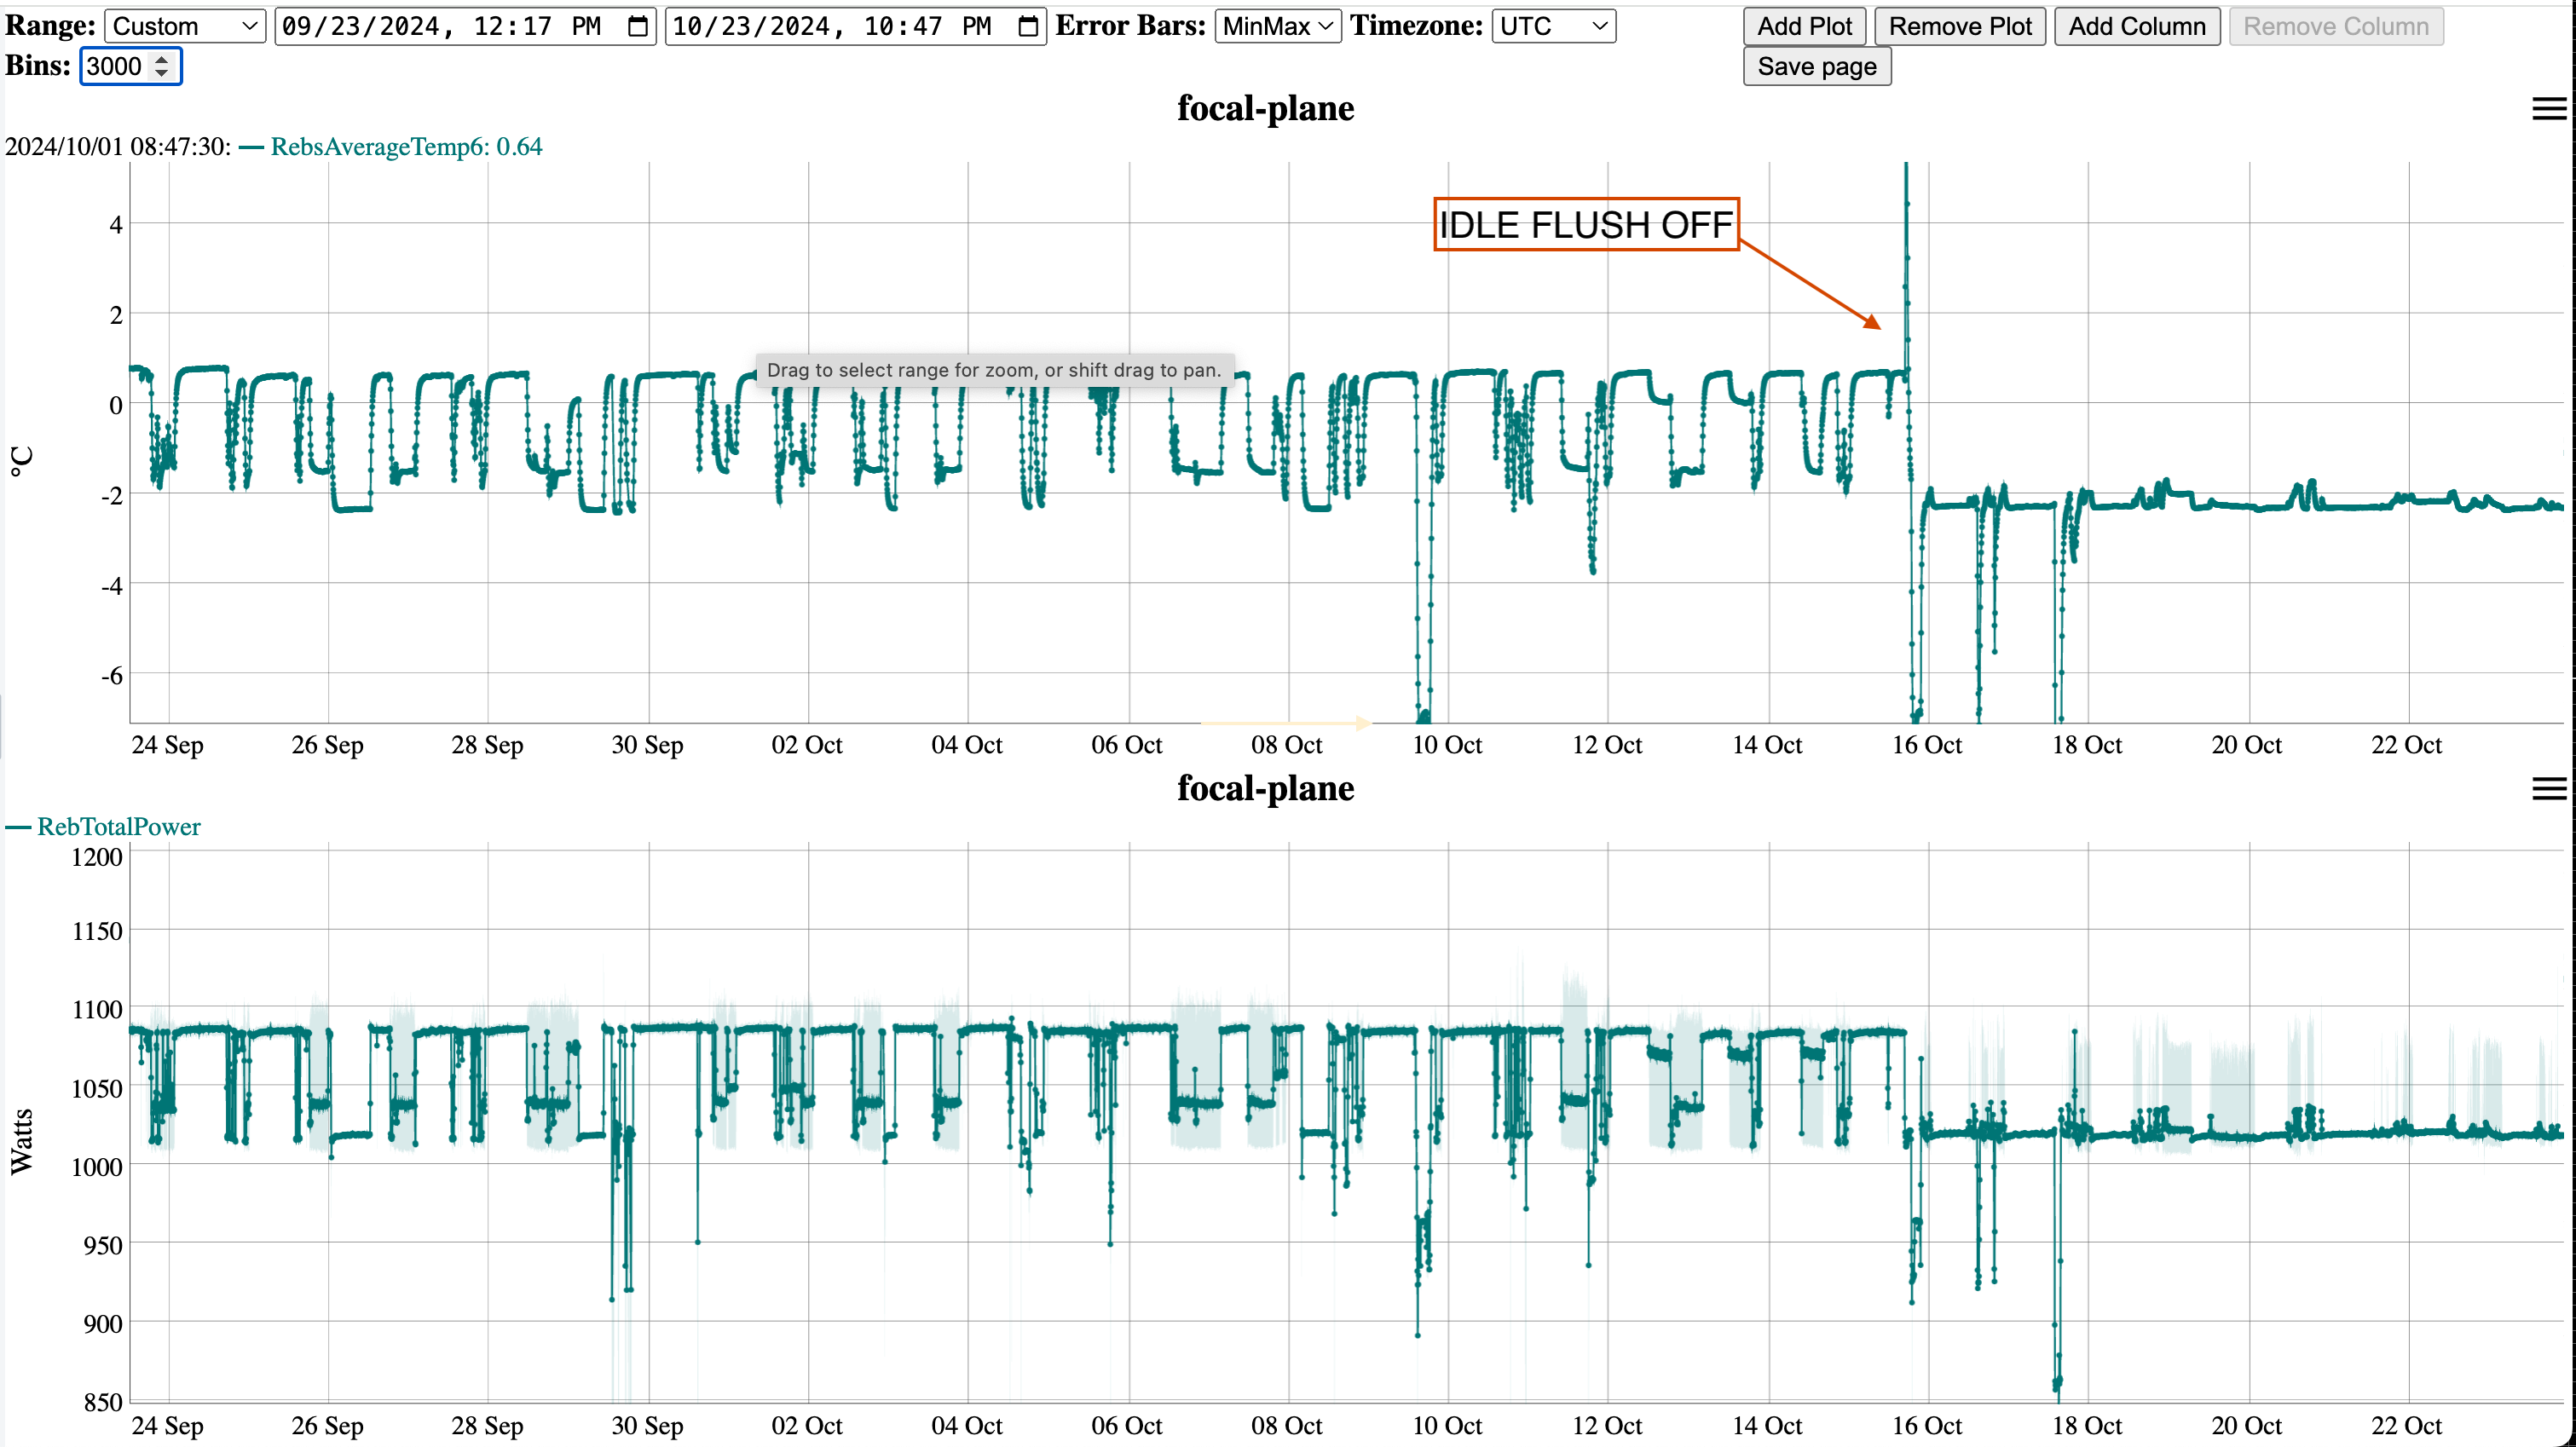
\includegraphics[width=0.8\textwidth]{sections/figures/REB_power_temp6_sept24_to_Oct23.png}
\end{centering}
\caption{Impact of enabling and disabling IDLE\_FLUSH on focal-plane temperature and power consumption.}\label{IdleFlushEffect}
\end{figure}

This temperature variation in the focal plane can lead to changes in the REB temperature, potentially causing gain variations or instability in the bias. Based on these considerations, we decided to disable IDLE\_FLUSH. The impact of this change on bias stability is discussed in Sections~\ref{bias-stability-2} and~\ref{gain-stability-2}.

\subsection{Summary}\label{summary}
E2V sensors had persistence. We confirmed changing the E2V CCD operating
voltage greatly reduced persistence. As penalties, we observed 22\% of
full well reduction, and a \textasciitilde10\% increase of the
brightter-fatter effect, essentially in an isotropic way.

We developed v30 sequencer files that have functionality build in and an improved clear of No Pocket Serial Flush.

We also disabled IDLE\_FLUSH to improve the thermal situation.

Sequencer files have undergone evolution for both ITL and e2v versions.
The latest sequencer file from Run 6 was the
v26\phantomsection\label{norg}{noRG} version for ITL and the regular v26
for e2v. The suffix \phantomsection\label{norg}{noRG} indicates that the
RG bit is not toggled during parallel transfer. This modification
appears to enhance the stability of the bias structure for most ITL
amplifiers.

During Run 7, several changes were implemented, as described below:

\begin{itemize}
\tightlist
\item
  v27 incorporated guider functionalities, including ParallelFlushG and
  ReadGFrame. However, the noRG change was inadvertently included.
  Consequently, we abandoned this version and switched to v28.
\item
  v28 sequencer files merged v26\phantomsection\label{no_rg}{no\_RG} and
  v27. \url{https://rubinobs.atlassian.net/browse/LSSTCAM-5}
\item
  v29 introduced changes to speed up the guider.
  \url{https://rubinobs.atlassian.net/browse/LSSTCAM-34}
\item
  v30 primarily focused on e2v. We introduced a new approach to NopSf
  for e2v sensors
  \url{https://github.com/lsst-camera-dh/sequencer-files/pull/17}. To
  align timing with the ITL version, a change was made.
  \url{https://github.com/lsst-camera-dh/sequencer-files/pull/18}
\end{itemize}


\section{Characterization \& Camera
stability}\label{characterization-camera-stability}

The final result of B protocol and PTC need to be presented here.

\subsection{Final Characterization}\label{final-characterization-1}

\subsubsection{Background}\label{background-2}

For final characterization, we compared the initial Cerro Pachon runs to
our final acquistions with the camera operating parameters described in
\href{https://sitcomtn-148.lsst.io/v/main/index.html\#run-7-final-operating-parameters}{the
final operating parameters section}.

For analysis of the initial Cerro Pachon EO run and the final Cerro
Pachon EO run, we used the following runs.

\begin{longtable}[]{@{}
  >{\raggedright\arraybackslash}p{(\linewidth - 4\tabcolsep) * \real{0.1806}}
  >{\raggedright\arraybackslash}p{(\linewidth - 4\tabcolsep) * \real{0.3750}}
  >{\raggedright\arraybackslash}p{(\linewidth - 4\tabcolsep) * \real{0.3750}}@{}}
\toprule\noalign{}
\begin{minipage}[b]{\linewidth}\raggedright
\begin{quote}
Run Type
\end{quote}
\end{minipage} & \begin{minipage}[b]{\linewidth}\raggedright
Initial Cerro Pachón Run
\end{minipage} & \begin{minipage}[b]{\linewidth}\raggedright
Final Cerro Pachón Run
\end{minipage} \\
\midrule\noalign{}
\endhead
\bottomrule\noalign{}
\endlastfoot
B Protocol & \begin{minipage}[t]{\linewidth}\raggedright
\begin{quote}
E1071
\end{quote}
\end{minipage} & \begin{minipage}[t]{\linewidth}\raggedright
\begin{quote}
E1071
\end{quote}
\end{minipage} \\
\begin{minipage}[t]{\linewidth}\raggedright
\begin{quote}
PTC
\end{quote}
\end{minipage} & \begin{minipage}[t]{\linewidth}\raggedright
\begin{quote}
E749
\end{quote}
\end{minipage} & \begin{minipage}[t]{\linewidth}\raggedright
\begin{quote}
E749
\end{quote}
\end{minipage} \\
\end{longtable}

\subsubsection{Bias metrics}\label{bias-metrics-1}

\paragraph{CTI}\label{cti-1}

\paragraph{Bias stability}\label{bias-stability-1}

\subsubsection{Dark metrics}\label{dark-metrics-2}

\paragraph{Dark current}\label{dark-current-2}

\paragraph{Bright defects}\label{bright-defects-2}

\subsubsection{Stability flat metrics}\label{stability-flat-metrics-2}

\paragraph{Gain stability}\label{gain-stability-1}

\subsubsection{Flat pair metrics}\label{flat-pair-metrics-2}

\paragraph{Linearity turnoff}\label{linearity-turnoff-1}

\paragraph{PTC turnoff}\label{ptc-turnoff-1}

\paragraph{Maximum observed signal}\label{maximum-observed-signal-1}

\paragraph{PTC Gain}\label{ptc-gain-2}

\paragraph{\texorpdfstring{Brighter fatter a{00}
coefficient}{Brighter fatter a00 coefficient}}\label{brighter-fatter-a00-coefficient-2}

\paragraph{Brighter-fatter
correlation}\label{brighter-fatter-correlation-1}

\paragraph{Row means variance}\label{row-means-variance-1}

\paragraph{PTC Noise}\label{ptc-noise-1}

\paragraph{Divisadero Tearing}\label{divisadero-tearing-2}

\paragraph{Dark defects}\label{dark-defects-2}

\subsubsection{Persistence}\label{persistence-2}
hello world!
\subsubsection{Differences from previous
runs}\label{differences-from-previous-runs-2}

\subsection{Changes in the dead amplifiers}\label{deadamplifiers}

\subsection{Full well measurements}\label{fullwell}

\subsection{Non-linearity studies}\label{nonlinearity}
PTC runs are meant primarily to measure variance and co-variance curves. We collect pairs of flat images, from an integrating sphere fed by various LEDs, that  illuminates the focal plane. In order to cover the dynamics of science images pas saturation, we vary the length of the LED flash, the number of flashes, and the current of the LED. These data sets can be used to measure non-linearity by mapping the CCD response on the signal measured from a photodiode installed on a port of the integrating sphere that feeds a picoammeter. In order to avoid any shortcomings of the picoammeter nonlinearity, we only compare photodiode signals of the same amplitude but different durations. We do not assume that integrated charges measured at different LED currents (and hence different photodiode currents) are on the same scale, although this turns out to be essentially true, as discussed later. 

For the nonlinearity study, we use the average signal measured on each CCD channel separately, using 2D overscan subtraction, and masking outlier pixels. The photodiode signal is simply bias-subtracted and time-integrated. 

Technically, we model the non-linearity using a spline function, that we fit to the CCD/photodiode data pairs by minimizing:
\begin{equation}
Q = \sum_{ij} w_{ij}^2 \left( \frac{ S(\mu_{ij}) +\mu_{ij}  }{D_{ij} f_i} -1 \right)^2
\label{eq:nonlin0}
\end{equation}
where $sum_{ij}$ is the CCD signal measured in exposure $j$ at LED current $i$,
$D_{ij}$ is the corresponding photodiode signal, $f_i$ is the "photodiode factor" for current $i$, S is the spline nonlinearity correction, and $w_{ij}$ is some weight. We add two constraints : the average of the spline over the fitting range is zero $<S(\mu)=0>$, and $S(0) = 0$. We carry out this fit for all video channels separately. The weights $w_{ij}$ are modeled using an expression determined empirically: $w_{ij} = 1/\sqrt(c^2+v^2/m_{ij}}$, and the two extra parameters, $c$ and $v$ are also fitted by modifying the expression \ref{eq:nonlin0}:
\begin{equation}
Q = \sum_{ij} w_{ij}^2 \left( \frac{ S(\mu_{ij}) +\mu_{ij}  }{D_{ij} f_i} -1 \right)^2 - 2 \sum_{ij} Log(w_{ij})
\label{eq:nonlin0}
\end{equation}
We fit the spline coefficients, the $f_i$ factors (there are typically 3 of them), and the weight parameters $c$ and $v$. We perform an iterative 5$\sigma$ outlier rejection which rejects on average $\tilde$0.5 \% of the data points.  
We are firstly interested in the spline correction, and we give an example in the following figure:
\subsection{Guider operation}\label{guider-operation}

hello world.

This section describes guider operation.

\begin{itemize}
\tightlist
\item
  initial guider operation
\item
  power cycling the guiders to get to proper mode
\item
  synchronization
\item
  guider roi characterization
\end{itemize}

\subsection{Defect stability}\label{defect-stability}

hello world.

This section describes defect stability.

\begin{itemize}
\tightlist
\item
  Bright defects
\item
  Dark defects with picture frame
\end{itemize}

\subsection{Bias stability}\label{bias-stability-2}

Bias instabilities (typically above the 1-ADU level) are observed over a
significant number of sensors for both ITL and e2v CCDs. The main issues
are referred as:

\begin{enumerate}
\tightlist
\item
  The ITL bias jumps : large variation of the column-wise structure from
  exposure to exposure.
\item
  The e2v yellow corners : residual 2D shape of the bias even after
  2D-overscan correction. These residuals depend on the acquisition
  sequence and of the exposure time.
\end{enumerate}

Both issues were observed and deeply studied in Run 6 EO data. The ITL
issue is believed to be phase shifts in clocks between Readout
Electronics Boards (REB) because REBs rely on the frequency converted
from their natural frequency. We tried to mitigate the e2v issue by
optimizing the acquisition configuration in Run 7.

For the baseline acquisition configuration (see conclusion), three
relevant stability runs were recorded:

\begin{enumerate}
\tightlist
\item
  Run E2136: 15s darks with some very long delays throughout the run
\item
  Run E2236: 50 15s darks, 50 biases recorded with 30s delays between
  exposures
\item
  Run E2330: 15s and 30s darks with variables delays between exposures
\end{enumerate}

To process these runs, the eo\phantomsection\label{pipe}{pipe} bias
stability task is used: for the ISR part, a serial
(\textquotesingle mean\phantomsection\label{per_row}{per\_row}\textquotesingle)
overscan correction and a bias subtraction (computed from the
corresponding B-protocol run) are applied. The final data product is the
mean of the per-amplifier science image over the full set of exposures
of the run. Two typical examples from Run E2136 are shown in the figures
below. In the stable case, the variations are typically at the 0.1 ADU
level; in the instable case, the variations go up to 4 ADUs.

\begin{figure}
\begin{centering}
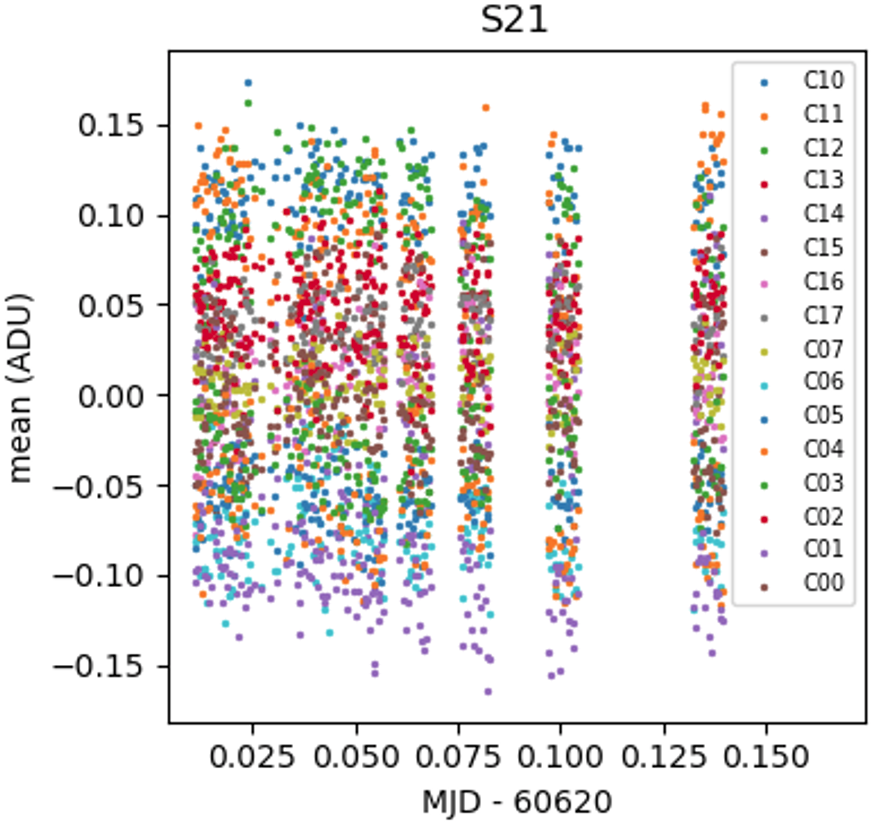
\includegraphics[width=0.9\textwidth]{sections/figures/E2136_R21_S21.png}
\end{centering}
\caption{Stable case (R21 S21)}
\end{figure}

\begin{figure}
\begin{centering}
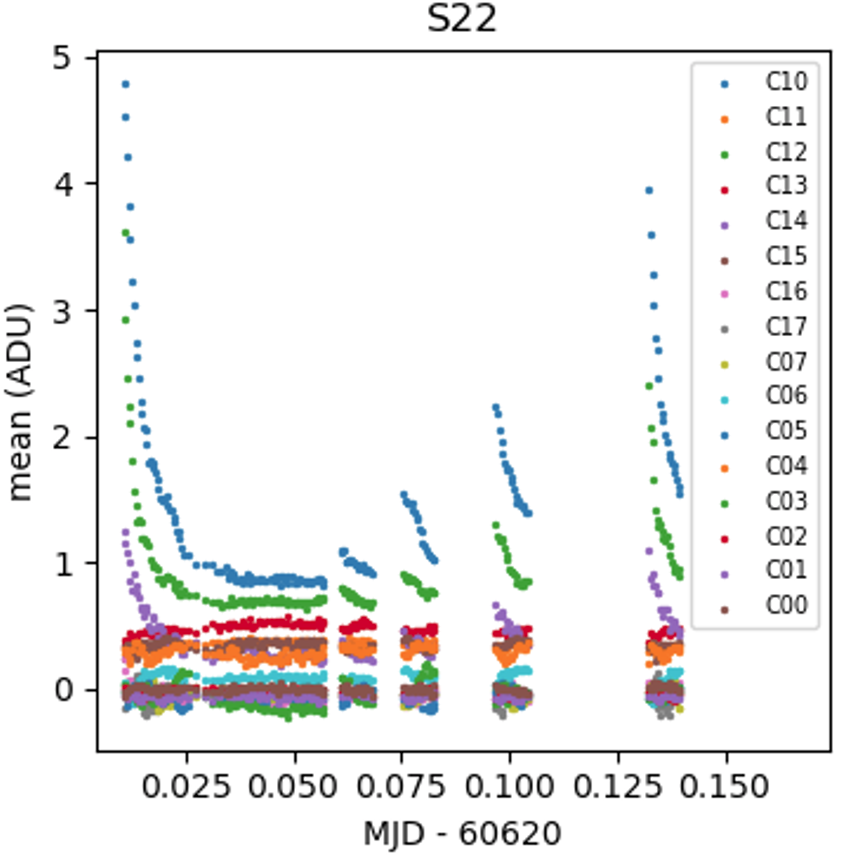
\includegraphics[width=0.9\textwidth]{sections/figures/E2136_R23_S22.png}
\end{centering}
\caption{Instable case (R23 S22)}
\end{figure}

A comparison of the results for an instable CDD is shown below for the
three runs.

\begin{figure}
\begin{centering}
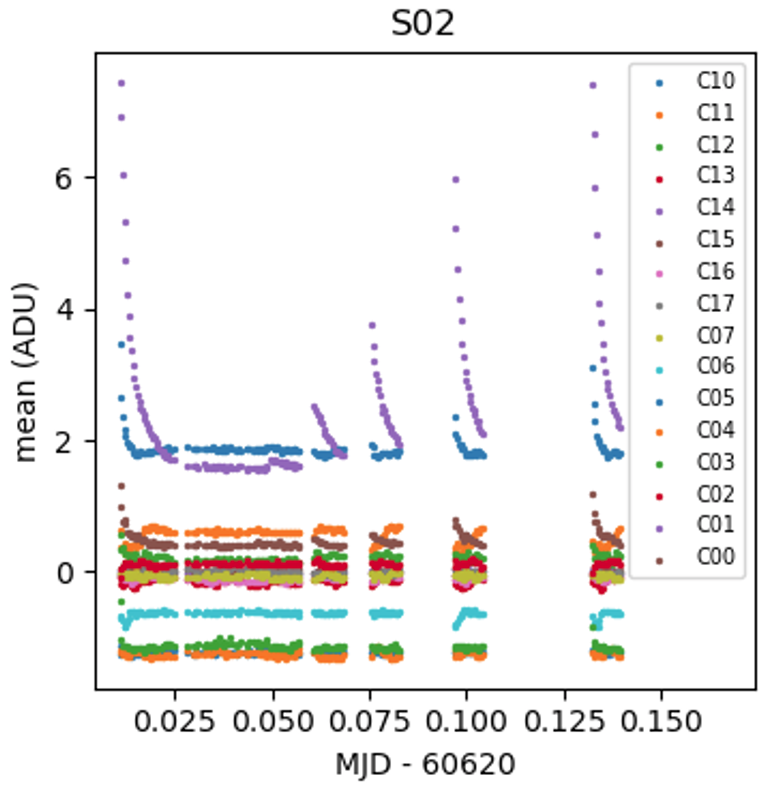
\includegraphics[width=0.9\textwidth]{sections/figures/E2136_R33_S02.png}
\end{centering}
\caption{Run E2136, R33 S02}
\end{figure}

\begin{figure}
\begin{centering}
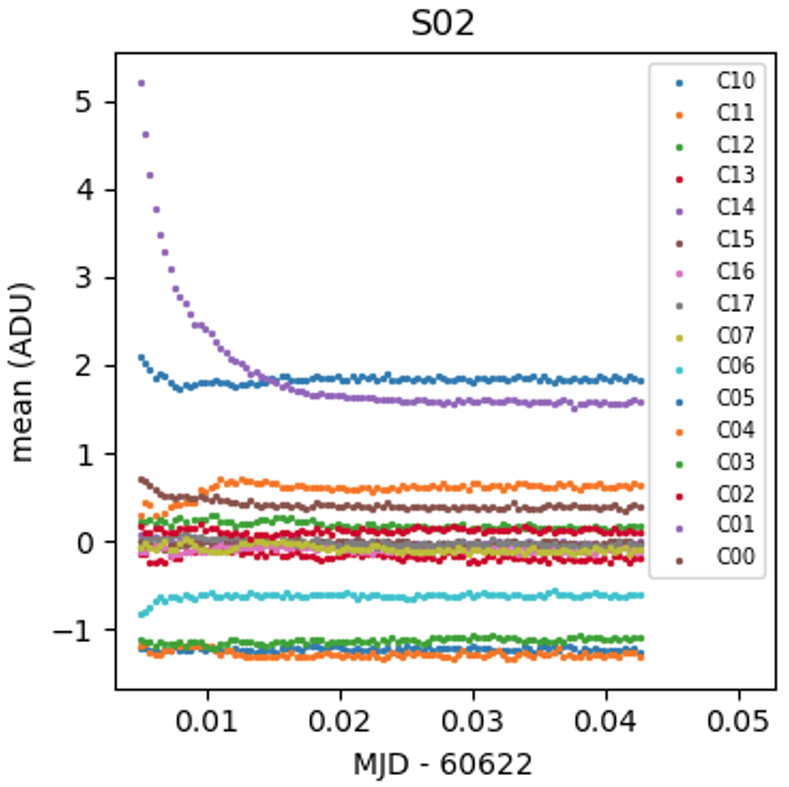
\includegraphics[width=0.9\textwidth]{sections/figures/E2236_R33_S02.png}
\end{centering}
\caption{Run E2236, R33 S02}
\end{figure}

\begin{figure}
\begin{centering}
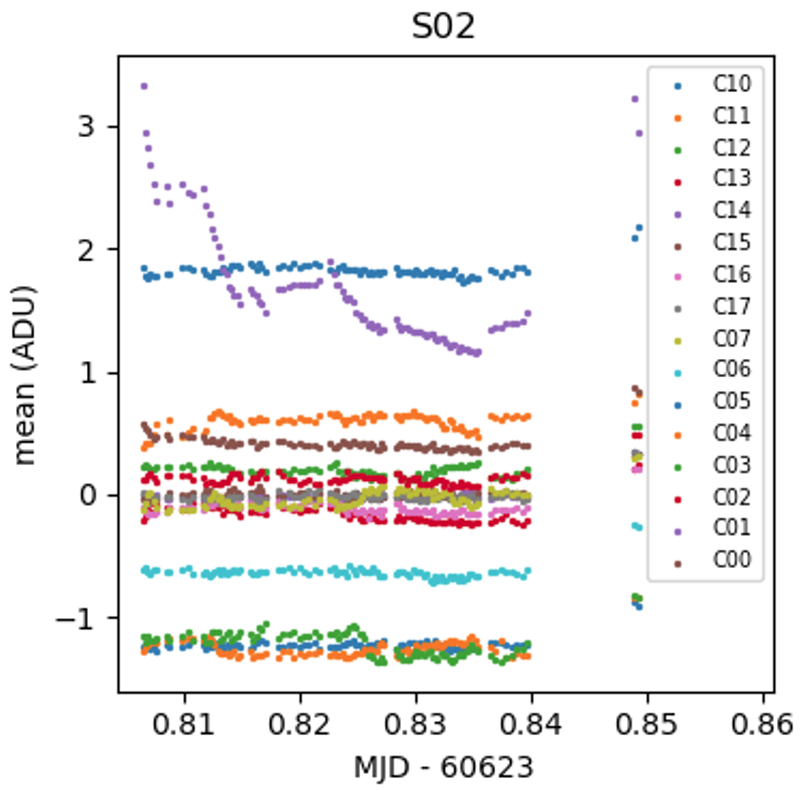
\includegraphics[width=0.9\textwidth]{sections/figures/E2330_R33_S02.png}
\end{centering}
\caption{Run E2330, R33 S02}
\end{figure}

In order to highlight the 2D shape differences, a 2D-overscan correction
is applied. A few exposures illustrating the variations of the 2D shape
for an instable CCD are shown below. The 2D shape of the image in
amplifier C01 is different in the 3 cases.

\begin{figure}
\begin{centering}
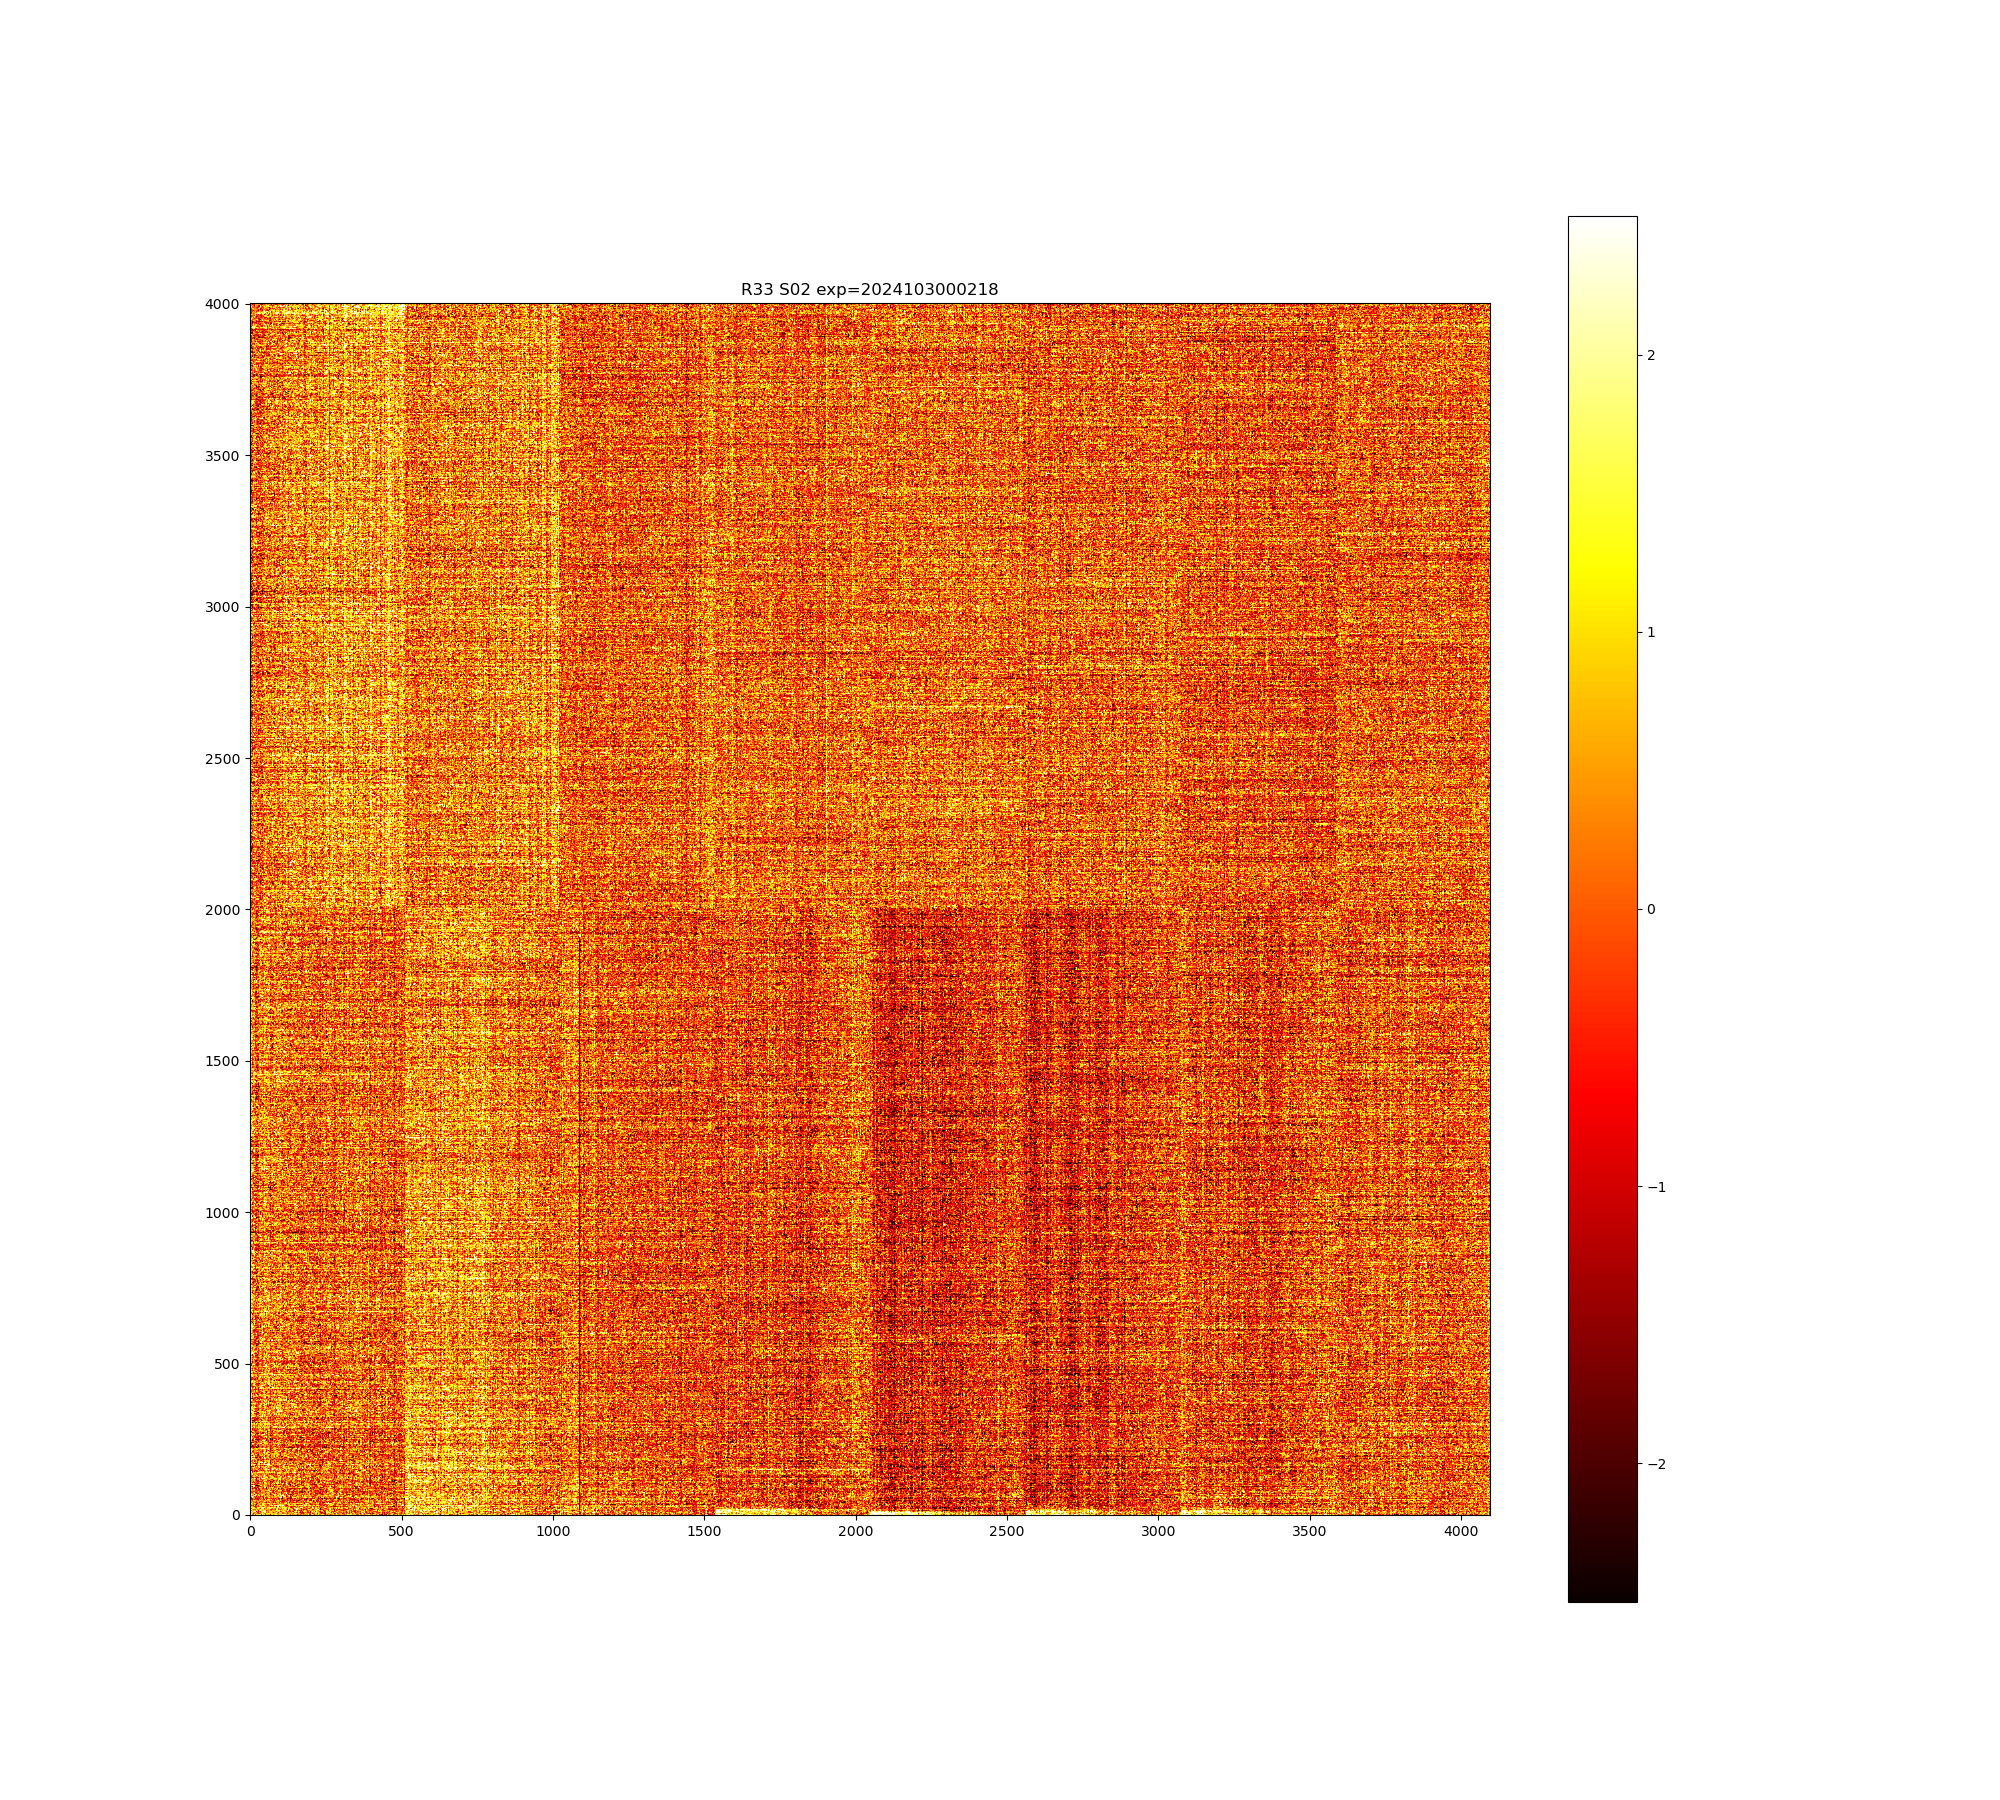
\includegraphics[width=0.9\textwidth]{sections/figures/E1880_bias_R33_S02.png}
\end{centering}
\caption{Bias exposure, run 1880, R33 S02}
\end{figure}

\begin{figure}
\begin{centering}
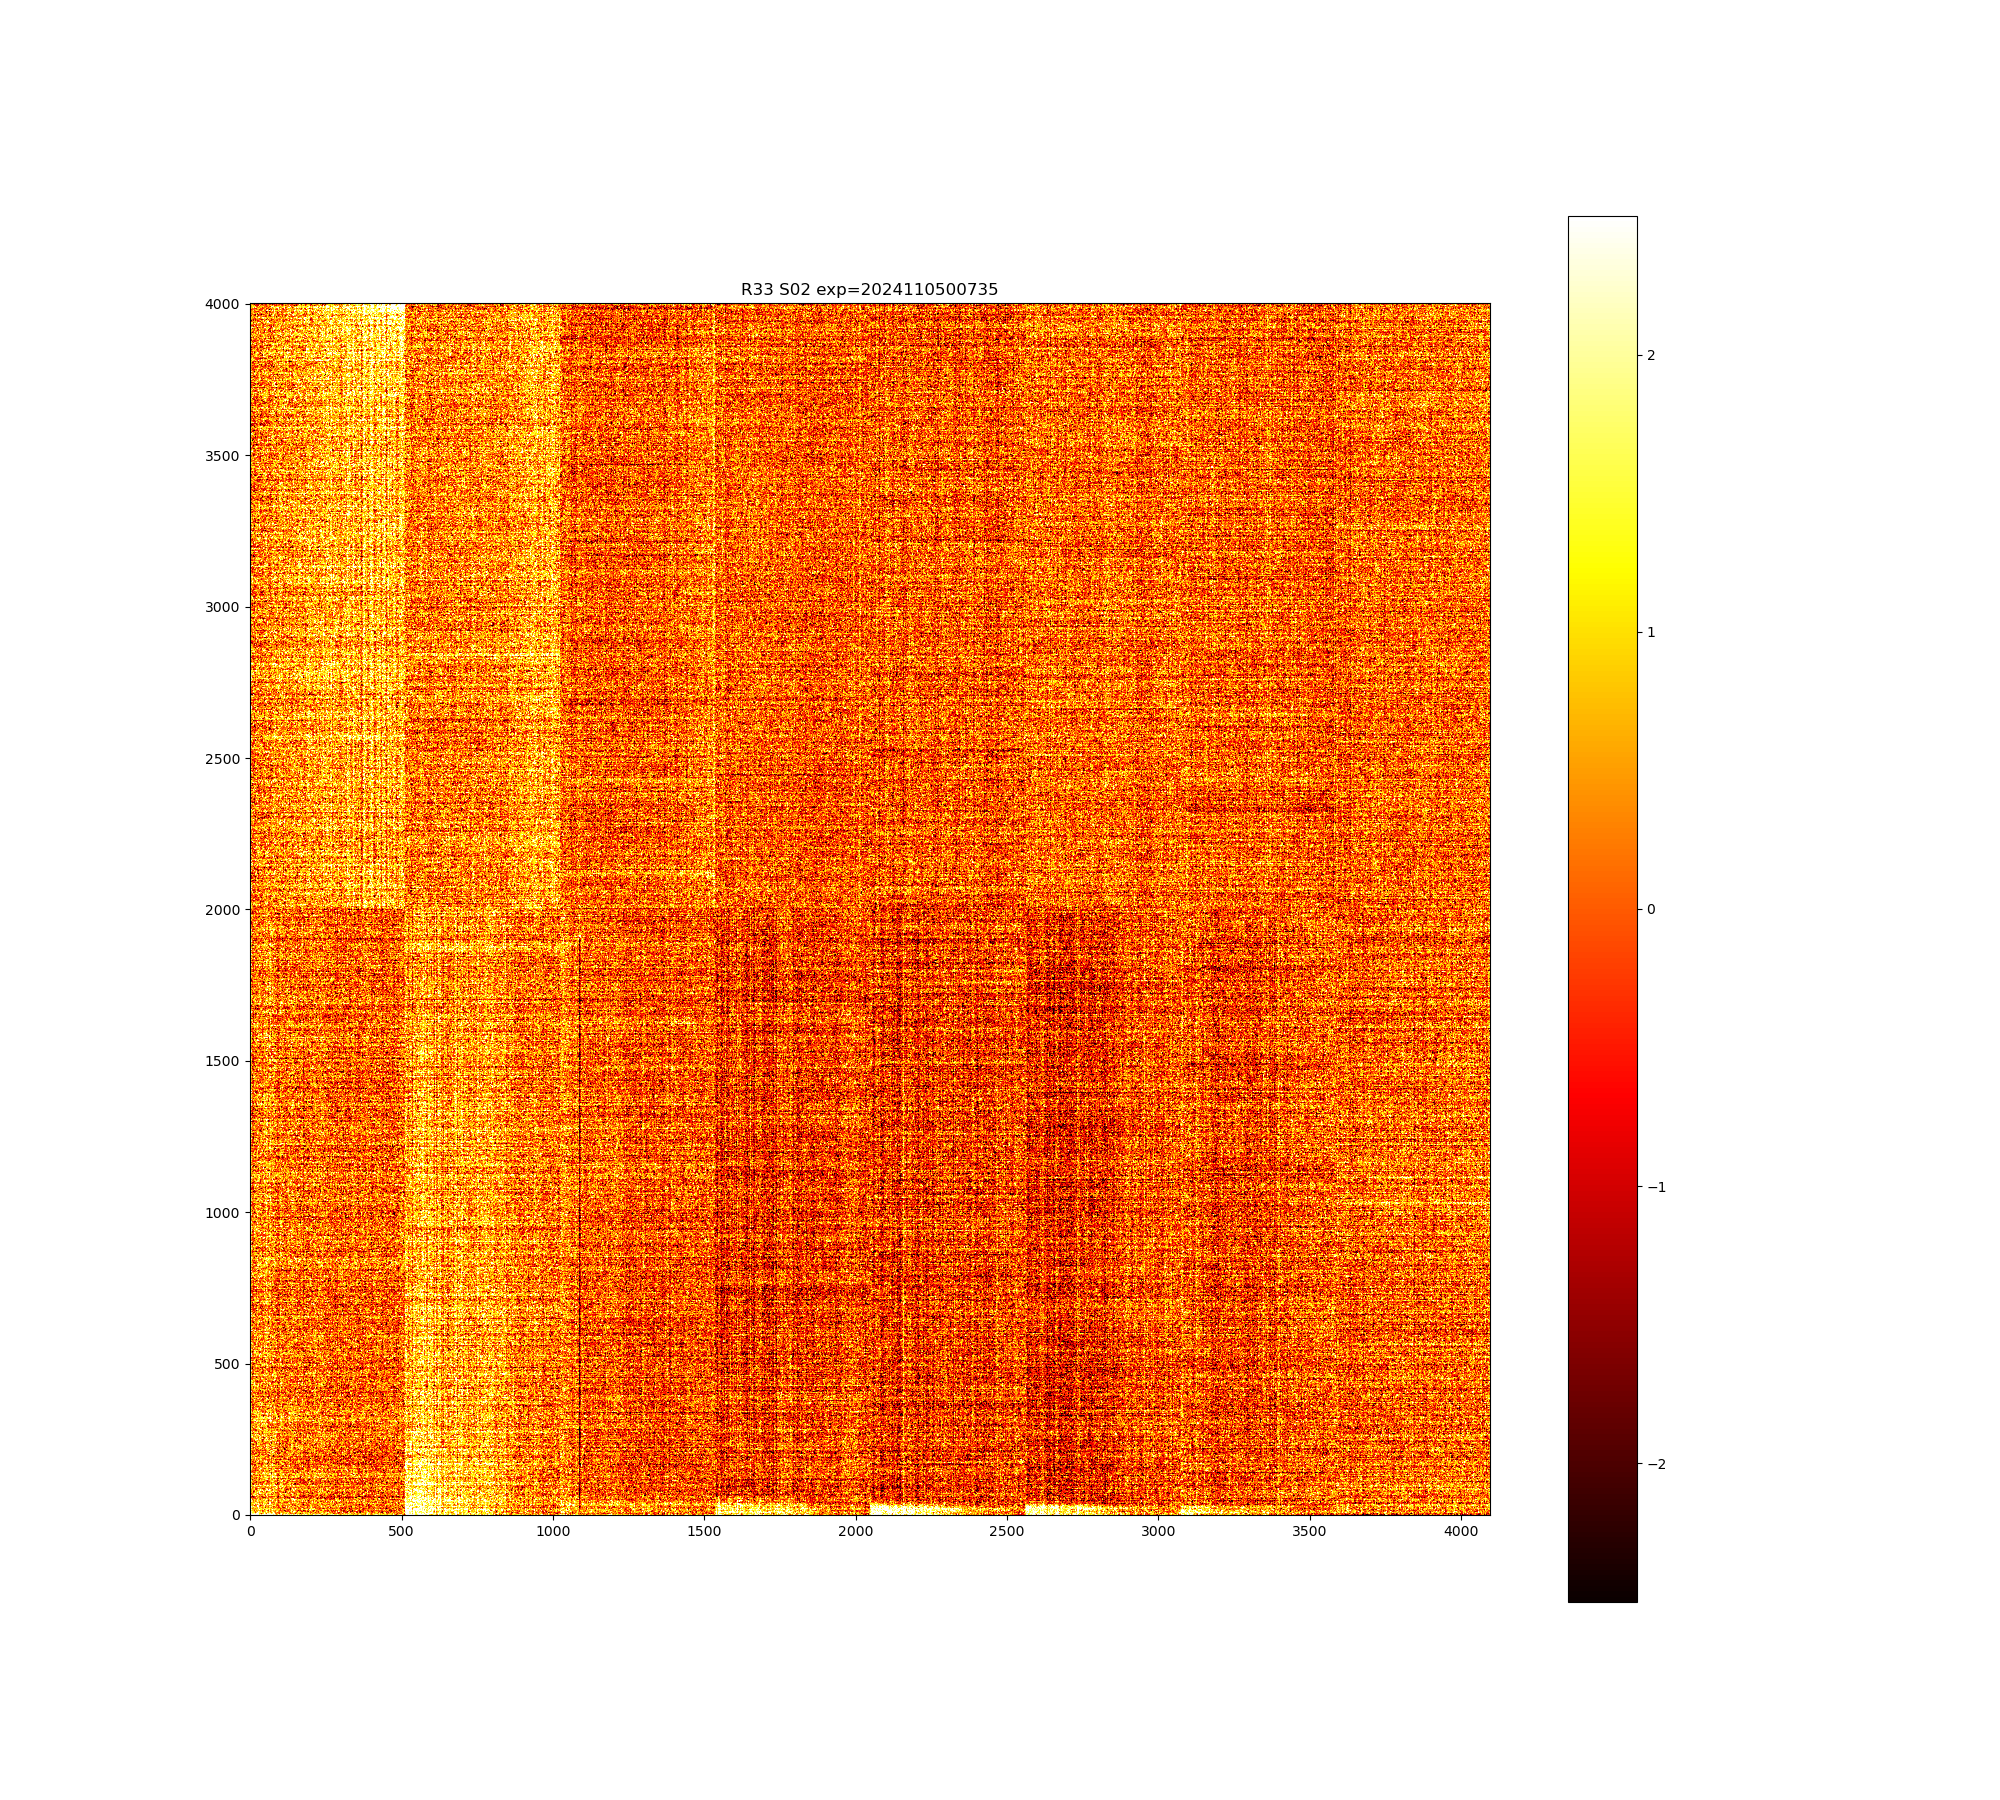
\includegraphics[width=0.9\textwidth]{sections/figures/E2136_dark15_R33_S02.png}
\end{centering}
\caption{15-s dark exposure, run E2136 in
\textquotesingle stable\textquotesingle{} conditions, R33 S02}
\end{figure}

\begin{figure}
\begin{centering}
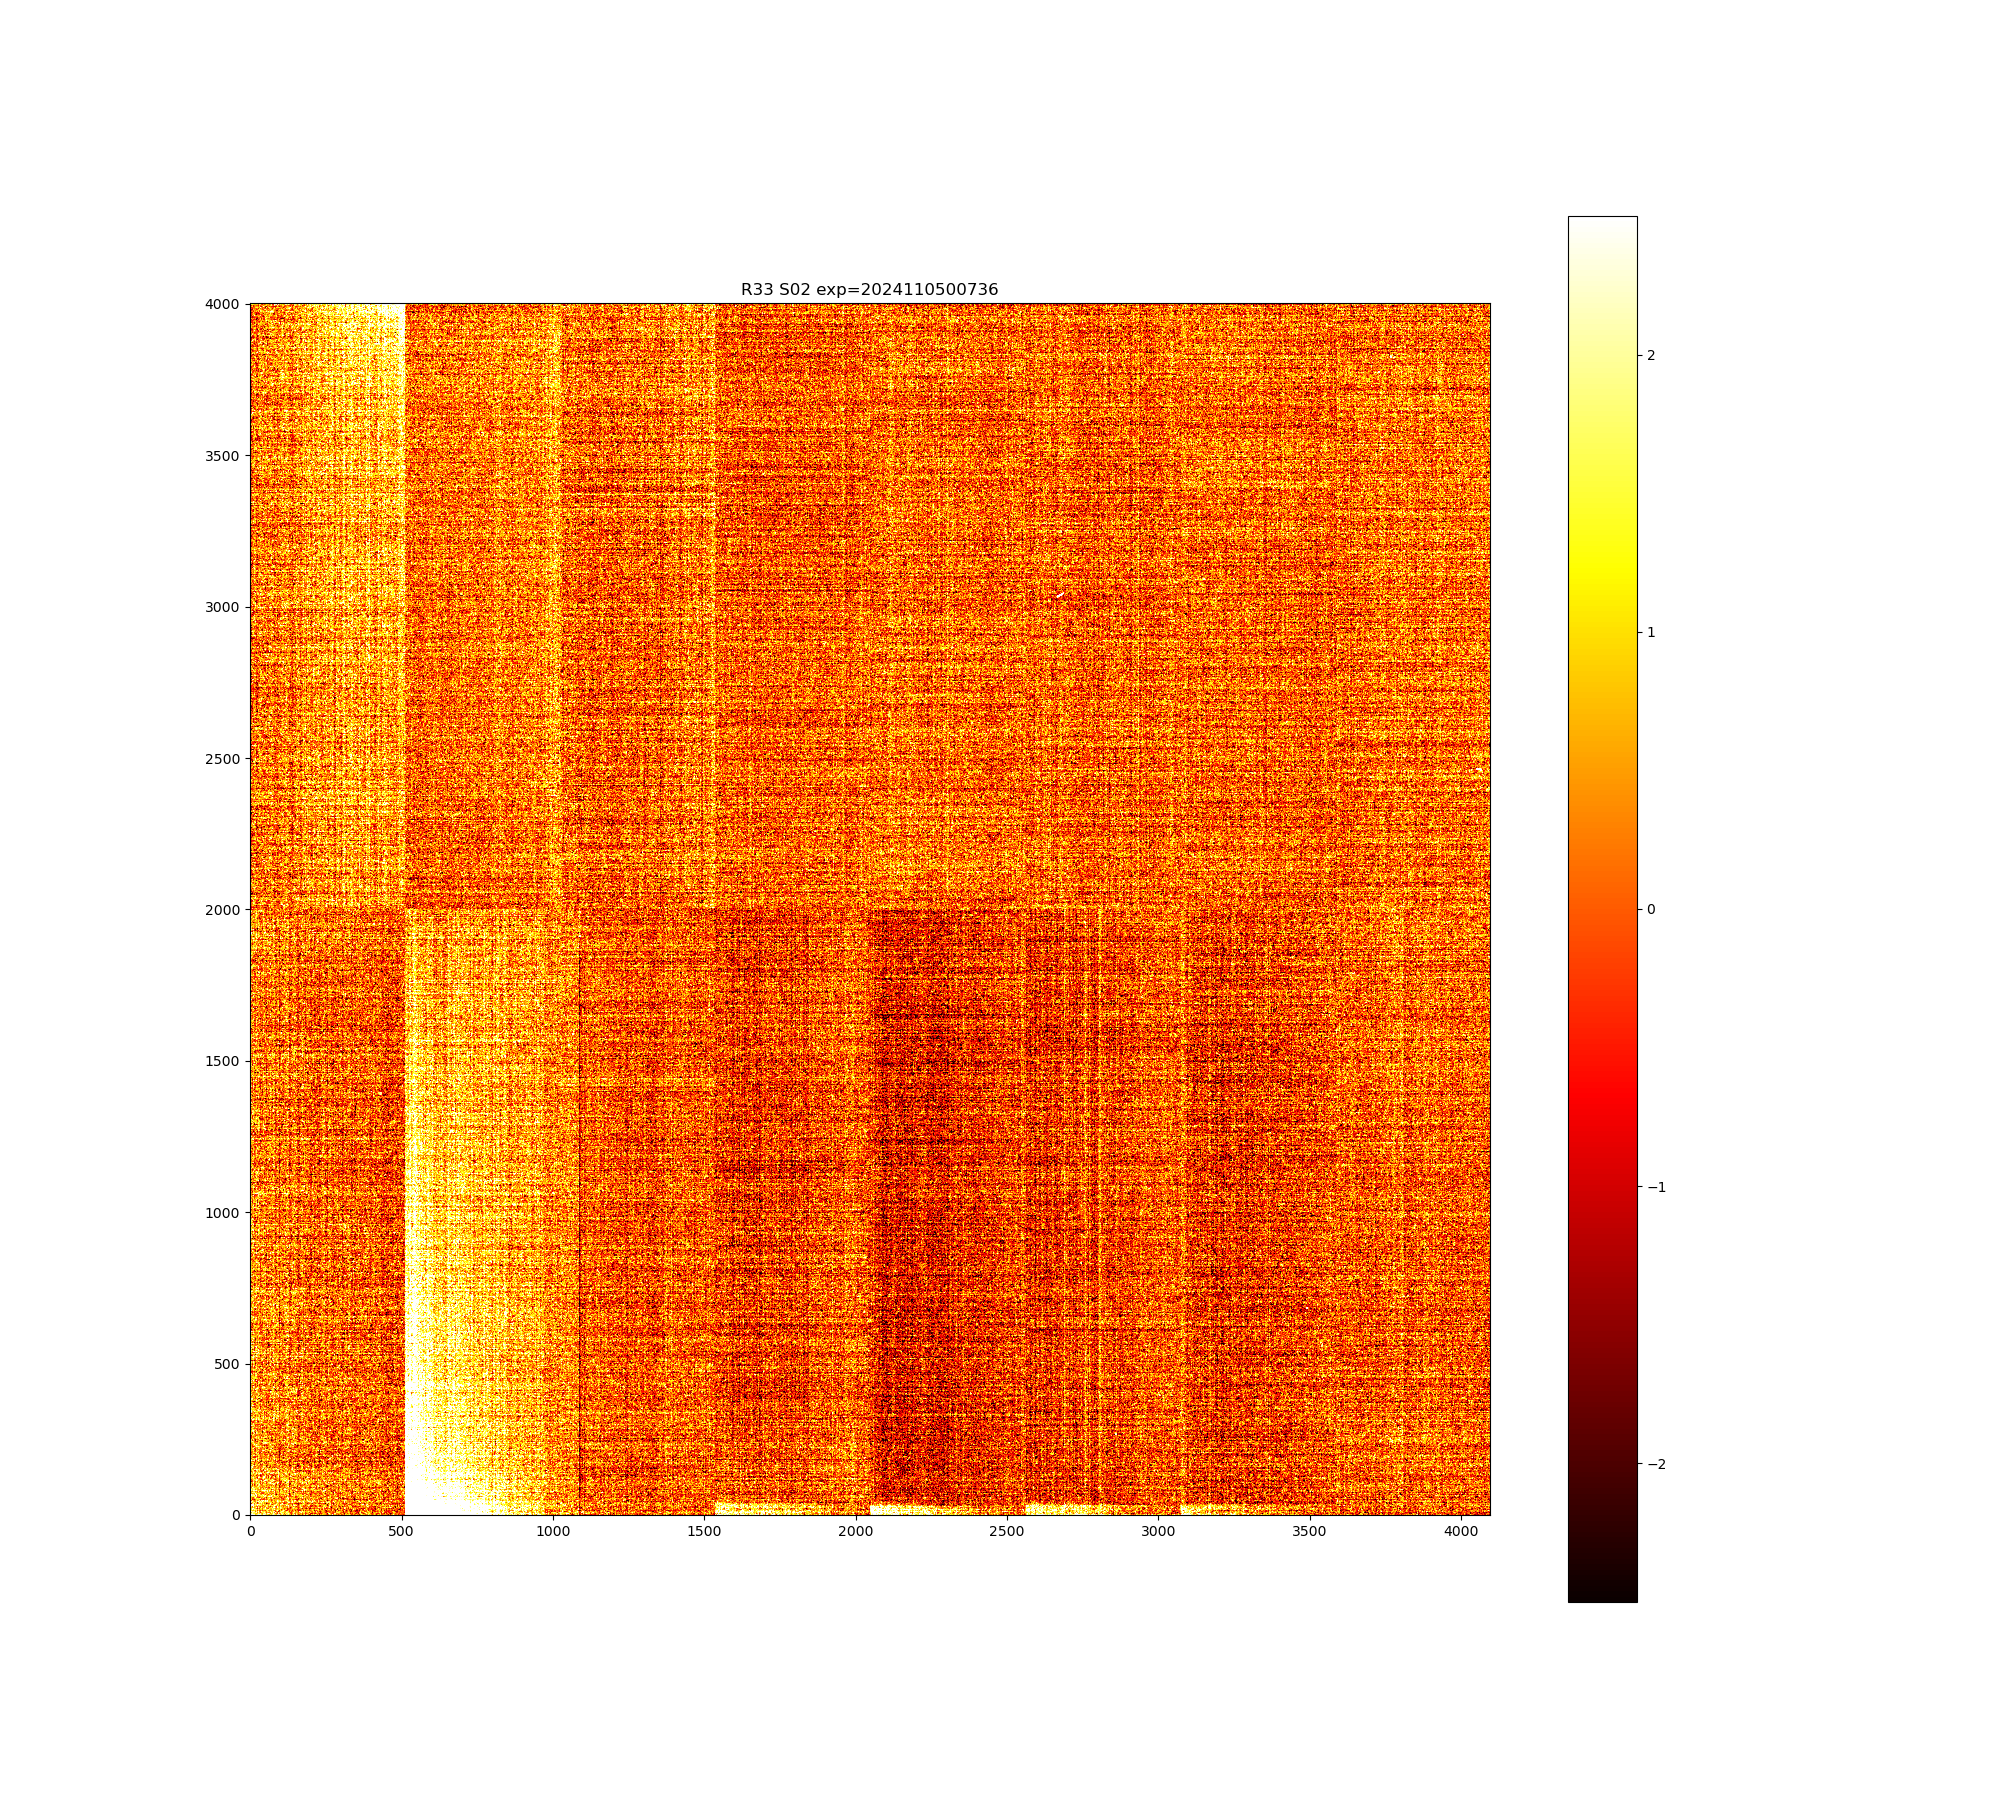
\includegraphics[width=0.9\textwidth]{sections/figures/E2136_dark15_delay_R33_S02.png}
\end{centering}
\caption{15-s dark exposure, run E2136 after a 3-minute delay, R33 S02}
\end{figure}

In order to quantify the number of e2v instable amplifiers, a stability
metric \emph{d} is defined from the eo\phantomsection\label{pipe}{pipe}
stability task data products. More precisely, \emph{d} is defined, for a
given amplifier in a given run, as the difference between the 5th and
95th percentiles of the image mean over all the exposures. The
distribution of \emph{d} for run E2136 is shown below. Applying a
threshold at 0.3, 51 amplifiers are identified as instable (see the
corresponding mosaic). This corresponds to \textasciitilde3\% of the e2v
amplifiers.

\begin{figure}
\begin{centering}
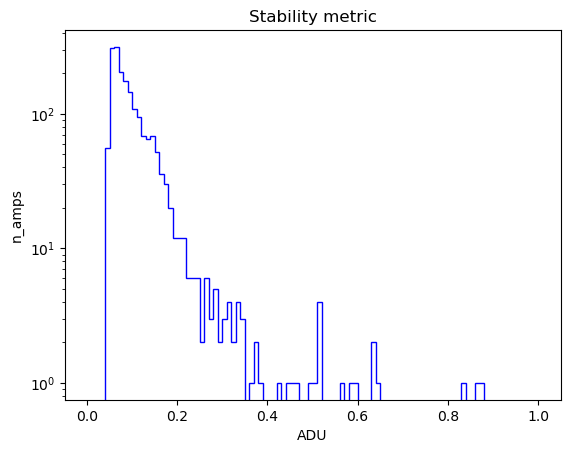
\includegraphics[width=0.9\textwidth]{sections/figures/E2136_distribution_d.png}
\end{centering}
\caption{Distribution of the stability metric for the e2v amplifiers in
run E2136}
\end{figure}

\begin{figure}
\begin{centering}
\includegraphics[width=0.9\textwidth]{sections/figures/E2136_mosaic_d.png}
\end{centering}
\caption{Mosaic of e2v amplifiers identified as instable (white color)
in run E2136}
\end{figure}

Further studies are required in order to converge on the best mitigation
strategy for the start of the LSST survey.

\subsection{Gain stability}\label{gain-stability-2}

hello world.

This section describes gain stability.

\begin{itemize}
\tightlist
\item
  No temp variation, fixed flux
\item
  no temp variation, variation in flux
\item
  Temp variation, fixed flux
\end{itemize}

\section{Sensor features}\label{sensor-features}

\subsection{Tree rings}\label{tree-rings}

\begin{figure}
\begin{centering}
\includegraphics[width=0.9\textwidth]{sections/figures/TR_centers.png}
\end{centering}
\caption{The center of the Tree Rings were measured for all 189 LSST sensors. Red point indicates the average center on each direction.}
\end{figure}

Radial study for Tree rings pattern has been done to see if the rings are perfectly circular in shape. 

This is the image of transforming the flat image into the radial image as the y axis to be the distance from the center of the rings. 

\begin{figure}
\begin{centering}
\includegraphics[width=0.9\textwidth]{sections/figures/TR_subtraction.png}
\end{centering}
\caption{Folding image on diagonal line from the center of the ring, and subtracting from each other.}
\end{figure}

\begin{figure}
\begin{centering}
\includegraphics[width=0.9\textwidth]{sections/figures/TR_radial.png}
\end{centering}
\caption{Radial study of the Tree Rings. Right: image subtracting left to right, right to left.}
\end{figure}

\begin{itemize}
\tightlist
\item
  Tree rings without diffuser
\item
  Tree rings with diffuser
\end{itemize}

\subsection{ITL Dips}\label{itl-dips}

One of the phenomenon that was stuided in the later part of Run 7 was
ITL dips. These were first discovered in LSST ComCam with on-sky data as
bleed trails from bright stars that traversed the entire detector,
jumping over the amplifier boundaries. These bleed trails are unique
though in that the core of the bleed trail is actually
\textquotesingle dark\textquotesingle{} compared to the wings of the
bleed trail, with a lower flux of around 2\% compared to the rest of the
bleed trail.

We tried to investigate if there were any ITL dips in the sensors of
LSSTCam. For this study, we used spots and rectangles created by a 4K
projector onto the focal plane. The spots were roughly 30 pixels across
and were in every amplifier of each detector. The rectangles were only
in the top right amplifier (C10). One unique feature with this spot
projection was that there was a background illumination caused by the
projector. This led to the spots having a signal only 6 times higher
than the background and the rectangles with a signal 30 times higher
than the background.

Investigating these images, we were not able to find any evidence of ITL
dips. Below are the images themselves along with binned horizontal
cutouts of the the amplifier below the source. These show the background
pattern of the projector, but no 2\% dip.

While we were not able to find evidence of the ITL dip in Run 7 data, it
is still not clear if this will not be visible in LSSTCam on-sky data.
The photon rate of the in-lab data was roughly XXX per second for the 15
second exposures. The stars that were seen in ComCam with the ITL dip
have a magnitude of XXX corresponding to a photon rate of XXX. This is
combined with a sky background of XXX as compared with the lab sensor
background of XXX.

\subsection{Vampire pixels}\label{vampire-pixels}

\subsubsection{First observations}\label{first-observations}

Vampire pixels were first observed in ComCam observations {[}need more
info to properly give context{]} - Andy\textquotesingle s study on Oct.
8 - Agnes masking effort

\subsubsection{LSSTCam vampire pixel
features}\label{lsstcam-vampire-pixel-features}

The vampire pixels have distinct features, both on the individual defect
level, and across the focal plane

\paragraph{Individual vampire
features}\label{individual-vampire-features}

\begin{itemize}
\tightlist
\item
  General size
\item
  Radial kernel
\item
  uniformity
\end{itemize}

\paragraph{Vampire features across the focal
plane}\label{vampire-features-across-the-focal-plane}

\begin{itemize}
\tightlist
\item
  sensor type
\item
  static or dynamic
\item
  higher concentrations? Particularly bad sensors?
\end{itemize}

\subsubsection{Current masking
conditions}\label{current-masking-conditions}

\begin{itemize}
\tightlist
\item
  Bright pixels
\item
  Dark pixels
\item
  Jim\textquotesingle s task
\end{itemize}

\subsubsection{Analysis of flats}\label{analysis-of-flats}

\begin{itemize}
\tightlist
\item
  LED effect
\item
  Intensity effect
\end{itemize}

\subsubsection{Analysis of darks}\label{analysis-of-darks}

\begin{itemize}
\tightlist
\item
  Previous LED effect
\item
  Intensity of LED effect
\item
  dark cadence and exposure times
\end{itemize}

\subsubsection{Current models of
vampires}\label{current-models-of-vampires}

\begin{itemize}
\tightlist
\item
  Tony \& Craig model
\item
  Others?
\end{itemize}



\subsection{Phosphorescence}\label{phosphorescence}

The Run7 persistence optimization process (cf. \S\ref{persistence-2}XX) used a short EO image acquisition sequence and analysis script, which rapidly provided persistence performance metrics as feedback for each configuration tested. Thus, as soon as the e2v sensors were shown to be nearly free of {\it their} undesirable effect by reducing their clock swing voltages from 9.3 down to 8.0 volts, a similar persistence (or memory effect) was immediately noticed, affecting a subset of the ITL sensors. This discovery gained immediate interest for at least two reasons: (1) that it had not been detected in prior EO campaigns, and (2) that the new memory effect on certain ITL sensors was morphologically distinct from what had just been cured on the e2vs. 

The ITL sensors with the largest memory effect were evaluated, and the following observations were made:
\begin{itemize}
    \item[1.] The morphology of the expressed memory effect in the first dark image acquired after the trigger (the saturation flat) was reminiscent of the {\it ``coffee stains''} seen on the same sensors in flat field response, but with the opposite polarity. The ``coffee stains'' are commonly assumed to be associated with minor, localized variations in the sensors' antireflective coatings or perhaps a very thin, dead layer associated with the backside surface: they tend to be larger in amplitude when shorter wavelengths are used to expose the sensors with flat field illumination.
    \item[2.] The timescale with which the memory effect attenuates, is curiously comparable to the timescales that were seen in the persistence suffered by the e2v sensors (which were allegedly due to exposure of surface states by the collected conversions, on the seniconductor-insulator interface on the front side): exponential time constants of between 20 and 40 seconds, which unfortunately are in turn very close to the nominal exposure cadence for Rubin's Survey.
    \item[3.] The similarity in memory effect time constants (de-trapping charges from surface states near the channel on the front side -- the e2v case -- vs. either de-trapping of charges located near the backside window surface or relaxation by photon emission by some excited states there -- the ITL case) can be thought to favor the electron de-trapping mechanism, just from the other surface. Otherwise, the nearly matched time constants would have to be seen as an improbable coincidence.
    \item[4.] A list of 12 ITL sensor serial numbers corresponding to those showing the memory effect was communicated to Mike Lesser at ITL. The list of parts shared certain properties according to his notes, and led him to develop a placeholder theory that would partially explain the mechanism. If true, it could explain what might be responsible for both the coffee stains and the memory effect with similar spatial distribution. He wrote that he tried, but was unsuccessful in diagnosing, using optical characterization tools (e.g. ellipsometer), any changes in optical constants on the affected regions of the ``stained'' sensors. The origin of the ``stains'', according to this theory, are primarily a byproduct of there being ``raised spots'' on the sensor's backside surface that survive the final silicon acid etch. The raised silicon areas could potentially be trapping ITL's resist during the cleaning process that directly follows the etching step. Lesser wrote that the resist is wax-based and {\it does} fluoresce. If the theory is correct, he suggests that the medium would definitely be located {\it under} the AR coating and related neither to the coating nor the oxidation processes.
    \item[5.] Discussions among the Rubin team led to the following distinction of terminology that served to name the ITL memory effect in question. We heard that main difference between ``fluorescence'' and ``phosphorescence'' in that the former is considered prompt re-emission and the later could re-emit following a finite characteristic time constant. Characteristic time constants are in the nanosecond scale for fluorescence, while for phosphorescence it would be in the milliseconds to seconds range. For the purpose of this discussion, we adopt the word ``phosphorescence'' to refer to the memory effect presence in ITL sensors.
    \item[6.] Mike Lesser mentioned that the wax-based resist fluoresces (that would be the prompt mechanism with very short relaxation time). If there is any such residual material between the coating and the passivated silicon, it would be natural to expect a halo that would accompany any sharp PSF image that passes through these ``stains'' on the sensor surface: a scatter term with low integrated amplitude, whose scale should depend upon the re-emission wavelength. This has not yet been seen in lab data but may appear once the Camera goes on-sky.
    
% I highly doubt that they are the resist itself but more likely etch patterns in the silicon itself which could have an effect on scattering and perhaps surface charge. But they could be initially caused by resist issues in during etching process.
% It’s rather obvious of course, but I checked the notes and device 231 was noted as “stained” during processing (after etching).
% In the past we did SEM work as well and could never get an answer on composition, thickness, etc.
\end{itemize}

\subsubsection{Measurement techniques for detecting and quantifying phosphorescence}\label{phos-measurement}
We mentioned above that certain phosphorescent morphologies strongly resemble the ``coffee stains'' seen on the same (ITL) sensors. It should be noted that measurement of the {\it shadow} caused by excess absorption (usually a couple percent) is a great deal simpler than collecting any deferred charge with adequate sensitivity and confidence. This section describes the methods used to identify the transient term we consider phosphorescence in the ITL sensors, and list the regions where it was detected. Following that, we describe in some detail the kinematics of its expression (cherry-picking specific easy-to-measure cases), together with the wavelength- and its excitation flux level dependence.

We parasitically used a series of {\it B-protocol} and {\it BOT-persistence} EO testing runs that were executed for the purpose of tuning the operation of e2v sensors. The reason for this was that the ITL operating parameters were left unchanged from run to run, and thereby gave us multiple instances of the same EO measurement conditions, although the acquisitions were captured over a span of a few weeks. The relevant EO runs acquired a series of dark images (with the nominal 15 second integration time, or `EXPTIME') that followed a deliberate overexposure and readout of a FLAT (CCOB LED `red', target signal 400000 electrons/pixel). The dark images acquired in succession following the FLAT image recorded the re-emitted or deferred signal collected within each 15 second period, and there were 20 such dark images acquired within each EO run. In all, we identified and analyzed a total of 22 runs containing this data, where the excitation flat had the properties described above. The first and the twentieth dark images were stacked and medianed following a nominal, instrumental signal removal (ISR) step. The twentieth median dark images were then subtracted from the first median darks. This further suppressed any remaining ISR residuals from the pixel data, which nominally now contain the {\it transient term} of the ITL phosphorescence, because as far as we could tell, the 15 second expression of the deferred signal 300 seconds after overexposure had almost completely attenuated.

Table~\ref{phosphorescence:datasets} provides the EO run IDs analyzed according to the process outlined above. Figures YY through ZZ display the transient term in 8x8 blocked images of the 12 rafts containing ITL sensors. These serve primarily to help identify which ITL sensors exhibit regions where we suspect presence of the phosphorescence effect. It should be noted that we retained the full 1x1 pixel resolution images for follow-up inspection, because there is no guarantee that the phosphorescence we see varies slowly with position.

\begin{longtable}[]{@{}
  >{\raggedright\arraybackslash}p{(\linewidth - 2\tabcolsep) * \real{0.2222}}
  >{\raggedright\arraybackslash}p{(\linewidth - 2\tabcolsep) * \real{0.3472}}@{}}
\caption{Zephyr Scale E-numbers and corresponding SeqIDs analyzed to estimate phosphorescence in ITL sensors}
\label{phosphorescence:datasets}\\
%\tabularnewline
\toprule\noalign{}
\begin{minipage}[b]{\linewidth}\raggedright
Detector type
\end{minipage} & \begin{minipage}[b]{\linewidth}\raggedright
\begin{quote}
File name
\end{quote}
\end{minipage} \\
\midrule\noalign{}
\endfirsthead
\toprule\noalign{}
\begin{minipage}[b]{\linewidth}\raggedright
Detector type
\end{minipage} & \begin{minipage}[b]{\linewidth}\raggedright
\begin{quote}
File name
\end{quote}
\end{minipage} \\
\midrule\noalign{}
\endhead
\bottomrule\noalign{}
\endlastfoot
\begin{minipage}[t]{\linewidth}\raggedright
\begin{quote}
E2V
\end{quote}
\end{minipage} &
FP\phantomsection\label{e2v_2s_l3cp_v30.seq}{E2V\_2s\_l3cp\_v30.seq} \\
\begin{minipage}[t]{\linewidth}\raggedright
\begin{quote}
ITL
\end{quote}
\end{minipage} &
FP\phantomsection\label{itl_2s_l3cp_v30.seq}{ITL\_2s\_l3cp\_v30.seq} \\
\end{longtable}


\begin{itemize}
\tightlist
\item
  phosphorescence background
\item
  phosphorescence on flat fields
\item
  phosphorescence on spot projections
\end{itemize}

\section{Conclusions}\label{conclusions}

\subsection{Run 7 final operating
parameters}\label{run-7-final-operating-parameters}

This section describes the conclusions of run 7 optimization and the
operating conditions of the camera. Decisions regarding these parameters
were decided based upon the results of the
\href{https://sitcomtn-148.lsst.io/\#persistence-optimization}{voltage
optimization},
\href{https://sitcomtn-148.lsst.io/\#sequencer-optimization}{sequencer
optimization}, and
\href{https://sitcomtn-148.lsst.io/\#thermal-optimization}{thermal
optimization}.

\subsubsection{Voltage conditions}\label{voltage-conditions}

\begin{longtable}[]{@{}
  >{\raggedright\arraybackslash}p{(\linewidth - 4\tabcolsep) * \real{0.1667}}
  >{\raggedright\arraybackslash}p{(\linewidth - 4\tabcolsep) * \real{0.2917}}
  >{\raggedright\arraybackslash}p{(\linewidth - 4\tabcolsep) * \real{0.2917}}@{}}
\caption{Voltage conditions}\tabularnewline
\toprule\noalign{}
\begin{minipage}[b]{\linewidth}\raggedright
Parameter
\end{minipage} & \begin{minipage}[b]{\linewidth}\raggedright
dp80 (new voltage)
\end{minipage} & \begin{minipage}[b]{\linewidth}\raggedright
dp93 (Run 5)
\end{minipage} \\
\midrule\noalign{}
\endfirsthead
\toprule\noalign{}
\begin{minipage}[b]{\linewidth}\raggedright
Parameter
\end{minipage} & \begin{minipage}[b]{\linewidth}\raggedright
dp80 (new voltage)
\end{minipage} & \begin{minipage}[b]{\linewidth}\raggedright
dp93 (Run 5)
\end{minipage} \\
\midrule\noalign{}
\endhead
\bottomrule\noalign{}
\endlastfoot
pclkHigh & \begin{minipage}[t]{\linewidth}\raggedright
\begin{quote}
2.0
\end{quote}
\end{minipage} & \begin{minipage}[t]{\linewidth}\raggedright
\begin{quote}
3.3
\end{quote}
\end{minipage} \\
pclkLow & \begin{minipage}[t]{\linewidth}\raggedright
\begin{quote}
-6.0
\end{quote}
\end{minipage} & \begin{minipage}[t]{\linewidth}\raggedright
\begin{quote}
-6.0
\end{quote}
\end{minipage} \\
dpclk & \begin{minipage}[t]{\linewidth}\raggedright
\begin{quote}
8.0
\end{quote}
\end{minipage} & \begin{minipage}[t]{\linewidth}\raggedright
\begin{quote}
9.3
\end{quote}
\end{minipage} \\
sclkHigh & \begin{minipage}[t]{\linewidth}\raggedright
\begin{quote}
3.55
\end{quote}
\end{minipage} & \begin{minipage}[t]{\linewidth}\raggedright
\begin{quote}
3.9
\end{quote}
\end{minipage} \\
sclkLow & \begin{minipage}[t]{\linewidth}\raggedright
\begin{quote}
-5.75
\end{quote}
\end{minipage} & \begin{minipage}[t]{\linewidth}\raggedright
\begin{quote}
-5.4
\end{quote}
\end{minipage} \\
rgHigh & \begin{minipage}[t]{\linewidth}\raggedright
\begin{quote}
5.01
\end{quote}
\end{minipage} & \begin{minipage}[t]{\linewidth}\raggedright
\begin{quote}
6.1
\end{quote}
\end{minipage} \\
rgLow & \begin{minipage}[t]{\linewidth}\raggedright
\begin{quote}
-4.99
\end{quote}
\end{minipage} & \begin{minipage}[t]{\linewidth}\raggedright
\begin{quote}
-4.0
\end{quote}
\end{minipage} \\
rd & \begin{minipage}[t]{\linewidth}\raggedright
\begin{quote}
10.5
\end{quote}
\end{minipage} & \begin{minipage}[t]{\linewidth}\raggedright
\begin{quote}
11.6
\end{quote}
\end{minipage} \\
od & \begin{minipage}[t]{\linewidth}\raggedright
\begin{quote}
22.3
\end{quote}
\end{minipage} & \begin{minipage}[t]{\linewidth}\raggedright
\begin{quote}
23.4
\end{quote}
\end{minipage} \\
og & \begin{minipage}[t]{\linewidth}\raggedright
\begin{quote}
-3.75
\end{quote}
\end{minipage} & \begin{minipage}[t]{\linewidth}\raggedright
\begin{quote}
-3.4
\end{quote}
\end{minipage} \\
gd & \begin{minipage}[t]{\linewidth}\raggedright
\begin{quote}
26.0
\end{quote}
\end{minipage} & \begin{minipage}[t]{\linewidth}\raggedright
\begin{quote}
26.0
\end{quote}
\end{minipage} \\
\end{longtable}

\subsubsection{Sequencer conditions}\label{sequencer-conditions}

\begin{longtable}[]{@{}
  >{\raggedright\arraybackslash}p{(\linewidth - 2\tabcolsep) * \real{0.2222}}
  >{\raggedright\arraybackslash}p{(\linewidth - 2\tabcolsep) * \real{0.3472}}@{}}
\caption{Sequencer conditions}\tabularnewline
\toprule\noalign{}
\begin{minipage}[b]{\linewidth}\raggedright
Detector type
\end{minipage} & \begin{minipage}[b]{\linewidth}\raggedright
\begin{quote}
File name
\end{quote}
\end{minipage} \\
\midrule\noalign{}
\endfirsthead
\toprule\noalign{}
\begin{minipage}[b]{\linewidth}\raggedright
Detector type
\end{minipage} & \begin{minipage}[b]{\linewidth}\raggedright
\begin{quote}
File name
\end{quote}
\end{minipage} \\
\midrule\noalign{}
\endhead
\bottomrule\noalign{}
\endlastfoot
\begin{minipage}[t]{\linewidth}\raggedright
\begin{quote}
E2V
\end{quote}
\end{minipage} &
FP\phantomsection\label{e2v_2s_l3cp_v30.seq}{E2V\_2s\_l3cp\_v30.seq} \\
\begin{minipage}[t]{\linewidth}\raggedright
\begin{quote}
ITL
\end{quote}
\end{minipage} &
FP\phantomsection\label{itl_2s_l3cp_v30.seq}{ITL\_2s\_l3cp\_v30.seq} \\
\end{longtable}

\begin{itemize}
\tightlist
\item
  v30 sequencers are identical to the
  FP\phantomsection\label{itl_2s_l3cp_v29_noppp.seq}{ITL\_2s\_l3cp\_v29\_Noppp.seq}
  and
  FP\phantomsection\label{e2v_2s_l3cp_v29_nopsf.seq}{E2V\_2s\_l3cp\_v29\_NopSf.seq}.
  All sequencer files can be found in the
  \href{https://github.com/lsst-camera-dh/sequencer-files/tree/master/run7}{github
  repository}.
\end{itemize}

\subsubsection{Other camera conditions}\label{other-camera-conditions}

\begin{itemize}
\tightlist
\item
  Idle flush disabled
\end{itemize}

\subsection{Record runs}\label{record-runs}

This section describes run 7 record runs.

All runs use our camera operating configuration, unless otherwise noted.

\begin{longtable}[]{@{}
  >{\raggedright\arraybackslash}p{(\linewidth - 6\tabcolsep) * \real{0.1421}}
  >{\raggedright\arraybackslash}p{(\linewidth - 6\tabcolsep) * \real{0.0474}}
  >{\raggedright\arraybackslash}p{(\linewidth - 6\tabcolsep) * \real{0.0421}}
  >{\raggedright\arraybackslash}p{(\linewidth - 6\tabcolsep) * \real{0.7579}}@{}}
\caption{Record runs}\tabularnewline
\toprule\noalign{}
\begin{minipage}[b]{\linewidth}\raggedright
Run Type
\end{minipage} & \begin{minipage}[b]{\linewidth}\raggedright
Run ID
\end{minipage} & \begin{minipage}[b]{\linewidth}\raggedright
Links
\end{minipage} & \begin{minipage}[b]{\linewidth}\raggedright
Notes
\end{minipage} \\
\midrule\noalign{}
\endfirsthead
\toprule\noalign{}
\begin{minipage}[b]{\linewidth}\raggedright
Run Type
\end{minipage} & \begin{minipage}[b]{\linewidth}\raggedright
Run ID
\end{minipage} & \begin{minipage}[b]{\linewidth}\raggedright
Links
\end{minipage} & \begin{minipage}[b]{\linewidth}\raggedright
Notes
\end{minipage} \\
\midrule\noalign{}
\endhead
\bottomrule\noalign{}
\endlastfoot
\multirow{2}{=}{B protocol} & E1880 & & \\
& E2233 & & Identical to E1880. Acquired after CCS subsystem reboot \\
\multirow{5}{=}{PTCs} & E1886 & & Red LED dense. Dark interleaving
between flat pairs \\
& E1881 & & Red LED dense. No dark interleaving between flat pairs \\
& E748 & & nm960 dense \\
& E2237 & & Red LED dense. Acquired after CCS subsystem reboot. \\
& E2016 & & Super dense red LED. HV Bias off for R13/Reb2. jGroups
meltdown interrupted acquisitions, restarted \\
\multirow{5}{=}{Long dark acquisitions} & E1117 & & \\
& E1116 & & \\
& E1115 & & \\
& E1114 & & \\
& E1075 & & \\
\multirow{5}{=}{Projector acquisitions} & E1558 & & Flat pairs, fine
scan in flux from 1-100s in 1s intervals.
E2V:v29\phantomsection\label{nop}{NoP},
ITL:v29\phantomsection\label{nopp}{NoPP} \\
& E1553 & & Flat pairs, coarse scan in flux from 5-120s in 5s
interval.E2V:v29\phantomsection\label{nop}{NoP},
ITL:v29\phantomsection\label{nopp}{NoPP} \\
& E1586 & & One 100s flat exposure, spots moved to selected
phosphorescent regions.E2V:v29\phantomsection\label{nop}{NoP},
ITL:v29\phantomsection\label{nopp}{NoPP} \\
& E2181 & & Flat pairs from 2-60s in 2s intervals. Two 15s darks
interleaved after flat acquisition. Rectangle on C10
amplifier.E2V:v29\phantomsection\label{nop}{NoP},
ITL:v29\phantomsection\label{nopp}{NoPP} \\
& E2184 & & 10 30s dark images to capture background pattern \\
\multirow{5}{=}{OpSim runs} & E1717 & & Long dark sequence, no filter
changes \\
& E2330 & & Short dark sequence, filter changes in headers through
OCS \\
& E1414 & & 30 minutes OpSim run with shutter control, filter change,
and realistic survey cadence \\
& E2328 & & Flats with shutter-controlled exposure \\
& E1657 & & 10 hour OpSim dark run, \textasciitilde50\% of darks were
acquired properly \\
\multirow{5}{=}{Phosphorescence datasets} & E2015 & & 10 flats at 10ke-
followed by 10x15s darks \\
& E2014 & & 1 flat at 10ke- followed by 10x15s darks \\
& E2011 & & 20 flats at 10ke- followed by 10x15s darks \\
& E2012 & & 10 flats at 1ke- followed by 10x15 s darks \\
& E2013 & & 10 flats at 10ke- followed by 10x15s darks. Interleaved
biases with the darks \\
\multirow{10}{=}{Tree ring flats} & E1050 & & \\
& E1052 & & \\
& E1053 & & \\
& E1055 & & \\
& E1056 & & \\
& E1021 & & \\
& E1023 & & \\
& E1024 & & \\
& E1025 & & \\
& E1026 & & \\
\multirow{7}{=}{Gain stability runs} & E1955 & & \\
& E2008 & & \\
& E1968 & & \\
& E1367 & & \\
& E1362 & & \\
& E756 & & \\
& E1496 & & \\
\multirow{25}{=}{Persistence datasets} & E1503 & & \\
& E1504 & & \\
& E1505 & & \\
& E1506 & & \\
& E2286 & & \\
& E1502 & & \\
& E1501 & & \\
& E1500 & & \\
& E1499 & & \\
& E1498 & & \\
& E1494 & & \\
& E1493 & & \\
& E1492 & & \\
& E1490 & & \\
& E1491 & & \\
& E1489 & & \\
& E1488 & & \\
& E1487 & & \\
& E1486 & & \\
& E1485 & & \\
& E1478 & & \\
& E1477 & & \\
& E1479 & & \\
& E1483 & & \\
& E1484 & & \\
\multirow{12}{=}{Guider ROI acquisitions} & E1510 & & \\
& E1518 & & \\
& E1519 & & \\
& E1508 & & \\
& E1509 & & \\
& E1520 & & \\
& E1511 & & \\
& E1521 & & \\
& E1512 & & \\
& E1513 & & \\
& E1514 & & \\
& E1517 & & \\
\end{longtable}

\phantomsection\label{citations}
\begin{description}
\item[\label{A2023}{A2023}]
\url{https://arxiv.org/pdf/2301.03274}
\item[\label{Astier}{Astier}]
\url{https://www.aanda.org/articles/aa/abs/2019/09/aa35508-19/aa35508-19.html}
\item[\label{Bipolar}{Bipolar}]
\url{https://github.com/lsst-camera-dh/mkconfigs/blob/master/newformula.py}
\item[\label{D2014}{D2014}]
\url{https://ui.adsabs.harvard.edu/abs/2014SPIE.9154E}..18D/abstract
\item[\label{DavisReport}{DavisReport}]
\url{https://docs.google.com/document/d/1V4o9tzKBLnI1nlOlMFImPko8pDkD6qE7jzzk-duE-Qo/edit?tab=t.0\#heading=h.frkqtvvyydkr}
\item[\label{EPER}{EPER}]
\url{https://www.spiedigitallibrary.org/journals/Journal-of-Astronomical-Telescopes-Instruments-and-Systems/volume-7/issue-4/048002/Characterization-and-correction-of-serial-deferred-charge-in-LSST-camera/10.1117/1.JATIS.7.4.048002.full}
\item[\label{J2001}{J2001}]
\url{https://www.spiedigitallibrary.org/ebooks/PM/Scientific-Charge-Coupled-Devices/eISBN-9780819480392/10.1117/3.374903}
\item[\label{Persistence}{Persistence}]
\url{https://dmtn-276.lsst.io/}
\item[\label{PersistenceMitigationVoltage}{PersistenceMitigationVoltage}]
\url{https://github.com/lsst-camera-dh/e2v_voltages/blob/main/setup_e2v_v4.py}
\item[\label{S2024}{S2024}]
\url{https://ui.adsabs.harvard.edu/abs/2024SPIE13103E}..21S/abstract
\item[\label{U2024}{U2024}]
\url{https://ui.adsabs.harvard.edu/abs/2024SPIE13103E}..0WU/abstract
\item[\label{dmtn-276}{dmtn-276}]
\url{https://dmtn-276.lsst.io}
\item[\label{sequencerV23_DC}{sequencerV23\_DC}]
\url{https:parallelgithub.com/lsst-camera-dh/sequencer-files/blob/master/run5/FP_E2V_2s_ir2_v23_DC.seq}
\item[\label{sequencerV29}{sequencerV29}]
\url{https:parallelgithub.com/lsst-camera-dh/sequencer-files/blob/master/Run}
7/FP\phantomsection\label{e2v_2s_l3cp_v29.seq}{E2V\_2s\_l3cp\_v29.seq}
\item[\label{sequencerV29_NoP}{sequencerV29\_NoP}]
\url{https:parallelgithub.com/lsst-camera-dh/sequencer-files/blob/master/Run}
7/FP\phantomsection\label{e2v_2s_l3cp_v29_nop.seq}{E2V\_2s\_l3cp\_v29\_Nop.seq}
\item[\label{sequencerV29_NoPSF}{sequencerV29\_NoPSF}]
\url{https:parallelgithub.com/lsst-camera-dh/sequencer-files/blob/master/Run}
7/FP\phantomsection\label{e2v_2s_l3cp_v29_nopsf.seq}{E2V\_2s\_l3cp\_v29\_NopSf.seq}
\end{description}

\appendix
\section{FCS work}

\section{CCS work}
\subsection{JGroups issue}

\section{OCS integration}